%& -shell-escape -enable-write18 
% la riga sopra non funziona!
\typeout{*******************************************************************************}
\typeout{RENDERING RIASSUNTI DI FISICA INIZIATO}
\typeout{*******************************************************************************}
\typeout{Qualcuno, non sapendo verso quali disgrazie va incontro, si accinge a renderizzare: buona fortuna!}
\typeout{}\typeout{}\typeout{}

%********************************DICHIARAZIONE DOCUMENTO***********************
%***********PACCHETTI GRAFICI E THUMBDF E HYPEREF******************************

\documentclass[a4paper,12pt,twoside,openany,italian]{book}
\usepackage{ifpdf}

\ifpdf
\typeout{RENDERING PDF - PDF - PDF - PDF}
\usepackage[pdftex]{graphicx}
\DeclareGraphicsExtensions{.pdf,.png,.jpg, .jpeg, .mps,.gif}
\RequirePackage[pdftex,hyperindex,colorlinks]{hyperref}
%\usepackage{thumbpdf}
\pdfcompresslevel=9
\hypersetup{
	pdftitle={Un mini-corso sulla Relatività di Einstein},
	pdfauthor={CristianCantoro},
	pdfkeywords={relatività,ristretta,generale, Einstein},
	pdfpagemode=UseThumbs,
	pdfpagelayout=OneColumn
}
\else
\typeout{RENDERING DVI - NON PDF - NON PDF - NON PDF}
\usepackage[dvips]{graphicx}
\RequirePackage[dvipdfm,hyperindex,colorlinks]{hyperref}
\fi
\typeout{}\typeout{}

\pdfoptionpdfminorversion=6

%********************************PACCHETTI*************************************
\usepackage[utf8]{inputenc}
\usepackage[italian]{babel}
%\usepackage[T1]{fontenc}
\usepackage{ulem} %testo strikkato
\usepackage[grey,palatino]{quotchap}
\usepackage{bm}
\usepackage{amsfonts,amstext,amsmath,amssymb}
\usepackage[alsoload=hep]{siunitx}
\usepackage{makeidx}
\usepackage{subfigure}
\usepackage{wrapfig}
\usepackage{theorem}
\usepackage{fancyhdr}
\usepackage{syntonly}
\usepackage[all]{xy}
\usepackage{xmpincl}
\usepackage{svn}
\usepackage[version=3]{mhchem}
%\usepackage{ctable}
\usepackage{empheq}
%\usepackage{xcolor}
\usepackage{tikz}
\usepackage[tight,italian]{minitoc}
%*******************************VERSIONE***************************************

\newcommand{\versione}{0.4}

%******************************SYNTAX******************************************
% decommentare la riga sotto, se si vuole solo controllare la sintassi del
% documento, senza produrre un output, è molto più veloce
%
%\syntaxonly

%********************************DEFINIZIONI MATEMATICHE***********************
\DeclareMathOperator{\grad}{grad}
\DeclareMathOperator{\diver}{div}
\DeclareMathOperator{\rot}{rot}
\DeclareMathOperator{\arcsinh}{arcsinh}
\DeclareMathOperator{\arccosh}{arccosh}
\DeclareMathOperator{\arctanh}{arctanh}
\DeclareMathOperator{\erf}{Erf}
\DeclareMathOperator{\sgn}{sgn}


\providecommand{\norm}[1]{\left\lVert#1\right\rVert}
\providecommand{\abs}[1]{\left\lvert#1\right\rvert}
\providecommand{\vecb}[1]{\boldsymbol{#1}}
\providecommand{\ten}[1]{\overset{\Rightarrow}{#1}}
\providecommand{\tens}[1]{\underline{\underline{#1}}}
\providecommand{\media}[1]{\left<#1\right>}
\providecommand{\ver}[1]{\vecb{\hat {#1}}}


\newcommand{\ud}{\mathrm{d}}
\newcommand{\const}{\text{const}}
\newcommand{\riq}{\boxed}
\newcommand{\ve}{\vecb}
\newcommand{\clearemptydoublepage}{\newpage{\pagestyle{empty}\cleardoublepage}}
\newcommand{\giorgi}{4\pi\varepsilon_0}
\newcommand{\e}{\mathrm{e}}
\newcommand{\field}[1]{\mathbb{#1}}

\newcommand*\mygraybox[1]{%
\colorbox{lightgray}{\hspace{1em}#1\hspace{1em}}}

\newenvironment{eqimp}[2][]{%
\setkeys{EmphEqEnv}{#2}%
\setkeys{EmphEqOpt}{box=\mygraybox,#1}%
\EmphEqMainEnv}%
{\endEmphEqMainEnv}

%*********************************NUOVE TABELLE********************************
% tabella usata per la definizione delle constanti in appendice
\newenvironment{tabellacostanti}{\begin{tabular}{p{3.4cm}lp{4.5cm}ll} \hline
costante&simbolo&valore&unità&errore rel\\ \hline}{\hline\end{tabular}}

%*********************************NUOVI AMBIENTI*******************************
\newenvironment{definizioneunita}{\begin{quote}}{\end{quote}}

%********************************NUOVI AMBIENTI THEOREM************************
\newtheorem{legge}{Legge}[chapter]
\newtheorem{post}{Postulato}[chapter]
\newtheorem{Teo}{Teorema}[chapter]
\newtheorem{Pri}{Principio}[chapter]
\newtheorem{Cor}{Corollario}[chapter]
{\theorembodyfont{\normalfont}           \newtheorem{Def}{Definizione}[chapter] \newtheorem{Es}{Esempio}[chapter]}

%*************************************NUOVE UNITA'*****************************
%\addunit{\atmosphere}{Atm}
%\addunit{\mmHg}{\milli\meter Hg}
%\addunit{\torr}{torr}

%\addunit{\bell}{B}
%\addunit{\gauss}{G}
%\addunit{\ua}{ua}

\newunit{\Year}{y}
\newunit{\atmosphere}{Atm}
\newunit{\mmHg}{\milli\meter Hg}
\newunit{\torr}{torr}

%**************************************STILE***********************************
\pagestyle{headings}

%****************************INFORMAZIONI TITOLO AUTORE DATA*******************

\title{Un mini-corso sulla Relatività di Einstein}
\date{maggio 2011}
\author{Cristian Consonni}

% metadata con informazioni sulla licenza
\ifpdf
\includexmp{metadata}
\fi


\makeindex

\setcounter{parttocdepth}{0}

%%******************************INCLUDE ONLY***********************************
%\input{TeX/includes}

%%********************************INIZIO DOCUMENTO*****************************
\begin{document}
\frontmatter
\newlength{\centeroffset}
\setlength{\centeroffset}{-0.5\oddsidemargin}
\addtolength{\centeroffset}{0.5\evensidemargin}
\thispagestyle{empty}
\vspace*{\stretch{1}}
\noindent\hspace*{\centeroffset}\makebox[0pt][l]{\begin{minipage}{\textwidth}
\flushright
{\Huge\bfseries Un mini-corso sulla Relatività di Einstein

}
\noindent\rule[-1ex]{\textwidth}{5pt}\\[2.5ex]
\hfill\emph{\large}
%\hfill\emph{\Large Fisica 1}
\end{minipage}}

\vspace{\stretch{4}}
\noindent\hspace*{\centeroffset}\makebox[0pt][l]{\begin{minipage}{\textwidth}
\flushright
Versione~\versione, \today\\
%\small{Materiale scaricabile da \href{<a href = "http://www.studentibicocca.it">}{www.studentibicocca.it}}
\end{minipage}}

\vspace{\stretch{2}}


\pagebreak

%%*******************************INDICE****************************************
\doparttoc
\dominitoc
\tableofcontents

%*******************************CORPO PRINCIPALE*******************************
\mainmatter
\chapter{Introduzione}

Queste dispense vogliono essere un'introduzione breve alla teoria della Relatività.
Alla fine di questa introduzione dovreste esservi resi conto che lo spazio ed il tempo, seppure nella vita di tutti i giorni sembrino cose
molto diverse, in realtà possono essere descritti in maniera unificata (e più elegante) come un'unica entità detta ``spaziotempo''
quadridimensionale. Per di più questo spazio non è ``piatto'' ma curvo, ovvero non rispetta la geometria di Euclide (cioè tutto quello che 
vi hanno insegnato finora come ``geometria'') in prossimità di grandi masse o su grandi distanze (fortunatamente la geometria euclidea rimane
un'ottima approssimazione per tutti i casi quotidiani).

La teoria della Relatività (speciale e generale) è una delle teorie accettate dalla fisica corrente per spiegare il mondo 
che ci circonda. Vale la pena chiarire quale peso dare alla parola ``teoria'', quanto ho detto nel paragrafo precedente potrebbe aver fatto 
immaginare a qualcuno che queste sono teorie nel senso di ``astruse invenzioni che non hanno conseguenz nella nostra vita di tutti i
giorni''. Ma non è così! La verità, una verità imparata con grande stupore nella prima metà del novecento (o durante il terzo anno
del corso di laurea in Fisica), è che la Natura non segue necessariamente quello che ci sembra ovvio o intuitivo. Per citare un grande 
fisico del novecento, Richard P. Feynman\footnote{R. P. Feynman - ``QED the strange theory of light and matter'' - op. cit. - pag. 10}:
\begin{quotation}
``Spero che possiate accettare la Natura così com'è, cioè assurda''
\end{quotation}
quindi, se tutto quanto seguirà vi sembrerà privo di senso o strano, non preoccupatevi, lo è. 

In compenso, dal 1905 ad oggi la relatività è stata verificata sperimentalmente numerose volte e viene ancora verificata  
quotidianamente nei grandi acceleratori di particelle. Inoltre essa ha anche alcune applicazioni tecnologiche che, può darsi, 
avete in tasca proprio in questo momento\footnote{ogni rivelatore GPS funziona grazie alla relatività, e questi sono 
inseriti nella maggior parte degli smartphone, quindi, se ne avete uno, potete sostenere di ``avere la relatività in tasca''.}.

L'avvento della relatività inoltre ha cambiato il modo con intendiamo alcuni concetti come lo spazio ed il tempo
facendoci capire che, per velocità molto grandi o campi gravitazionali molto intesi, alcune delle convinzioni consolidatesi nei 
secoli (e verificate nella vita di tutti i giorni) sembrano cadere.

Questa rivoluzione del nostro modo di pensare ha segnato storicamente il passaggio dalla fisica classica a quella moderna, 
la figura di Einstein è diventata mitica, grazie anche al suo grande carisma personale, e per questo i testi
che parlano di relatività sono tantissimi e di ogni livello.

Vi riporto qui di seguito qualche indicazione bibliografica, ovvero qualche testo che, nel caso siate interessati, 
potete consultare per saperne di più:
\begin{itemize}
 \item ``Relatività e senso comune'' - Hermann Bondi - ed. Zanichelli - ISBN 9788808008206 - 1973
 \item ``Relatività: esposizione divulgativa / Albert Einstein ; e scritti di Descartes, Newton, Lobacevskij, Riemann, Helmholtz, Maxwell, Poincare,''
  - A. Einstein - a cura di Bruno Cermignani - Universale Bollati Boringhieri - 
  - ristampa 2004 (prima ed. 1967)  - ISBN 88-339-0266-8
 \item ``Relatività e fisica delle particelle elementari'' - S. Bergia - a cura di Gianluca Introzzi - Carocci editore
  - 2009  - ISBN 978-88-430-4770-3 - questo libro è molto più difficile dei precedenti ma è interessante per la quantità di riferimenti 
 bibliografici che contiene e per il livello di aggiornamento.
\end{itemize}

Se volete leggere un'introduzione divulgativa e storica dell'altra grande teoria del novecento, la meccanica quantistica, potete leggere

\begin{itemize}
 \item ``Trent'anni che sconvolsero la fisica - La storia della teoria dei quanti'' - G. Gamow - Zanichelli - 1966 - il libro si riferisce 
 alla nascita della meccanica quantistica e in particolare agli anni 1900 - 1930), ogni capitolo è  scritto come ritratto di un 
 grande fisico della prima metà del novecento.
\end{itemize}

Altri libri più divulgativi sono:
\begin{itemize}
 \item ``Flatlandia'' - Edwin A. Abbott - ed. Adelphi; 14 edizione (9 giugno 1993) - ISBN-10: 8845909824 - un romanzo ambientato in un immaginario mondo bidimensionale i cui abitanti sono figure geometriche.
 \item  Personaggi e scoperte della fisica - E. Segrè - ed. Mondadori (26 novembre 1996), Oscar saggi - ISBN-10: 880442026X - una storia completa della fisica scritta Emilio Segrè, premio Nobel per la fisica.
\end{itemize}

\chapter{Prerequisiti}
\minitoc

Si pressupone la conoscenza di alcuni concetti fisici di base (la cinematica classica) ed alcuni concetti matematici, 
in particolare è necessario sapere derivare.

\section{La Derivata}

Cominciamo con il ricordare la definizione di derivata:
\begin{Def}[Derivata]
Data una funzione $f(x)$ definita su un intervallo $[a;b]$ a valori reali, si definisce derivata della funzione nel
punto $x=x_0 \in (a;b)$ e si indica con $f'(x_0)$, o con $\dfrac{df}{dx}(x_0)$, il limite  \textit{se esiste finito} del 
rapporto incrementale al tendere a zero dell'incremento $h$, ovvero:
\begin{equation}
 f'(x_0) = \dfrac{\ud f}{\ud x}(x_0) = lim_{h \to 0} \dfrac{f(x_0+h) - f(x_0)}{h}
\end{equation}
\end{Def}

\subsection{Il significato geometrico della derivata}

Perché ci interessa tutto questo? Vedremo che il concetto di derivata viene applicato in fisica per trovare, a partire dalla traiettoria 
di un corpo o, per essere più precisi a partire dalla sua legge oraria\footnote{La legge oraria è una funzione $\ve x(t)$ che restituisce 
la posizione di un corpo in funzione del tempo $t$.}, la velocità e l'accelerazione.

\begin{figure}[htbp]
\centering
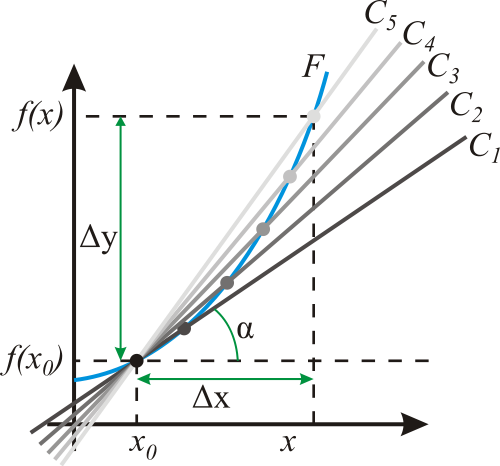
\includegraphics[scale=0.4]{immagini/matematica/derivata}
\caption{\label{img_derivata}Significato geometrico della derivata.}
\end{figure}

Com'è possibile? Dalla definizione (che dovreste ricordare) di velocità cioè:
\begin{equation}\label{mate_velmedia}
 v = \dfrac{s}{t} = \dfrac{\Delta x}{\Delta t}
\end{equation}
abbioamo che, quando l'intervallo di tempo diventa abbastanza piccolo, (ossia quando $\Delta t \to 0$) si ricava:
\begin{equation}
v(t)=\lim_{\Delta t\rightarrow 0} v_m(t,t+\Delta t)=\lim_{\Delta t\rightarrow 0} \frac{\Delta x}{\Delta t}(t)= \left. \frac{\ud x}{\ud t}\right|_t
\end{equation}
dove con $v_m(t, t+ \Delta t)$ indichiamo la velocità media definita come in \ref{mate_velmedia} nell'intervallo $(t, t+\Delta t)$.

Inoltre, come si vede dalla figura \ref{img_derivata}, la derivata, essendo il limite del rapporto incrementale, 
non è nient'altro che il coefficiente angolare della retta tangente alla funzione nel punto $x=x_0$.

Abbiamo quindi che la retta tangente è un ottimo modo per approssimare una funzione in un intorno di un suo punto,
infatti possiamo scrivere:

\begin{equation}\label{first_order}
x(t) \approx x(t_0) + v(t_0)t
\end{equation}

Nel caso di moto rettilineo uniforme la \ref{first_order} è una relazione esatta (non è un'approssimazione).

\subsection{Derivate parziali e derivate direzionali}

Naturalmente la situazione si complica quando si passa da una dimensione, ossia dal moto lungo una retta, descritto da $x(t)$ 
a più dimensioni ($2$ nel piano, $3$ nello spazio), in questo caso possiamo definire la derivata parziale e la derivata 
direzionale: strumenti che generalizzano il concetto di derivata a funzioni di più variabili.

\begin{Def}{Derivata parziale}
Consideriamo una funzione di $n$ variabili $f(\vec{x})= f(x_1, x_2,\ldots,x_n)~:~E\to\mathbb{R}$. Si definisce derivata parziale di $f$ in $\vec{x}\in E$, 
rispetto alla variabile k-esima $x_k$, il limite, se esiste finito, di:
\begin{equation}
    \frac{\partial f(\vec{x})}{\partial x_k}=\lim_{h\to 0}\frac{f(x_1,x_2,\ldots,x_k+h,\ldots,x_n)-f(x_1,x_2,\ldots,x_n)}{h} 
\end{equation} 
\end{Def}

La derivata direzionale di una funzione scalare è la derivata fatta lungo una direzione definita da un vettore (di modulo unitario):
\[ \vec{u} = (u_1, \ldots, u_n) \]
ed è la funzione definita dal limite:
\begin{equation}
D_{\vec{u}}{f}(\vec{x}) = \lim_{h \rightarrow 0^+}{\frac{f(\vec{x} + h\vec{u}) - f(\vec{x})}{h}}.
\end{equation}

\section{Cinematica}

Richiamiamo nel seguito alcuni concetti fondamentali di cinematica: posizione, spostamento, velocità, accelerazione.

\subsection{\index{posizione}Vettore posizione}
\begin{Def}[vettore posizione]
Fissato un sistema di riferimento cartesiano\footnote{per semplicità quasi sempre si parlerà del piano piuttosto che dello spazio, ma i risultati sono del tutto analoghi} 
$xOy$ il vettore che congiunge l'origine con un punto $P$ è il \index{vettore!posizione}vettore posizione $\ve r$ che individua $P$ in quel sistema di riferimento.
\end{Def}

Quindi un punto nello spazio può essere individuato dando tre cordinate $(x_P, y_P, z_P)$, per esempio potete immaginare di dover indicare la 
posizione di un aereo, vi servono latitudine, longitudine, e quota.  È utile a questo punto introdurre i versori.

Poiché un corpo materiale può essere descritto da punto capace di spostarsi nel tempo $\ve r$ sarà funzione del tempo $\ve r=\ve r(t)$ e descriverà al variare del tempo tutte le posizioni occupate da $P$ 
cioè la sua traiettoria\index{traiettoria}.

\begin{figure}[htbp]
\centering
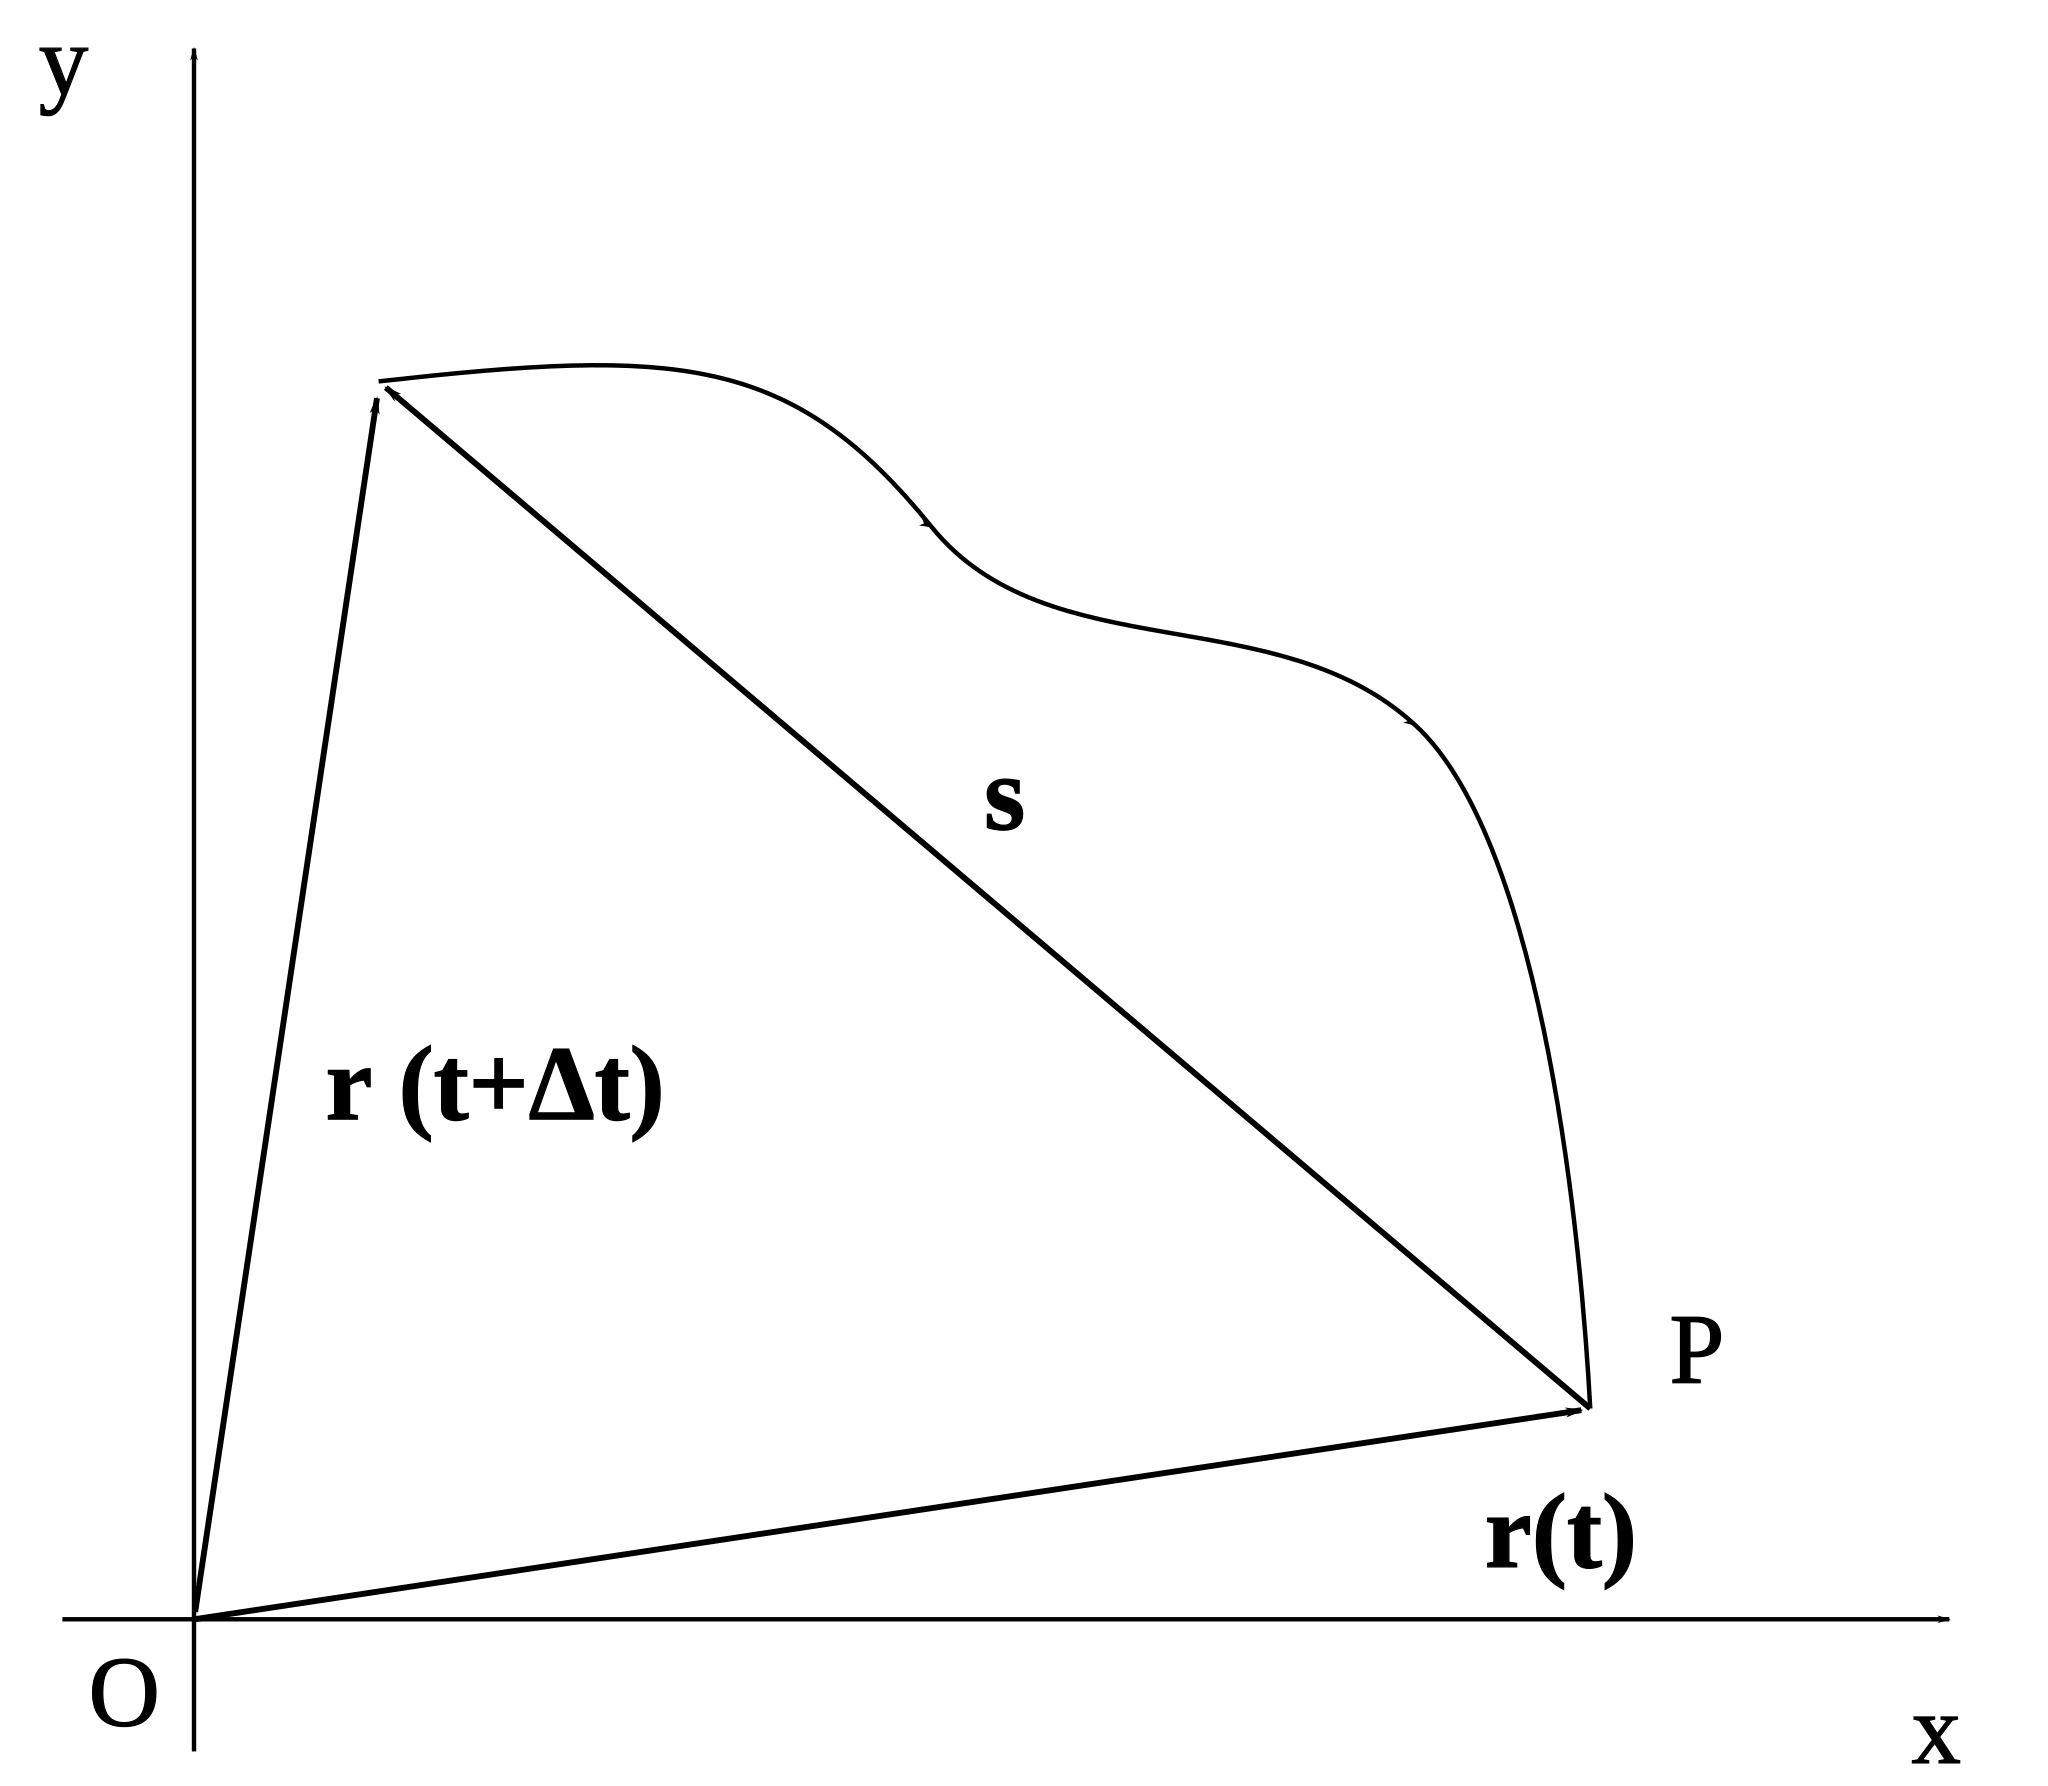
\includegraphics[scale=0.7]{immagini/matematica/vettore_posizione}
\caption{vettore posizione e spostamento.}
\end{figure}

\subsubsection{\index{versore}Versori e \index{coordinate}coordinate}
I versori sono vettori della base ortonormale di $\field{R}^3$ (lo spazio). In parole povere sono sono vettori di modulo unitario 
ortogonali (perpendicolari) a due a due. 
Solitamente si indicano con $\ver i$, $\ver j$ e $\ver k$ i versori applicati nell'origine, nella direzione degli assi cartesiani 
del sistema di riferimento. 

Le loro coordinate sono\footnote{quando si scrive che $\ve v=(a,b,c)$ l'uguaglianza significa che che fissata una base il 
vettore è rappresentato dalle sue coordinate $(a,b,c)$, ma vettori e coordinate non sono la stessa cosa, per esempio 
se si fa un cambiamento di base il vettore non cambia, ma le sue coordinate sì.}:

\begin{equation}
\ver \imath=\left(\begin{array}{c} 1\\0\\0\\ \end{array}\right)\qquad
\ver \jmath=\left(\begin{array}{c} 0\\1\\0\\ \end{array}\right)\qquad
\ver k=\left(\begin{array}{c} 0\\0\\1\\ \end{array}\right)
\end{equation}

Poiché i versori formano una base ogni vettore può essere espresso come una loro combinazione lineare, i coefficienti sono le coordinate\footnote{come già accennato i due simboli di uguaglianza hanno significati diversi, il primo è una vera uguaglianza, il secondo vuol dire che fissata una base, il vettore è rappresentato da quelle coordinate.}:
\begin{equation}
\ve v=v_x\ve i+v_y\ve j+v_z\ve k=\left(
\begin{array}{c}
v_x\\v_y\\v_z\\
\end{array}\right)
\end{equation}

\subsubsection{\index{prodotto!scalare}Prodotto scalare}
Il prodotto scalare usato in fisica è il prodotto scalare canonico della geometria in $\field{R}^3$ rispetto alla base canonica 
$\{\ver i,\ver j,\ver k\}$:

\begin{equation}\label{prodotto_scalare}
\left(\ve{x},\ve{y}\right)=\ve{x}^T\cdot\ve{y}=(x_1y_1+x_2y_2+x_3y_3)
\end{equation}

Un altro modo per esprimerlo è:
\begin{equation}
p_s=|\ve a||\ve b| \cos \alpha
\end{equation}
con $\alpha$ l'angolo compreso tra i due vettori. Da qui si deduce che $\ver i \cdot \ver i=1$, $\ver i
\cdot \ver j=0$, ecc., che due vettori ortogonali hanno prodotto scalare nullo e che due vettori hanno 
prodotto scalare massimo quando sono paralleli.

\[p_s=\ve a \cdot \ve b=(a_x\ve i+a_y\ve j+a_z\ve k)\cdot(b_x\ve
i+b_y\ve j+b_z\ve k)=a_xb_x+a_yb_y+a_zb_z\]

In particolare il prodotto scalare può essere usato per definire la norma\index{norma} (o modulo) di un vettore:
\begin{equation}
||\ve a|| = \sqrt{\ve a \cdot \ve a} = \sqrt{(a_x)^2 + (a_y)^2 + (a_z)^2}
\end{equation}
fatto questo si definisce la distanza\index{distanza} tra due punti nel seguente modo:
\begin{equation}
d(\ve x, \ve y) = ||\ve x - \ve y||
\end{equation}

\subsection{\index{velocità}Vettore velocità}
Applicando la classica definizione:
\begin{equation}\label{vel}
 v = \dfrac{\Delta s}{\Delta t}
\end{equation}
al vettore posizione otteniamo la velocità (vettoriale) media del nostro punto.

\begin{Def}[\index{velocità!media}Velocità Media]
\begin{equation}\label{vel_media}
\ve v_m(t,t+\Delta t)=\frac{\Delta\ve r(t,t+\Delta t)}{\Delta
t}=\frac{1}{\Delta t}\{\Delta x\ve i+\Delta y\ve
j\}=\frac{\Delta x}{\Delta t}\ve i+\frac{\Delta y}{\Delta t}\ve
j 
\end{equation}
\end{Def}

Facendo il limite dell'equazione \ref{vel_media} per $t \to 0$ abbiamo:
\begin{Def}[\index{velocità!istantanea}Velocità Istantanea]
\begin{equation}
\ve v(t)=\lim_{\Delta t\rightarrow 0}\ve v_m(t,t+\Delta t)=\lim_{\Delta t\rightarrow 0} \frac{\Delta\ve r}{\Delta t}(t)={\left.\frac{\ud \ve r}{\ud t}\right|_t}=\left.\frac{\ud x}{\ud t}\right|_t\ve i+\left.\frac{\ud y}{\ud t}\right|_t\ve j
\end{equation}
\end{Def}

\subsection{\index{accelerazione}Vettore accelerazione}
Allo stesso modo possiamo ottenere la definizione di accelerazione istantanea:
\begin{Def}[accelerazione istantanea]
\begin{equation}
 \ve a=\frac{\ud \ve v}{\ud t}={\frac{\ud^2 \ve r}{\ud t^2}}
\end{equation}
\end{Def}

Abbiamo quindi riformulato tutte le definizioni utilizzando il concetto di derivata.

\section[Moto rettilineo uniforme]{\index{moto!rettilineo uniforme}Moto rettilineo uniforme}
Usiamo sempre condizioni iniziali implicite, del tipo $t_0=0$, $\ve r(0)=\ve r_0$, $\ve v(0)=\ve v_0$.
\begin{Def}[moto rettilineo uniforme]
\[\ve v=\overrightarrow\const\]
\end{Def}
\[\ud\ve r=\ve v\,\ud t\qquad\int_{\ve r_0}^{\ve r}\ud\ve r=\int_0^t\ve v\,\ud t \qquad \ve r-\ve r_0=\ve v t\]
\begin{eqimp}{equation}
\ve r=\ve v t+\ve r_0
\end{eqimp}
\section{\index{moto!uniformemente accelerato}Moto uniformemente accelerato}
\begin{Def}[moto uniformemente accelerato]
\[\ve a=\overrightarrow{\const}\]
\end{Def}
\[\ve a\,\ud t=\ud \ve v\qquad\int_0^t\ve a\,\ud t=\int_{\ve v_0}^{\ve v}\ud \ve v\qquad\ve a t=\ve v-\ve v_0\]
\begin{eqimp}{equation}
\ve v=\ve a t+\ve v_0
\label{vt_01}
\end{eqimp}
\[\ve v=\ve a t+\ve v_0=\frac{\ud \ve r}{\ud t}\]
\[\ud \ve r=\left(\ve a t+\ve v_0\right)\ud t\qquad\int_{\ve r_0}^{\ve r}\ud \ve r=\int_0^t\left(\ve a t+\ve v_0\right)\ud t\qquad\ve r-\ve r_0=\frac{1}{2}\ve a t^2+\ve v_0 t\]
\begin{eqimp}{equation}
\ve r=\frac{1}{2}\ve a t^2+\ve v_0 t+\ve r_0
\label{vt_02}
\end{eqimp}


\chapter{Alcuni richiami di relatività galileiana}

La fisica classica pre-relativistica postulava l'esistenza di spazio e tempo assoluti, che avevano cioè valore indipendentemente 
dal sistema di riferimento utilizzato e che si basavano sulla misurazione di spazi e tempi\footnote{sarebbe più preciso dire lunghezze,
ovvero distanze tra due punti e intervalli temporali, ovvero durate.} uguali in qualunque sistema di riferimento.
In particolare, sia la teoria della relatività galileiana, sia la più completa teoria dinamica di Newton prevedevano 
l'esistenza di un sistema di riferimento inerziale al quale potevano essere ricondotti tutti gli altri attraverso 
le trasformazioni di Galileo. Tale sistema era solitamente identificato con quello delle stelle fisse.

In base a questi principi, qualunque osservazione compiuta in un sistema di riferimento inerziale conserva la misura delle lunghezze 
(per esempio di un regolo) così come gli intervalli di tempo (tra due eventi, come per esempio l'accensione di due lampadine). 
Allo stesso modo, in meccanica classica, due eventi simultanei in un sistema di riferimento (cioè con la stessa coordinata temporale) 
lo sono in ogni sistema di riferimento inerziale. Questo fatto trova il suo riscontro nelle trasformazioni galileiane, rispetto 
alle quali le leggi di Newton presentano una invarianza in forma.

\section{L'osservatore in relatività galileiana}

La concezione newtoniana di osservatore è basata sulla nozione di corpo
rigido (tipica nozione della geometria euclidea proveniente dalla fisica terrestre). 
Inizialmente un osservatore newtoniano è una piccola piattaforma
rigida, che costituisce il supporto dell’osservatore e che definisce il concetto
di localizzazione, nel senso che un evento avviene in un punto di tale piattaforma. 
In ogni punto della piattaforma è situato un orologio in quiete. In
breve, si dice che un osservatore newtoniano è una rete di orologi posti ai
vertici di un reticolato di regoli rigidi.

\begin{figure}[htbp]
  \centering
  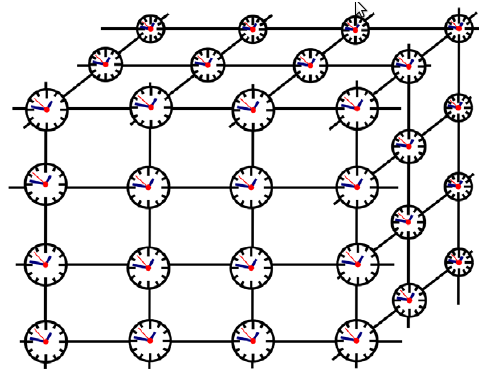
\includegraphics[scale=0.5]{immagini/galileo/oss_newton}
  \caption{Un osservatore come un reticolo di regoli e orologi.}
\end{figure}

In questa definizione si ammette tacitamente (e dal punto di vista matematico questa 
è un’ipotesi topologica sulla struttura dello spaziotempo) che tale reticolato possa 
essere esteso indefinitamente in tutte le direzioni (per questo si parla di coordinate globali), 
e che per le misure spaziali tra punti in quiete rispetto ai reticolati valgano le regole della geometria euclidea.

Per completare la definizione dell’osservatore newtoniano, bisogna infine
sincronizzare gli orologi posti nei diversi punti del reticolato: possiamo pensare 
che ogni punto abbia un suo piccolo ``laboratorio'', e bisogna fare in
modo che tutti questi ``laboratori'' siano sincronizzati. 
Il processo di sincronizzazione può essere fatto, ad esempio, per trasporto di un orologio campione,
e qui ipotizziamo tacitamente che la sincronizzazione non dipenda dal
trasporto e che orologi sincronizzati rimangano sincronizzati.

Il processo di sincronizzazione definisce il concetto di tempo relativo
all’osservatore, definito come il tempo misurato dall’orologio - in quiete
(rispetto alla piattaforma dell’osservatore) e sincronizzato nella rete di orologi
- nel punto in cui avviene l’evento. E chiaro che questa nozione ha significato
solo se gli orologi sono stati precedentemente sincronizzati.

\subsection{Gli assiomi della relaitività galileiana}

Definito il singolo osservatore come un sistema di coordinate globali sullo
spaziotempo (dove l’aggettivo ``globali'' rende conto del fatto che ogni evento
pu` essere localizzato poiché la piattaforma è estendibile all’infinito), rimane
da fare il confronto tra i diversi osservatori, il che equivale a porsi il problema
di un cambio di coordinate sullo spaziotempo.

Nella Relatività newtoniana si ammettono due assiomi, detti del tempo 
assoluto e dello spazio assoluto (in quest’ordine).

\subsubsection{L'assioma del tempo assoluto}
L'assioma del tempo assoluto afferma il carattere invariantivo delle durate, cioè delle differenze di tempo:
gli intervalli temporali tra due eventi misurati da due diversi osservatori newtoniani in moto relativo 
coincidono sempre, indipendentemente dalla natura del moto relativo questo vale, ad esempio, anche per moti non inerziali. 

In particolare, eventi simultanei in un riferimento sono simultanei in ogni altro
riferimento: il concetto di simultaneità è dunque un concetto assoluto, nel senso che è una ``proprietà
 che non dipende dall'osservatore - infatti la Relatività è lo studio di ciò che \textbf{non} 
dipende dagli osservatori a partire da ciò che dipende da tali osservatori. Questo contraddice in maniera totale chi cerca
di riassumere la Relatività con ``tutto è relativo''.

Se il concetto di simultaneità è assoluto, la simultaneità è una relazione di equivalenza,
che determina una partizione nello spaziotempo in classi di equivalenza\footnote{Una relazione di equivalenza è una 
relazione che gode delle seguenti proprietà:
\begin{itemize}
 \item riflessività
 \item simmetria
 \item transitività
\end{itemize}
un evento $A$ è chiaramente simultaneo a sè stesso, la relazione di simultaneità tra due eventi è simmetrica, ovvero 
se $A$ è simultaneo a $B$ allora $B$ è simultaneo ad $A$ ed infine se $A$ e $B$ sono simultanei e $B$ e $C$ sono simultanei, 
allora anche $A$ e $C$ sono simultanei (proprietà transitiva).}, i cosiddetti piani di simultaneità relativi a ciascun istante.

\subsubsection{L'assioma dello spazio assoluto}

Consideriamo un treno in moto rettilineo uniforme, un osservatore A posto a terra e un osservatore B all’interno del
treno che lasci cadere una pallina in terra. E chiaro che per l’osservatore B, concepito come piattaforma,
 la coordinata ``orizzontale'' del punto di lancio 
corrisponderà a quella del punto di arrivo; viceversa, per l’osservatore A,
durante la caduta, la pallina avrà percorso orizzontalmente un certo spazio.

Chiaramente, quindi, non possiamo affermare che la distanza spaziale
tra ogni coppia di eventi è invariante, poichè tale affermazione sarebbe palesemente
falsa, ma dobbiamo prendere in considerazione solamente eventi simultanei.
L'assioma dello spazio assoluto, infatti, afferma che la distanza tra le localizzazioni 
spaziali di due eventi simultanei è invariante. 

Questo enunciato ha senso perché il concetto di simultaneità, in base al primo postulato, ha
carattere assoluto, pertanto è importante enunciare i due postulati in questo ordine.

Si può dare una forma più intuitiva a questo assioma mediante la nozione
di lunghezza di un corpo in movimento - per corpi in quiete valgono, come
già detto, le regole della geometria euclidea. Per definizione, la lunghezza di
un regolo in moto è la distanza tra una qualsiasi coppia di punti in quiete
nella piattaforma che allo stesso istante nel tempo relativo coincidono con
gli estremi del regolo. Dunque la lunghezza di un corpo in moto è la distanza
tra due eventi simultanei, per esempio il passaggio di un regolo davanti a dei traguardi.

Con questo linguaggio si può dire che l'assioma dello spazio assoluto
afferma l’invarianza della lunghezza dei corpi in movimento.

\subsubsection{Il principio di relatività}
L’ultimo assioma è il \textbf{Principio di Relatività}, che ha una duplice valenza.
\begin{itemize}
 \item Puntando l'attenzione sugli osservatori, esso afferma una impossibilità,
nella fattispecie l’impossibilità, sulla base di esperienze meccaniche, di
selezionare un osservatore nella classe degli osservatori inerziali. Tutti
gli osservatori inerziali sono quindi equivalenti dal punto di vista della
meccanica;
\item dal punto di vista delle leggi fisiche, questo principio pone un vincolo
sulla forma delle leggi fisiche, che può diventare un
criterio per la loro selezione. Infatti, i fenomeni meccanici non
permettono di selezionare un osservatore inerziale privilegiato, perché
i fenomeni meccanici devono avvenire nello stesso identico modo in due diversi 
riferimenti inerziali, a parità di condizioni iniziali ed ambientali.
Ma i fenomeni fisici sono retti dalle leggi della fisica, e quindi tali leggi
devono essere le stesse in due diversi riferimenti inerziali. Infine, poiché
gli osservatori inerziali sono legati dalle leggi di Galileo, ne concludiamo
che le leggi della fisica devono essere invarianti in forma rispetto alle
trasformazioni galileiane (che vedremo fra poco);
\end{itemize}

Una formulazione equivalenti di questo asserto è che non esiste il ``moto assoluto'' che sarebbe, per l’appunto, il moto
rispetto all’osservatore privilegiato.

\section{\index{trasformazioni!di Galileo}Trasformazioni di Galileo}
Le trasformazioni di Galileo sono equazioni valide nella meccanica classica che consentono di descrivere le coordinate di un sistema rispetto 
alle di coordinate di un altro sistema che si muove di moto rettilineo uniforme rispetto al primo. 

Un sistema è detto inerziale se vale la prima legge di Newton: se su un corpo non agiscono forze o se la risultante delle forze è nulla allora esso mantiene il suo stato
di moto ovvero rimane in quiete se è fermo o si muove di moto rettilineo uniforme.

Se in un sistema è inerziale allora un altro sistema è inerziale se e solo se si muove di motto rettilineo uniforme rispetto al primo.

\begin{itemize}
 \item Primo osservatore ``fermo'':$\qquad O\quad\ve r(x,y,z)\quad\;\ve v\quad\;\ve a$
 \item Secondo osservatore in moto:$\quad O'\quad\!\ve r(x',y',z')\,'\quad\!\ve v\,'\quad\!\ve a\,'$
 \item In meccanica classica si assume: $t=t'$
 \item $\ve u$ velocità di trascinamento: \index{velocità!relativa}velocità di $O'$ rispetto ad $O$.
\end{itemize}

La terza assunzione, spesso lasciata implicita, si indica dicendo che nella relatività galileiana il tempo è assoluto.

\begin{figure}[htbp]
  \centering
  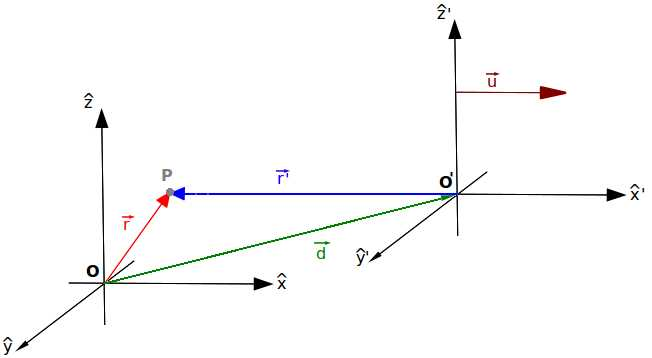
\includegraphics[scale=0.5]{immagini/galileo/sistemi}
  \caption{Cambio di coordinate tra sistemi inerziali.}
\end{figure}

Troviamo che valgono le seguenti leggi di trasformazione:
\begin{legge}
\begin{equation}\label{cambio_sis}
\ve r(t)=\overrightarrow{\left(O'-O\right)}+\ve r\,'= \ve d +\ve r = \ve u t+\ve r\,' 
\end{equation}
con $\ve d = \overrightarrow{\left(O'-O\right)} = \ve u t$ vettore di separazione tra i due sistemi.
\end{legge}
\begin{legge}[composizione delle velocità]
\index{composizione delle velocità}
\begin{equation}\label{cambio_vel}
\ve v=\frac{\ud\ve r}{\ud t}=\frac{\ud}{\ud t}\left(\ve u
t+\ve r\,'\right)=\frac{d}{\ud t}\left(\ve u
t\right)+\frac{\ud\ve r\,'}{\ud t}=\ve u+\frac{\ud\ve r\,'}{\ud
t'}=\ve u+\ve v\,' 
\end{equation}
usando la \ref{cambio_sis} si ottiene la \ref{cambio_vel}.
\end{legge}
\begin{legge}[invarianza dell'accelerazione]
\begin{equation}
\ve a=\frac{\ud \ve v}{\ud t}=\frac{\ud}{\ud t}(\ve u+\ve
v\,')=0+\frac{\ud \ve v\,'}{\ud t}=\frac{\ud \ve v\,'}{\ud
t'}=\ve a' 
\end{equation}
Concludiamo quindi che l'accelerazione è invariante: sistemi di riferimento diversi, ma inerziali misurano la stessa accelerazione 
per un corpo.
\end{legge}

Riassiumiano di seguito le trasformazioni di Galileo:
\begin{equation}\label{trasformazioni_galileo}
\left\{\begin{array}{ll}
\ve r=\ve r\,'+\ve u t&\\
\ve v=\ve u+\ve v\,'&\text{somma delle velocità}\\
\ve a=\ve a\,'&\text{invarianza dell'accelerazione}\\
t=t'&\text{ipotesi del tempo assoluto}\\
\end{array}\right. 
\end{equation}
In questo senso non esiste un sistema di riferimento privilegiato, ma le descrizione della fisica è equivalente in ogni sistema che si
muova di moto rettilineo uniforme (ovvero che sia inerziale) rispetto ad un altro. Il problema di questo approccio è il fatto che
è necessario assumere che esista almeno un sistema inerziale dal quale (con le trasformazioni di galieleo) si possano trovare tutti
gli altri. Questo sistema (il sistema ``fermo'') è quello delle stelle fisse.
\begin{Es}[lancio del sasso]
 Consideriamo due sistemi inerziali $O$ e $O'$. $O$ veda $O'$ muoversi lungo l'asse $x$ con velocità $\ve w$. Siano gli assi $y$ e $z$ uguali nei due sistemi. $O$ lancia un sasso verso l'alto, le equazioni del moto per il sasso visto da $O$ sono:
 \begin{gather*}
  x(t) = x_0\\
  y(t) = -\frac{1}{2}gt^2 + v_0 t
 \end{gather*}
 la traiettoria in questo caso è un segmento verticale con gli estremi in $(x_0,0)$ e $(x_0,\frac{v_0^2}{2g})$. Nel sistema $O'$ invece questo moto diventa:
 \begin{gather*}
  x'(t) = x(t) - w t = x_0 - wt\\
  y(t) = -\frac{1}{2}gt^2 + v_0 t
 \end{gather*}
 si noti che $v_0$ è sempre lo stesso nei due sistemi. Eliminando il tempo: $t = (x_0-x') /w$ si ottiene l'equazione di una parabola il cui vertice è ad una altezza uguale a quella nel sistema di $O$.
\end{Es}

\subsection{Rotazioni\index{rotazione}}

All'interno delle trasformazioni di Galileo possiamo annoverare anche le rotazioni.

In due dimensioni, una rotazione è una trasformazione $R(\theta)$, 
che dipende da un angolo $\theta$, e che trasforma il vettore $(x, y)$ in
\begin{equation}\label{rotazione}
\left\{\begin{array}{ll}
x'=x\cos\theta-y\sin\theta \\
y'=x\sin\theta+y\cos\theta
\end{array}\right. 
\end{equation}

Usando la moltiplicazione di matrici la rotazione può essere descritta così:
\begin{equation}
\begin{bmatrix} x' \\ y' \end{bmatrix} =
\begin{bmatrix} \cos \theta & -\sin \theta \\ \sin \theta & \cos \theta \end{bmatrix} 
\begin{bmatrix} x \\ y \end{bmatrix}
\end{equation}

La matrice quadrata presente in questa espressione è una matrice ortonormale di rango due. 
Questa trasformazione è chiamata ``rotazione antioraria'' di angolo $\theta$ intorno all'origine.
La matrice $2 \times 2$ che descrive la rotazione è spesso chiamata matrice di rotazione di angolo $\theta$

Se ora specializziamo la \ref{rotazione} per un angolo di $\theta = \frac{\pi}{6} = 30\degree$ abbiamo:
\begin{equation}\label{rotazione}
\left\{\begin{array}{ll}
x'=\dfrac{\sqrt{3}}{2}x-\dfrac{1}{2}y\\
y'=\dfrac{1}{2}x+\dfrac{\sqrt{3}}{2}y
\end{array}\right. 
\end{equation}
\begin{figure}[htbp]
  \centering
  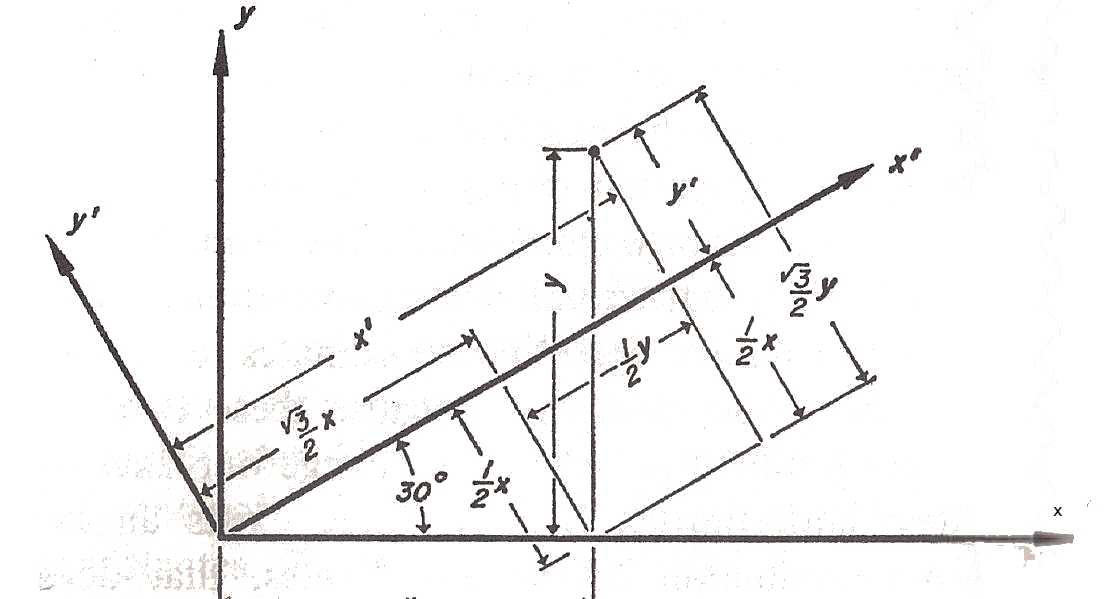
\includegraphics[scale=0.25]{immagini/galileo/rotaz}
  \caption{\label{Irotazionepi30}Una rotazione di $\dfrac{\pi}{3}$.}
\end{figure}

da confrontare con la figura \ref{Irotazionepi30}.

\section{Invarianza e covarianza\index{invarianza}\index{covarianza}}
Una grandezza si dice invariante se è numericamente uguale alla sua trasformata, cioè $x=T(x)=x'$.
Nelle trasformazioni di Galileo l'accelerazione è invariante rispetto alla trasformazione che trasforma le coordinate di $O$
in quelle di $O'$. Nella relatività galileiana la lunghezza è invariante, nella relatività ristretta no.

Una legge si dice covariante se la sua espressione è uguale alla sua trasformata, cioè $f(x)=T(f(x))$.

Concludiamo quindi che le leggi della dinamica ed in particolare la seconda legge di Newtown:
\begin{equation}\label{seconda_newton}
 \ve F = m \ve a 
\end{equation}
è invariante. Cioè, dato che tutti gli osservatori misureranno la stessa accelerazione $\ve a$, tutti concorderanno con 
\ref{seconda_newton}

Un altro esempio di oggetto invariante e che ci tornerà utile dopo è la distanza tra due punti quando si ruota o trasla 
il sistema di riferimento, abbiamo già visto com'è definita la distanza precedentemente.
Prendendo la distanza di un punto $P$ di coordinate $(x,y)$ indicato da un vettore $\ve P$, 
la sua distanza (al quadrato) dall'origine si scrive:
\begin{equation}\label{distanza_galileo}
 ||\ve P|| = x^2 + y^2 = s^2
\end{equation}

Se ruotiamo il sistema di riferimento abbiamo:
\begin{figure}[htbp]
  \centering
  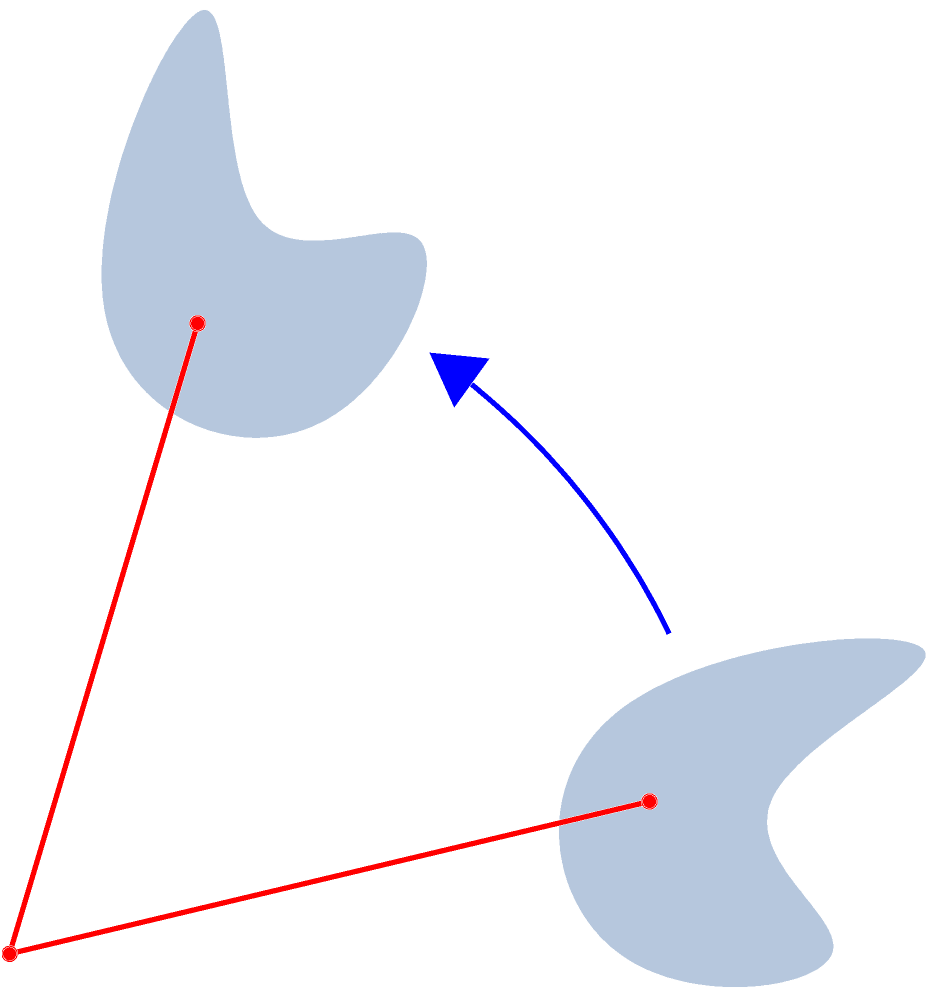
\includegraphics[scale=0.05]{immagini/galileo/Rotation_illustration}
  \caption{Rotazione antioraria nel piano.}
\end{figure}

Se sostituiamo \ref{rotazione} in \ref{distanza_galileo} abbiamo:
\begin{equation}
\begin{split}
s^2 &= {x'}^2 + {y'}^2 = \\
&= \left[\left(\dfrac{\sqrt{3}}{2}x-\dfrac{1}{2}y\right)^2 + \left(\dfrac{1}{2}x+\dfrac{\sqrt{3}}{2}y\right)^2\right] =\\
&= 4\dfrac{x^2 + y^2}{4} = x^2 +y^2
\end{split}
\end{equation}

e vediamo la quantità $s^2$ definita come sopra è invariante.
\chapter{La crisi della meccanica classica}

Il principio di equivalenza degli osservatori inerziali è rotto dalla scoperta di
Maxwell\footnote{James Clerk Maxwell (1831-1879), fisico scozzese le cui equazioni, a lui successivamente intitolate, mostrarono
la natura elettromagnetica della luce.} che la luce è un'onda elettromagnetica. Come tutte le onde fino ad allora note, 
si postulò che essa doveva propagarsi in un mezzo, detto etere.
A questo proposito Hermann Bondi scrisse\footnote{Hermann Bondi, La relatività e il senso comune, Zanichelli, pp. 36-37}:
\begin{quotation}
L'etere serviva a uno scopo, e a uno solo: rendere conto della propragazione della luce, 
essere per la luce ciò che l'aria è per il suono.
Ma l'aria può venir pesata, può venir messa in moto, può venir pompata fuori di un recipiente 
o può venir messa sotto pressione in esso; nulla di tutto ciò può essere fatto con questo 
ipotetico etere. [...]
Quindi l'etere non ha che una proprietà: aiuta a costruire una analogia tra propagazione della luce 
e propagazione del suono; [...] una falsa analogia. 
\end{quotation}

L'etere fornirebbe dunque un sistema di riferimento privilegiato, nel quale la luce si propaga 
isotropicamente con velocità $c$. In ogni altro riferimento, ad esempio nel riferimento terrestre,
la velocità della luce sarà necessariamente diversa a seconda della direzione di
propagazione. Si rese quindi necessario chiarire se l'etere fosse in moto rispetto alla Terra oppure no.

\section{Esperimento di Michelson--Morley\index{Michelson}\index{Morley}\index{esperimento!di Michelson--Morley|(}}

Se immaginiamo che l'etere sia solidale con il Sole abbiamo una evidente conseguenza: la Terra, essendo in moto 
rispetto all'etere e non trascinandolo, deve risentire di un ``vento d'etere''.
La luce quindi avrà una velocità diversa a seconda della sua direzione di moto, questo fatto può essere evidenziato 
con opportuni esperimenti che sfruttino il fenomeno dell'di interferenza. 
Michelson\footnote{Albert Abraham Michelson (1852-1931), 
primo scienziato americano a ricevere il premio Nobel (nel 1907); 
ha misurato la velocità della luce e ha inventato, sfruttando la
lunghezza d'onda della luce, un interferometro per misure precise.} e 
Morley\footnote{Edward W. Morley (1838-1923), chimico americano e collaboratore di Michelson nel
celeberrimo esperimento sull'etere.}, nel periodo 1882-1888, hanno cercato
di dedurre proprio da esperimenti di interferometria la velocità della terra
rispetto all'etere. Per fare ciò hanno creato un'apparecchiatura come quella
riportata in figura \ref{esperimentoMichelsonMorley}.

\begin{figure}[htbp]
\centering
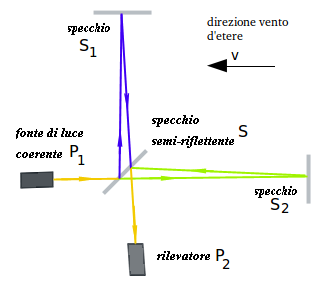
\includegraphics[scale=0.7]{immagini/michelson/Interferometro-Michelson}
\caption{\label{esperimentoMichelsonMorley}Esperimento di Michelson--Morley: Il dispositivo $P_1$ invia un fascio luminoso 
che viene parzialmente riflesso dallo specchio $S$.
Il raggio si spezza quindi in un raggio trasverso e in
un raggio longitudinale, riflessi rispettivamente dagli specchi $S_1$ e $S_2$ . I raggi
ritornano poi allo specchio $Q$ per confluire all'interfereometro $P_2$ . Dato che la
terra è in moto rispetto all'etere con una certa velocità $v$, l'interferometro $P_2$
dovrebbe rilevare frange d'interferenza.}
\end{figure}

Possiamo calcolare i tempi di percorrenza per i due diversi segnali luminosi. 
Contando che tali raggi hanno in comune il primo e l'ultimo tratto,
per il confronto ci basterà considerare il tratto trasverso (perpendicolare alla
velocità $v$, in verticale nel disegno) e il tratto longitudinale (parallelo a $v$, in
orizzontale nel disegno), entrambi di lunghezza $l$.


Nell'esperimento la luce proviene da una sorgente $P_1$, viene parzialmente riflessa da uno specchio 
semiargentato $S$ e contemporaneamente trasmessa. La luce quindi segue due cammini: $\text{I}$ e $\text{II}$; 
si riflette sugli specchi $S_1$ e $S_2$ e si riunisce in un raggio unico, prima di arrivare ad un'analizzatore. 
Le lunghezze dei percorsi dopo lo specchio $S$, $l_1$ e $l_2$ sono circa uguali, ma non uguali se riferite alla 
lunghezza d'onda della luce, quindi nell'analizzatore si dovrebbe vedere una figura d'interferenza. 
Si suppone che l'etere sia il sistema di riferimento assoluto e che l'apparecchio si muova con velocità $v$ 
verso destra, quindi si può supporre che sia l'etere a spostarsi verso sinistra con velocità $v$, il ``vento d'etere''. 
Non si considera il percorso dalla sorgente allo specchio $M$ e dallo specchio $M$ al rivelatore, in quanto i raggi viaggiano insieme. 
Il tempo per andare da $M$ a $M_1$ e tornare è:
\begin{equation}
\begin{split}
 t_1 = \frac{l_1}{c-v}+\frac{l_1}{c+v}=\frac{l_1(2c)}{c^2-v^2} = \\
    &= \frac{2c}{c^2}\frac{l_1}{1-\left(\frac{v}{c}\right)^2} = \frac{2l_1}{c}\frac{1}{1-\left(\frac{v}{c}\right)^2}
\end{split}
\end{equation}
Il percorso $\text{II}$ è ortogonale al vento d'etere, per semplicità si considera il punto di vista del vento d'etere:
\begin{figure}[htbp]
\centering
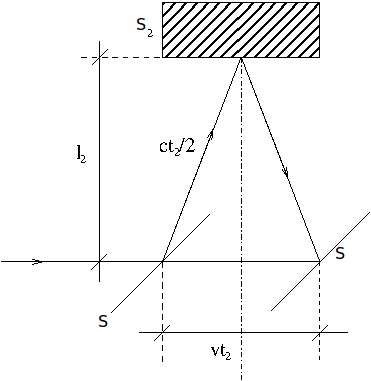
\includegraphics[scale=0.8]{immagini/michelson/Morley}
\caption{apparecchiatura vista dall'etere.}
\end{figure}

\parbox[]{\textwidth}{
\[s=2\sqrt{l_2^2+\left(\frac{vt_2}{2}\right)^2}=ct_2\]
\[l_2^2+\frac{v^2t_2^2}{4}=\frac{c^2t_2^2}{4}\qquad l_2^2=\frac{1}{4}\left(c^2-v^2\right)t_2^2\]
\[t_2=\frac{2l_2}{\sqrt{c^2-v^2}}=\frac{2l_2}{c}\frac{1}{\sqrt{1-\left(\frac{v}{c}\right)^2}}\]
}
La differenza di tempo dei due cammini è:
\[\Delta t=t_2-t_1=\frac{2}{c}\left\{\frac{l_2}{\sqrt{1-\left(\frac{v}{c}\right)^2}}-\frac{l_1}{1-\left(\frac{v}{c}\right)^2}\right\}\]
si osserva quindi una figura di interferenza. Se l'apparecchiatura viene ruotata di $90^\circ$ $l_1$ e $l_2$ si invertono:
\[\Delta t'={t_2}'-{t_1}'=\frac{2}{c}\left\{\frac{l_2}{{1-\left(\frac{v}{c}\right)^2}}-\frac{l_1}{\sqrt{1-\left(\frac{v}{c}\right)^2}}\right\}\]

\parbox[]{\textwidth}{
Si dovrebbe osservare una figura di interferenza diversa:
\begin{align*}
\Delta=&\Delta t'-\Delta t=\frac{2}{c}\left\{\frac{l_1+l_2}{{1-\left(\frac{v}{c}\right)^2}}-\frac{l_1+l_2}{\sqrt{1-\left(\frac{v}{c}\right)^2}}\right\}\\
=&\frac{2}{c}(l_1+l_2)\left\{1+\left(\frac{v}{c}\right)^2+\ldots-\left(1+\frac{1}{2}\left(\frac{v}{c}\right)^2\right)\right\}\\
\simeq&\frac{2}{c}(l_1+l_2)\frac{1}{2}\left(\frac{v}{c}\right)^2=\frac{l_1+l_2}{c}\left(\frac{v}{c}\right)^2\end{align*}
}
Con più riflessioni si riesce ad avere $l_1+l_2=\SI{20}{\metre}$, considerando il Sole come riferimento assoluto si ha $v=\SI{30}{\kilo\meter\per\second}$ e $\lambda=\SI{500E-9}{\metre}$.
Il numero di frange che scorrono dovrebbe essere:
\[\Delta N=\frac{\Delta}{T}=\frac{l_1+l_2}{\lambda}\left(\frac{v}{c}\right)^2\simeq 0.4\]
La sensibilità dello strumento era $\Delta N=0.01$. Se ci fosse stato l'etere con quella velocità sarebbe stato osservato. La ricerca dell'etere ripetuta in più mesi 
dell'anno, di giorno e di notte, usando luce solare, stellare ed artificiale, con dispositivi diversi, 
usando bracci diversi, telescopi o osservando fenomeni elettrici diede risultato negativo. 
Nel 1907 Michelson venne insignito del premio Nobel per la fisica.
\index{esperimento!di Michelson--Morley|)}

La coincidenza delle due durate può essere spiegata ripetendo formalmente i
calcoli con l'accortezza di indicare le distanze longitudinali e trasversali con
due simboli diversi (rispettivamente $l_{\parallel}$ e $l_{\bot}$). Troviamo che:
\begin{equation}
 T_{\bot} = \frac{2}{c}\dfrac{l_{\bot}}{\sqrt{1 - \frac{v^2}{c^2}}} = \frac{2}{c}\dfrac{l_{\parallel}}{1 - \frac{v^2}{c^2}} = T_{\parallel}
\end{equation}

L'esperienza di Michelson e Morley mostra che $T_{\parallel} = T_{\bot}$, e tale risultato si
spiega se ammettiamo che ovvero che $l_{\parallel} < l_{\bot}$ . Fitzgerald, nel 1892, 
concluse che il moto rispetto all'etere deve quindi comportare un fenomeno di distorsione a livello degli elettroni
(che compongono la materia, che interagiscono con forze elettromagnetiche
le quali riconoscono l'etere come osservatore privilegiato) per cui ogni regolo
si contrae nella direzione longitudinale (contrazione
delle lunghezze) della quantità:
\begin{equation}\label{gammaLorentz}
 \gamma = \dfrac{1}{\sqrt{1 - \frac{v^2}{c^2}}}
\end{equation}
la \ref{gammaLorentz} è detta fattore di Lorentz.

Se la spiegazione di Fitzgerald (che invoca un'interazione fino a quel tempo
sconosciuta tra materia ed etere responsabile del processo di contrazione)
da conto dell'esperimento nullo di Michelson e Morley, rimane aperto un secondo problema. 
L'esperimento di Michelson e Morley, infatti, è il primo
di una serie di esperimenti che mostrano che il campo elettromagnetico si
comporta nel laboratorio terrestre come previsto dalle leggi di Maxwell nell'etere. 
In sostanza, è come se le leggi di Maxwell valessero invariate in forma
sia nell'etere, sia nel laboratorio terrestre.

Nel 1895 Lorentz si pone dunque il problema di determinare matematicamente 
la più generale trasformazione di coordinate spaziotemporali che
lasci invariate in forma le equazioni di Maxwell. 

Il problema, tuttavia, era che ci si trovava di fronte ad un'incredibile coincidenza, la Terra
ritornava ad esere un sistema di riferimento privilegiato, ovvero quello in cui valgono le equazioni
di Maxwell. In un sistema di riferimento in moto rettilineo uniforme rispetto alla terra queste
equazioni diventano più complicate infatti esse non sono invarianti tra sistemi in modo. Dimostriamo questo
interessante fatto nel seguito. Per semplicità consideriamo come prototipo delle equazioni di Maxwell 
l'equazione delle onde  che in realtà è una conseguenza. 
Consideriamo il campo $E = E(x, t)$, in un universo bidimensionale. L'equazione delle onde è:
\begin{equation}
 \frac{1}{c^2} \dfrac{\partial^2 E}{\partial t^2} - \dfrac{\partial^2 E}{\partial x^2} = 0
\end{equation}

Mostriamo che tale equazione non è affatto invariante rispetto alle trasformazioni 
galileiane.

Ipotizzando infatti la trasformazione di coordinate
\begin{equation}
\left\{\begin{array}{ll}
x' = x - vt \\
t' = t
\end{array}\right.
\end{equation}

e la trasformazione della legge fisica $E (x', t') = E(x, t)$, otteniamo quindi che
$E (x - vt, t) = E(x, t)$ e dunque, calcolando le derivate parziali, si ha che:
\begin{equation}
 \left\{\begin{array}{ll}
  \dfrac{\partial E}{\partial t}(x,t) &= \dfrac{\partial E'}{\partial t'}(x-vt, t) - v \dfrac{\partial E'}{\partial x'}(x-vt,t) \\
  & \\
  \dfrac{\partial E}{\partial x}(x,t) &= \dfrac{\partial E'}{\partial x'}(x-vt, t)
 \end{array}\right.
\end{equation}

derivando nuovamente, sottintendendo i punti di calcolo delle derivate, si ha che:
\begin{equation}
 \left\{\begin{array}{ll}
  \dfrac{\partial^2 E}{\partial t^2} &= \dfrac{\partial^2 E'}{\partial t'^2} - 2v \dfrac{\partial^2 E'}{\partial x' \partial t'} + v^2  \dfrac{\partial^2 E'}{\partial x'^2} \\
  & \\
  \dfrac{\partial^2 E}{\partial x^2} &= \dfrac{\partial^2 E'}{\partial x'^2}
 \end{array}\right.
\end{equation}

Quindi, l'equazione delle onde nelle nuove coordinate assume la forma:
\begin{equation}
  \dfrac{1}{c^2}\dfrac{\partial^2 E}{\partial t'^2} - \dfrac{\partial^2 E'}{\partial x'^2} 
 - 2\dfrac{v}{c^2} \dfrac{\partial^2 E'}{\partial x' \partial t'} + \dfrac{v^2}{c^2}\dfrac{\partial^2 E'}{\partial x'^2} = 0
\end{equation}

Come si nota, tale forma è differente dalla precedente, poiché nella derivazione 
sono comparsi gli ultimi due termini che precedentemente non esistevano. 
L'equazione delle onde non è invariante in forma rispetto alle trasformazioni galileiane.
\chapter{Relatività speciale\index{relatività!speciale|(}\index{relatività!ristretta|see{speciale}}}
\minitoc

La cinematica sviluppata da Galileo e la meccanica sviluppata da Newton, che costituiscono le fondamenta della cosiddetta 
fisica classica, hanno riscosso enormi successi: ricordiamo in particolare la teoria copernicana del moto dei pianeti 
nel sistema solare e il ricorso alla cinematica per spiegare certe proprietà dei gas scoperte sperimentalmente, la 
teoria cinetica dei gas.
Rimangono tuttavia alcune categorie di fenomeni scoperti sperimentalmente che non possono essere interpretati alla luce 
di queste teorie classiche.

Nel 1905 Einstein espose la sua teoria della relatività ristretta partendo da un esperimento ideale da lui immaginato. 
A 16 anni, studiando la teoria dell' elettromagnetismo, aveva escogitato un paradosso: se vi muoveste alla velocità della luce 
parallelamente a un raggio di luce che viaggia nello spazio vuoto, osservereste un campo ``statico'' di elettricità e dei 
tracciati di campi magnetici. Ma Einstein ben sapeva che l'esistenza simultanea di campi elettrostatici e di campi magnetici 
violerebbe la teoria dell'elettromagnetismo. 
Bisognava far convivere le equazioni di Maxwell\index{Maxwell} con quelle di Newton.

Einstein si trovò di fronte a un' alternativa per risolvere questo paradosso: era sbagliata la teoria elettromagnetica
oppure lo era la cinematica classica, che ammette l'esistenza di un osservatore che può viaggiare solidale con un raggio luminoso? 

Einstein puntò sulla teoria elettromagnetica e andò in cerca di una variante alle teorie cinematiche di Newton e Galileo. 
Questa nuova cinematica, che sta alla base della relatività ristretta, vieta a qualsiasi osservatore (dotato di massa) 
di seguire solidarmente un raggio di luce.

Infine, vale la pena ricordare che quando i risultati sperimentali della fisica classica e della teoria della 
relatività appaiono in disaccordo, ha sempre vinto la relatività.

\section{Postulati di Einstein\index{Einstein!postulati di}\index{postulato!di Einstein}}
La teoria della relatività si fonda su due postulati che riportiamo qui di seguito:
\begin{post}[Principio di relatività speciale]
Tutte le leggi fisiche sono invarianti per traslazioni uniformi
\end{post}
\begin{post}[Invarianza della velocità della luce]
La velocità della luce nel vuoto è uguale in tutti i sistemi di riferimento
\end{post}

Dobbiamo trovare una la forma di una generica trasformazione che rispetti questi due postulati. 
Lo facciamo nella prossima sezione.

\subsection{Trasformate di Lorentz\index{trasformate!di Lorentz|(}\index{trasformazioni!di Lorentz|(}\index{Lorentz}}
Le trasformate i Lorentz sostituiscono le trasformate di Galileo della meccanica classica.
Un'altra caratteristica desiderabile per queste trasformazioni è che per velocità basse rispetto a quelle della luce 
le trasformate di Lorentz tendono a quelle di Galileo, infatti ci aspettiamo che la meccanica classica, che descrive così
bene il moto di treni, automobili, palle di cannone e altri oggetti ordinari, sia contenuta in questa teoria più estesa.
Ricaviamo nel seguito la forma esplicita di queste trasformazioni.

La funzione che trasforma le coordinate di un sistema di riferimento 
a quelle di un altro deve essere lineare. Un'applicazione si dice lineare se gode di due proprietà:
\begin{itemize}
 \item omogeneità: $f(\alpha \ve x) = \alpha f(\ve x)$, $\alpha \in \mathchar{R}$ 
 \item additività: $f(\ve x + \ve y) = f(\ve x) + f(\ve y)$
\end{itemize}
 
Infatti, immaginando che l'applicazione non sia lineare, per esempio: $x'=kx^2$, otteniamo dei risultati assurdi. 
Se mettessimo una sbarra tra $0$ e $1$ questa misura $\Delta x=1-0=1$, 
nel nuovo sistema di riferimento misura: $k\cdot 1^2-k\cdot 0^2=k$.
Se ora mettessimo la sbarra tra $2$ e $1$ nel primo sistema di riferimento misurerà ancora $1$, mentre nel secondo ù
si avrebbe $k(2^2-1^2)=3k$ ovvero spostando la sbarra nel secondo sistema di riferimento la sua lunghezza cambia: 
assurdo per l'ipotesi di omogeneità dello spazio; inoltre l'applicazione deve essere anche additiva, 
perché la lunghezza di due sbarre affiancate deve essere la somma dell'unica sbarra avente lunghezza 
uguale nel primo sistema di riferimento alla somma delle lunghezze delle due sbarre nel primo sistema di riferimento. 

Consideriamo il sistema di riferimento $Oxy$ fermo e $O'x'y'$ che si muove rispetto ad $O$ di moto rettilineo 
uniforme con velocità di trascinamento $u$ nella direzione dell'asse $x$ crescente. L'applicazione è lineare, 
quindi (in due dimensioni spaziali), in generale:
\[\left\{
\begin{array}{l}
x'=\lambda_{11}x+\lambda_{12}y+\lambda_{14}t\\
y'=\lambda_{21}x+\lambda_{22}y+\lambda_{24}t\\
t'=\lambda_{41}x+\lambda_{42}y+\lambda_{44}t\\\end{array}\right.
\]
Dove troviamo un sistema con 9 incognite. Facciamo alcune ipotesi aggiuntive:
\begin{itemize}
\item[-] al tempo $t=t'=0$ gli orologi coincidono e anche i sistemi di riferimento $O\equiv O'$, in particolare per $t=0$ e $x=0$ segue $x'=0$ cioè
\[x'=\lambda_{11}x+\lambda_{12}y+\lambda_{14}t\]
\[0=\lambda_{11}\cdot 0+\lambda_{12}y+\lambda_{14}\cdot 0\]
\[\lambda_{12}=0\]
\item[-] come sopra:
\[t'=\lambda_{41}x+\lambda_{42}y+\lambda_{44}t\]
\[0=0+\lambda_{42}y+0\]
\[\lambda_{42}=0\]
\item[-] la traslazione del sistema in moto è orizzontale, quindi $y'=0\Leftrightarrow y=0$ sempre.
\[\lambda_{21}=0\]
\[\lambda_{24}=0\]

\end{itemize}

Se mettiamo una sbarra verticalmente con un estremo in $O'$, questo misura che la lunghezza è $1$. 
La sbarra si muove con $O'$ e quindi questa è la lunghezza a riposo. Questa lunghezza a riposo dovrà essere uguale anche se è osservata da $O$. Mettiamo la sbarra ferma rispetto ad $O'$, quindi $O$ vede una lunghezza:
\[y=\frac{1}{\lambda_{22}}\]
mettiamo ora la sbarra ferma rispetto a $O$, $O'$ vede una lunghezza:
\[y'=\lambda_{22}\]
Le due situazioni sono simmetriche e quindi non esistendo un sistema privilegiato le due grandezze devono essere uguali:
\[\lambda_{22}=\frac{1}{\lambda_{22}}\qquad\lambda^2_{22}=1\]
Si scarta la soluzione negativa, in quanto si vuole che gli assi abbiano lo stesso verso.

\parbox[]{\textwidth}{
Seguiamo il moto dell'origine del sistema $O'$. Qui, per ogni istante:
\[x'=0\]
Per $O$ lo stesso moto è descritto da:
\[x=ut\qquad x-ut=0\]
Ci si aspetta allora un'equazione del tipo
\[x'=\lambda(x-ut)\]
}

A $t=0$, $O\equiv O'$, $t=t'$ scatta un'onda luminosa dalle origini, questa ha un fronte sferico con raggio $R$ e per il secondo principio di Einstein ha velocità $c$ uguale in tutti e due i sistemi. Il sistema $O'$ sta arrivando da sinistra, passa in coincidenza con $O$, si sincronizzano gli orologi e parte il fronte d'onda. I due osservatori osservano un fronte d'onda che ha centro nei propri sistemi di riferimento, anche se non sono più coincidenti:
\[x^2+y^2+z^2=R^2=(ct)^2\]
\[x'^2+y'^2+z'^2=R'^2=(ct')^2\]
\[x^2+y^2+z^2-ct^2=0=x'^2+y'^2+z'^2-(ct')^2\]
\[x^2-c^2t^2=x'^2-c^2t'^2=\lambda^2(x-ut)^2-c^2(\lambda_{41}x+\lambda_{44}t)^2=\]
\[=\lambda^2x^2+\lambda^2 u^2t^2-2\lambda^2 xut-c^2\lambda_{41}^2x^2-c^2\lambda_{44}^2t^2-2c^2\lambda_{41} x\lambda_{44} t\]
Risolvendo in $\lambda^2$, $\lambda_{41}^2$ e $\lambda_{44}^2$ si ottiene un sistema di tre incognite e tre equazioni:
\[\left\{
\begin{array}{l}
1=\lambda^2-c^2\lambda_{41}^2\\
-c^2=\lambda^2u^2-c^2\lambda_{44}^2\\
0=-2\lambda^2u-2c^2\lambda_{41}\lambda_{44}\\
\end{array}
\right.\quad \left\{
\begin{array}{l}
\lambda_{41}^2=\frac{\lambda^2-1}{c^2}\\
\lambda_{44}^2=\frac{c^2+\lambda^2u^2}{c^2}\\
-\lambda^2u=c^2\lambda_{41}\lambda_{44}\\

\end{array}\right.\]
Ci ricordiamo dell'ultima espressione che $\lambda_{41}\lambda_{44}<0$
\[\lambda^4u^2=c^4\lambda_{41}^2\lambda_{44}^2=c^4\frac{\lambda^2-1}{c^2}\frac{c^2+\lambda^2u^2}{c^2}=\]
\[=(\lambda^2-1)(c^2+\lambda^2u^2)=-c^2-\lambda^2u+\lambda^2c^2+\lambda^4u^2\]
\[0=-c^2-\lambda^2u^2+\lambda^2c^2\]
\[\lambda^2=\frac{c^2}{c^2-u^2}=\frac{1}{1+\frac{u^2}{c^2}}\]
\[\lambda=\dfrac{1}{\sqrt{1-\left(\dfrac{u}{c}\right)^2}}=\dfrac{1}{\sqrt{1-\beta^2}}=\gamma\]
\[\lambda_{41}^2=\frac{\lambda^2-1}{c^2}=\frac{\beta^2}{c^2(1-\beta^2)}\]
\[\lambda_{41}=\pm\frac{\beta}{c\sqrt{1-\beta^2}}\]
\[\lambda_{44}^2=\frac{c^2+\lambda^2u^2}{c^2}=\frac{1}{1-\beta^2}\]
\[\lambda_{44}=\pm\frac{1}{\sqrt{1-\beta^2}}\]
Diamo segno positivo a $\lambda_{44}$ e negativo a $\lambda_{41}$, in quanto se consideriamo un istante molto prossimo al momento della partenza allora $x\rightarrow 0$, $t'$ deve essere positivo (il tempo scorre nello stesso verso) e quindi $\lambda_{44}>0$.

Nei calcoli precedenti abbiamo definito le quantità:
\begin{equation}
\beta = \dfrac{v}{c} 
\end{equation}

\begin{equation}
 \gamma = \dfrac{1}{\sqrt{1-\beta^2}} = \dfrac{1}{\sqrt{1 - \frac{v^2}{c^2}}}
\end{equation}

Quindi alla fine le trasformazioni cercate sono le seguenti:
\begin{equation}
\left\{
\begin{array}{l}
x^\prime=\dfrac{x-vt}{\sqrt{1-\beta^2}}\\
y^\prime=y\\
z^\prime=z\\
t^\prime=\dfrac{t-\frac{\beta}{c}x}{\sqrt{1-\beta^2}}
\end{array}\right.
\end{equation}

\subsection{Trasformate di Lorentz e Galileo}
Verifichiamo che le trasformazioni trovate rispettano quel ``principio di corrispondenza'' accennato sopra, ovvero che la meccanica
classica e le trasformazioni di Galileo vengano riprodotte per velocità ``ordinarie'', questo equivale a dire che se $u\ll c$,
cioè se $\beta\rightarrow 0$ allora le trasformazioni di Lorentz si riducono a quelle di Galileo.
\[\left\{
\begin{array}{l}
x^\prime=\dfrac{x-vt}{\sqrt{1-\beta^2}}\\
y^\prime=y\\
z^\prime=z\\
t^\prime=\dfrac{t-\frac{\beta}{c}x}{\sqrt{1-\beta^2}}
\end{array}\right.
\quad \stackrel{\beta\rightarrow 0}{\longrightarrow} \quad
\left\{
\begin{array}{l}
x^\prime=x-ut\\
y'=y\\
z'=z\\
t'=t\\
\end{array}\right.\]
\index{trasformate!di Lorentz|)} \index{trasformazioni!di Lorentz|)}

\subsection{Le trasformazioni di Lorentz}
Lorentz ha quindi cercato una trasformazione di coordinate adatta per mantenere l’invarianza in forma delle equazioni di Maxwell. 
Riassumiamo le trasformazioni (riportando una sola dimensione spaziale):
\begin{equation}\label{Lorentz_riass}
  \left\{\begin{array}{ll}
   x' = \gamma \left(x - vt \right) \\
   t' = \gamma \left(t - \dfrac{v}{c^2}x \right)
  \end{array}\right.
\end{equation}

Come notiamo, Lorentz ha apportato due modifiche alle trasformazioni
di Fitzgerald. Ha lasciato invariata la contrazione delle lunghezze, ma ha
aggiunto una dilatazione dei tempi. Il fattore davanti a $t$ (inserito per
analogia) non bastava infatti per avere l’invarianza in forma: Lorentz ha
dovuto anche introdurre il termine $- \frac{v}{c^2} x$ (che è a tutti gli effetti un tempo)
nell'equazione dei tempi.

Con questa nuova trasformazione si verifica che:
\begin{equation}
\left\{
  \begin{array}{ll}
  \dfrac{\partial E}{\partial t} = - \gamma v \dfrac{\partial E'}{\partial x'} - \gamma \dfrac{\partial E'}{\partial t'} \\
  \dfrac{\partial E}{\partial x} = \gamma \dfrac{\partial E'}{\partial x'} - \dfrac{\gamma v}{c^2}\dfrac{\partial E'}{\partial t'}                
  \end{array}\right.
\end{equation}

e derivando nuovamente:
\begin{equation}
\left\{
  \begin{array}{ll}
  \dfrac{\partial^2 E}{\partial t^2} = - \gamma^2 v^2 \dfrac{\partial^2 E'}{\partial x'^2} - 2 \gamma v \dfrac{\partial^2 E'}{\partial x' \partial t'} + \gamma^2 \dfrac{\partial^2 E'}{\partial t'^2}\\
  \dfrac{\partial^2 E}{\partial x^2} = \gamma^2 \dfrac{\partial^2 E'}{\partial x'^2} - 2 \dfrac{\gamma^2 v}{c^2}\dfrac{\partial E'}{\partial x' \partial t'} + \dfrac{\gamma^2 v^2}{c^4}\dfrac{\partial E'}{\partial x' \partial t'}
  \end{array}\right.
\end{equation}
Le derivate miste si semplificano. Inoltre sapendo che sono verificate le seguenti identità:
\begin{equation}
\left\{
  \begin{array}{ll}
  \dfrac{v^2}{c^2 \left(1 - \frac{v^2}{c^2}\right)} - \dfrac{1}{\left(1 - \frac{v^2}{c^2}\right)} = -1 \\
  \dfrac{1}{c^2 \left(1 - \frac{v^2}{c^2}\right)} - \dfrac{v^2}{c^4 \left(1 - \frac{v^2}{c^2}\right)} = \dfrac{1}{c^2} \\
  \end{array}\right.
\end{equation}
otteniamo l’equazione delle onde nelle nuove coordinate:
\begin{equation}
 \frac{1}{c^2} \dfrac{\partial^2 E}{\partial t^2} - \dfrac{\partial^2 E}{\partial x^2} = 0
\end{equation}

equazione che ha conservato intatta la forma che aveva come conseguenza
delle equazioni di Maxwell. Le trasformazioni di Lorentz nascono proprio
per mantenere questa invarianza in forma.

\section{Effetti relativistici\index{effetti relativistici}}
In questa sezioni presenteremo alcuni particolari effetti relativistici che si allontanano dal ``senso comune'' e sono peculiari
della teoria della relatività, essi sono:
\begin{itemize}
 \item la contrazione delle lunghezze;
 \item la dilatazione dei tempi;
 \item la perdita del concetto di simultaneità assoluta;
 \item la composizione delle velocità;
\end{itemize}

\subsection{Contrazione delle lunghezze\index{contrazione delle lunghezze}}
\begin{figure}[htbp]
   \centering
   \includegraphics[scale=0.5]{immagini/relspec/beta_gamma}
   \caption{Variazione di $\gamma$ in funzione di $\beta$.}
\end{figure}
Consideriamo l'effetto delle trasformazioni di Lorentz sulla misura di lunghezze.
Posizioniamo un'asta con estremi $A$ e $B$ ferma rispetto ad $O'$, 
sistema di riferimento inerziale con velocità $u$ rispetto ad $O$.
$O$ misura nello stesso istante le posizione di $A$ e di $B$, quindi $t_A\equiv t_B$:
\[\left\{
\begin{array}{l}
x'_A=\frac{x_A-ut_A}{\sqrt{1-\beta^2}}\\
x'_B=\frac{x_B-ut_B}{\sqrt{1-\beta^2}}\\
\end{array}
\right.\]
\begin{align*}
l' &= x'_B-x'_A=\frac{x_B-x_A-ut_B+ut_A}{\sqrt{1-\beta^2}}= \\
&= \frac{x_B-x_A-u(t_B-t_A)}{\sqrt{1-\beta^2}}=\frac{x_B-x_A}{\sqrt{1-\beta^2}}\\
&=\gamma l
\end{align*}
Quindi abbiamo:
\begin{equation}
l=\frac{l'}{\gamma}
\end{equation}
Considerando che $0<\beta<1$ il che implica $\gamma>1$ si ha che $l<l'$, abbiamo che $O$ osserva un oggetto (in moto) 
la cui lunghezza è contratta rispetto alla lunghezza a riposo.

\subsection{Dilatazione dei tempi\index{dilatazione dei tempi}}
Consideriamo ora eventi osservati da $O'$ nello stesso spazio ($x'_A\equiv x'_B$) a distanza di tempo $\tau'=t'_B-t'_A$.
\[t'=\gamma\left(t-\frac{\beta}{c}x\right)\]
Per simmetria posso dire direttamente che:
\[t=\gamma\left(t'+\frac{\beta}{c}x'\right)\]
quindi abbiamo che:
\[t_A=\gamma\left(t'_A+\frac{\beta}{c}x'_A\right)\]
\[t_B=\gamma\left(t'_B+\frac{\beta}{c}x'_B\right)\]
e l'intervallo temporale tra i due eventi $\tau$ è dato da:
\begin{equation}
\tau=t_B-t_A=\gamma\left(t'_B-t'_A+\frac{\beta}{c}\left(x'_B-x'_A\right)\right)=\gamma\left(t'_B-t'_A\right)=\gamma\tau'
\end{equation}
Essendo $\gamma>1$ si ha che $\tau>\tau'$ cioè secondo $O$ il tempo misurato da $O'$ scorre più lentamente.

\begin{Es}[produzione e decadimento di mesoni $\pi^+$]
Se lanciamo un protone a colpire un altro protone fermo si può verificare la seguente ``reazione'':
\[p+p\rightarrow p+n+\pi^+\]
Durante la quale viene prodotto un mesone $\pi$ o pione. Questo decade nel seguente modo:
\[\pi^+ \rightarrow \mu ^+ + \nu_{\mu}\]

Se ci poniamo nel sistema di riferimento del mesone (ossia se lo cavalchiamo)
osserviamo un tempo di vita media $\tau'=\SI{1.88E-8}{\second}$. Il mesone ha rispetto al laboratorio $\beta=0.99$. Il laboratorio dalla distanza percorsa dal mesone calcola una vita media diversa:
\[\tau=\gamma\tau'=\frac{\tau'}{\sqrt{1-\beta^2}}\simeq 7.1\tau'=\SI{1.3E-7}{\second} \]
La distanza percorsa dal mesone, prima di decadere, osservata dal laboratorio è quindi:
\[d=\tau u=\tau \beta c\simeq \SI{39}{\metre} \]
\end{Es}

\subsection{Perdita del concetto di simultaneità assoluta\index{simultaneità!}}

\begin{figure}[htbp]
   \centering
   \includegraphics[scale=0.2]{immagini/relspec/pistoleri}
   \caption{Due pistoleri relativistici.}
   \label{pistoleri}
\end{figure}

I due pistoleri (Fig.\@ \ref{pistoleri}) sparano quando la luce gli raggiunge. 
Essi sono in un sistema solidale con la luce e quindi vedono contemporaneamente la luce della lampadina. 
Per il capostazione ``fermo'' invece è il pistolero di sinistra ad essere investito per prima dalla luce, 
quindi il pistolero a destra muore, mentre quello di sinistra no.
Gli eventi simultanei per $O'$ non sono tali per $O$, bisogna rivedere il concetto di tempo assoluto.

\subsection{Composizione delle velocità\index{composzione delle velocità!relativistiche}}
Come si potrà immaginare la composizione delle velocità non segue più le trasformazioni di Galileo. 
Infatti, supponiamo di osservare una astronave che si muove con $v = 0.8 c$ rispetto ad un sistema di 
riferimento $O$ e contestualmente abbiamo un sistema di riferimento
$O'$ che si muove con velocità $u = 0.8 c$ in direzione opposta a quella dell'astronave.
Le trasformazioni di Galileo ci direbbero che l'astronave $O'$ misura per $O$ la velocità:
\[
 v' = v - u
\]
ossia $v' = 0.8c + 0.8c = 1.6c$ una velocità maggiore di quella della luce, ma questo è impossibile! È necessario
cambiare la legge di composizione delle velocità.

La velocità rimane sempre la derivata del vettore posizione: $v_x=\frac{\ud x}{\ud t}$, 
quindi andiamo a calcolare queste derivate nel sistema traslato per trovare le leggi di composizione delle velocità:
\begin{equation}\label{composizione_vel_x}
\begin{split}
  v'_{x'} &= \frac{\ud x'}{\ud t'}=\frac{\ud x'}{\ud t}\frac{\ud t}{\ud t'}=\frac{\ud x'}{\ud t}\dfrac{1}{\frac{\ud t'}{\ud t}}= \\
	  &= \gamma\left(\frac{\ud x}{\ud t}-u\right)\dfrac{1}{\gamma\left(1-\dfrac{\beta}{c}\dfrac{\ud x}{\ud t}\right)} = \dfrac{v_x-u}{1-\dfrac{\beta}{c}v_x}
\end{split}
\end{equation}
\begin{equation}\label{composizione_vel_y}
\begin{split}
  v'_{y'} &= \frac{\ud y'}{\ud t'}=\frac{\ud y}{\ud t'}=\frac{\ud y}{\ud t}\frac{\ud t}{\ud t'}=v_y\frac{1}{\frac{\ud t'}{\ud t}}= \\
	  &= \dfrac{v_y}{\gamma\left(1-\dfrac{\beta}{c}\dfrac{\ud x}{\ud t}\right)}=\dfrac{v_y\sqrt{1-\beta^2}}{1-\dfrac{\beta}{c}v_x}
\end{split}
\end{equation}
Un'analoga equazione vale per $v'_{z'}$ essendo come $v'_{y'}$ una velocità trasversa rispetto ad $u$.
\[\lim_{\beta\rightarrow 0}v'_{x'}=v_x-u\qquad \lim_{\beta\rightarrow 0} v'_{y'}=v_y\]
cioè la composizione delle velocità secondo Galileo.

\begin{Es}[risolviamo il problema precedente]
Nell'esempio di prima:
\[\begin{array}{ll}
   v_x = 0.8 c\\
   u = - 0.8 c
  \end{array}
\]
applicando la \ref{composizione_vel_x} abbiamo:
\[v'_x=\frac{v_x - u}{1-\frac{\beta}{c}v_x}=\frac{0.8c - (- 0.8c)}{1+\frac{0.8}{c}0.8c} \approx 0.98c\]
ossia $v'_x < c$, come ci aspettavamo.
\end{Es}

\begin{Es}[decadimento $\pi^0$]
$\pi^0$ decade con un decadimento elettromagnetico del tipo:
\[\pi^0\rightarrow \gamma\gamma\]
Per la conservazione della quantità di moto i due fotoni devono avere velocità opposte, $c$ misurate sia dal sistema del laboratorio ($O$) sia dal sistema in moto con il $\pi^0$, $O'$. Supponiamo che i fotoni si propaghino secondo l'asse $x$ e che il mesone si muovesse alla velocità $u$ verso destra rispetto ad $O$. Per Einstein la velocità dei due fotoni vista da $O$ e da $O'$ è uguale.
Per il fotone che va a destra:
\[v_x=\frac{v'_{x'}+u}{1+\frac{\beta}{c}v'_{x'}}=\frac{c+u}{1+\frac{u}{c^2}c}=c\]
Per l'altro:
\[v_x=\frac{-c+u}{1-\frac{u}{c^2}(-c)}=-c\]
\end{Es}

\section{Massa\index{massa!relativistica}}
Dalla conservazione della quantità di moto ricaviamo la massa relativistica.

\begin{Es}[quantità di moto classica vs relativistica]
\begin{figure}[htbp]
   \centering
   \includegraphics[scale=0.5]{immagini/relspec/massa_relat.png}
   \caption{Altri due pistoleri relativistici. I due pistoleri (identici) sono in moto relativo, armati di pistole identiche e con proiettili
identici.}
\end{figure}

Siano $O$ e $O'$ due osservatori dotati di due pistole identiche con proiettili identici. 
$O'$ si muove verso destra rispetto ad $O$ con velocità costante $\ve v$\footnote{Gli assi $x$ e $x'$ non coincidono, sono sfasati, 
ma questo conta poco perché considerando le velocità, cioè derivando, il problema scompare.}. 
$O'$ spara in direzione di $O$ cioè nel verso delle $y$ decrescenti. $O$ vede il suo proiettile con velocità:
\[\dot y'_{O'}=-v\qquad\dot{x'}_{O'}=0\]

Dove abbiamo indicato con un puntino la derivata rispetto al tempo ($\dot y = \dfrac{\partial y'}{\partial t'}$ è quindi una
velocità), con l'apice il fatto che è una quantità misurata dall'osservatore $O'$ e con il pedice che è il proiettile sparato da
$O'$.

$O$ vede il proiettile di $O'$ con velocità:
\[\dot y_{O'}=\frac{\dot y'_{O'}\sqrt{1-\beta^2}}{1-\frac{\beta}{c}\dot x'_{O'}}=-\sqrt{1-\frac{u^2}{c^2}}v\]

$O$ spara a $O'$ nel verso delle $y$ crescenti e misura la velocità del proiettile:
\[\dot y_{O}=v\qquad \dot x_{O}=0\]
e $O'$ vede il proiettile di $O$ con:
\[\dot y'_{O}=\sqrt{1-\frac{u^2}{c^2}}v\]

La quantità di moto si deve conservare e sappiamo che prima che i due pistoleri sparassero era uguale a zero quindi abbiamo che 
l'osservatore $O$ descrive il sistema con la seguete equazione di conservazione della quantità di moto:
\[m_{O}U+m_{O'}\dot y_{O'}=0\]
\[m_{O'}=\frac{m_O v}{\sqrt{1-\frac{u^2}{c^2}}v}=\frac{m_O}{\sqrt{1-\frac{u^2}{c^2}}}\]

Vediamo che entrambi gli osservatori concordano sulla seguente osservazione: se ciascuno degli osservatori indica la massa del proiettile con la quantità $m_0$ (che, per ragioni che saranno evidenti nelle
  prossime righe è detta ``massa a riposo''. Ossia:
\begin{itemize}
 \item $O: m_{O} = m_0$;
 \item $O': m_{O'} = m_0$;
\end{itemize}
la massa del proiettile in moto (indicata semplicemente con $m$) diventa:
\[m=\frac{m_0}{\sqrt{1-\beta^2}}=\gamma m_0\]
Vediamo che la massa di una particella misurata da un'osservatore in moto varia con la velocità del moto relativo e in varticole se $v$ 
diventa prossimo a $c$ abbiamo che:
\[\beta\rightarrow 1\Rightarrow m\rightarrow +\infty\]
\end{Es}

\section{Quantità di moto\index{quantità di moto!relativistica}}
\[p=mv=\frac{m_0}{\sqrt{1-\beta^2}}\beta c=\gamma m_0 v\]
$\beta$ della particella. Con questa nuova definizione di quantità di moto essa si conserva ancora, anche in contesto relativistico.
\[\beta\rightarrow 1\Rightarrow p\rightarrow +\infty\]

\begin{Es}[quantità di moto classica vs relativistica]
\begin{figure}[htbp]
   \centering
   \includegraphics[scale=0.5]{immagini/relspec/Q_rel1}
   \caption{(a) prima dell'urto; (b) dopo l'urto.}
\end{figure}
Urto frontale tra due particelle con stessa massa e velocità, sull'asse $x$. Dopo l'urto le particelle possono andare su qualunque direzione, ipotizziamo quella verticale. La quantità di moto si conserva, infatti all'inizio:
\[p_x=mv_x-mv_x=0\qquad p_y=mv_y-mv_y=0\]
e dopo l'urto:
\[p_x=mv_x-mv_x=0\qquad p_y=mv_y-mv_y=0\]
Quindi sembra che la conservazione della quantità di moto classica funzioni. Cambiamo sistema di riferimento, 
consideriamo quello solidale con la seconda particella. Essa prima dell'urto si muove con velocità $u=v$ verso sinistra. 
Utilizzando le composizioni delle velocità relativistiche:
\begin{figure}[htbp]
   \centering
   \includegraphics[scale=0.5]{immagini/relspec/Q_rel2}
   \caption{(a) prima dell'urto; (b) dopo l'urto.}
\end{figure}

\[\left\{
\begin{array}{l}
p'_{x'}=p'_{x'_1}=\dfrac{v+v}{1+\dfrac{v^2}{c^2}}m=\dfrac{2v}{\dfrac{c^2+v^2}{c^2}}m=2mu\dfrac{1}{1+\beta^2}\\
p'_{y'}=0\\
\end{array}
\right. \]
\[\left\{
\begin{array}{l}
p'_{x'}=2mv'_{x'}=2mu\\
p'_{y'}=0\\
\end{array}
\right. \]
La quantità di moto fallisce. Bisogna considerare la correzione della massa.
\end{Es}
\section{Energia Relativistica\index{energia!relativistica}}
\label{energia_cinetica_relativistica}
\subsection{Teorema lavoro--energia\index{teorema!lavoro--energia!relativistico}}
\begin{figure}[htbp]
   \centering
   \includegraphics[scale=0.6]{immagini/relspec/V_K}
   \caption{Velocità in funzione dell'energia cinetica con diverse masse.}
\end{figure}
Per far funzionare il teorema $L=\Delta K$ bisogna cambiare la definizione di energia cinetica.\index{energia!cinetica!relativistica}
\[m=\frac{m_0}{\sqrt{1-\beta^2}}\]
\[m^2(1-\beta^2)=m_0^2\quad m^2c^2-m^2v^2=m_0^2c^2\]
\[2mc^2\ud m-2mv^2\ud m-2m^2v\ud v=0\]
\[c^2\ud m=v^2\ud m+mv\ud v\]
Considerando solo una forza diretta come l'asse $x$:
\begin{equation}
L= \left(m v_B-m v_A \right)c^2 
\end{equation}

Se $K(0)=0$ in accordo con quella classica:
\[K(B)=K(B)-K(0)=\Delta K=(m_B-m_0)c^2\quad K=mc^2-m_0c^2\]
\[\underbrace{m_0c^2}_{\text{energia a riposo}}+\underbrace{K}_{\text{energia cinetica}}=\underbrace{mc^2}_{\text{energia totale}}\]
\[E=mc^2\qquad \Delta E=\Delta K=L\]
\[K=mc^2-m_0c^2=\frac{m_0c^2}{\sqrt{1-\beta^2}}-m_0c^2=m_0c^2\left(\frac{1}{\sqrt{1-\beta^2}}-1\right)=m_0c^2\left(\gamma-1\right)\]

Per far funzionare il teorema $L=\Delta K$ bisogna cambiare la definizione di energia cinetica.\index{energia!cinetica!relativistica}
\[m=\frac{m_0}{\sqrt{1-\beta^2}}\]
\[m^2(1-\beta^2)=m_0^2\quad m^2c^2-m^2v^2=m_0^2c^2\]
\[2mc^2\ud m-2mv^2\ud m-2m^2v\ud v=0\]
\[c^2\ud m=v^2\ud m+mv\ud v\]
Considerando solo una forza diretta come l'asse $x$:
\[L=\int_A^B \ve F\ud \ve x=\int\frac{\ud \ve p}{\ud t}\ud \ve x=\int\ud \ve p\,\frac{\ud\ve x}{\ud t}=\int \ve v\ud \ve p=\int \ve v\ud(m\ve v)=\Delta K=\]
\[=\!\int(\ud m\ve v+m\ud\ve v)\ve v=\!\!\int\!(\ud mv^2+mv\ud v)=c^2\!\!\!\int_{v_A}^{v_B}\!\!\!\!\ud m=\left(m\left(v_B\right)-m\left(v_A\right)\right)c^2\]
Se $K(0)=0$ in accordo con quella classica:
\[K(B)=K(B)-K(0)=\Delta K=(m_B-m_0)c^2\quad K=mc^2-m_0c^2\]
\[\underbrace{m_0c^2}_{\text{energia a riposo}}+\underbrace{K}_{\text{energia cinetica}}=\underbrace{mc^2}_{\text{energia totale}}\]
\[E=mc^2\qquad \Delta E=\Delta K=L\]
\[K=mc^2-m_0c^2=\frac{m_0c^2}{\sqrt{1-\beta^2}}-m_0c^2=m_0c^2\left(\frac{1}{\sqrt{1-\beta^2}}-1\right)=m_0c^2\left(\gamma-1\right)\]

\subsection{Energia cinetica classica}
L'energia cinetica relativistica si riduce alla formula classica più una costante per per $v \ll c$:
\[v\ll c\qquad m_0c^2\left(1+\frac{1}{2}\beta^2+\ldots-1\right)=\frac{1}{2}m_0\beta^2c^2=\frac{1}{2}m_0v^2\]

\subsection{Urti ed energia}
\[E=m_0c^2+K=mc^2\]

\begin{figure}[htbp]
   \centering
   \includegraphics[scale=0.5]{immagini/relspec/urto_rel.png}
   \caption{(a) prima dell'urto; (b) dopo l'urto. L'energia si conserva, ma viene ``ripartita'' diversamente dato che si sono formate
nuove particelle.}
\end{figure}

Si creano nuove particelle. Non basta avere molta energia per creare nuove particelle, ma bisogna concentrarla.

\section{Il triangolo relativistico\index{triangolo!relativistico}}
Partiamo dalle seguenti:
\begin{equation}
\left\{
\begin{array}{l}
E=mc^2=\dfrac{m_0}{\sqrt{1-\beta^2}}c^2\\
p=\dfrac{m_0}{\sqrt{1-\beta^2}}\beta c\\
\end{array}\right.
\quad\Rightarrow\quad
\dfrac{p}{E}=\dfrac{\beta}{c}
\quad\Rightarrow\quad\beta E=pc
\end{equation}
con qualche passaggio abbiamo che:
\[E^2=\frac{m_0^2c^4}{1-\beta^2}\qquad E^2-\beta^2 E^2=m_0^2c^4\qquad E^2-p^2c^2=m_0^2c^4\]
Alla fine possiamo scrivere che:
\begin{equation}
 E^2=(m_0c^2)^2+(pc)^2
\end{equation}

Tutte le relazioni di cui sopra possono essere facilmente ricordate con il cosiddetto ``triangolo relativistico'':
\begin{figure}[htbp]
   \centering
   \includegraphics[scale=0.4]{immagini/relspec/Trg_rel.png}
   \caption{Il ``triangolo relativistico''. È un utile strumento mnemonico, infatti, tra le grandezze indicate sui lati esistono relazioni 
analoghe a quelle tra i lati di un triangolo rettangolo.}
\end{figure}

\subsubsection{Elettronvolt\index{elettronvolt}}
La carica dell'elettrone vale circa $\SI{1.6E-19}{\coulomb}$. $\SI{1}{\electronvolt}$ è quell'energia che acquista un elettrone accelerato da una ddp di $\SI{1}{\volt}$
\begin{equation}\label{eV_to_Joule}
E=qV\qquad \electronvolt=q_e(\SI{1}{\volt})=\SI{1.6E-19}{\joule} 
\end{equation}
Molto usati sono i multipli: \kilo\electronvolt (si legge ``\textit{chev}''), \mega\electronvolt (``\textit{mev}''), 
\giga\electronvolt (``\textit{gev}''), \tera\electronvolt (``\textit{tev}''), \peta\electronvolt (``\textit{pev}'').

Anche le masse e le quantità di moto si possono esprimere in \electronvolt, combinando opportunamente con $c$.
Sappiamo che:
\[E=mc^2\]
Quindi possiamo trovare, per esempio, le seguenti equivalenze:
\begin{align}
\SI{1}{\kilo\gram}c^2 &=\SI{1}{\kilo\gram}(\SI{3E8}{\metre\per\second})^2=\SI{9E16}{\joule}=\SI{5.62E35}{\electronvolt} \\
\SI{1}{\electronvolt}/c^2 &=\SI{1.78E-36}{\kilogram}
\end{align}
Mentre la massa di un elettrone espessa in \electronvolt è data da:
\[E_0 = m_0 c^2 \rightarrow m_0 = \dfrac{E_0}{c^2}\]
quindi, sapendo che la massa a riposo dell'elettrone è $m_{e} = m_{0} = \SI{9.1E-31}{\kilo\gram}$ ed usando il fattore di 
conversione \ref{eV_to_Joule} abbiamo:
\begin{equation}
\begin{split}
  m_{e}c^2 &= (\SI{9,1E-31}{\kilo\gram})(\SI{3E8}{\metre\per\second})^2 = \dfrac{\SI{8.19E-14}{\joule}}{\SI{1.6E-19}{\joule\per\electronvolt}} = \\
	   &= \SI{5.11E5}{\electronvolt} = \SI{511}{\kilo\electronvolt}
\end{split}
\end{equation}

Quindi la massa di un elettrone è $m_e = \SI{511}{\frac{\kilo\electronvolt}{c^2}}$. Dato che $c$ è una costante spesso viene omessa (o posta
uguale ad un'unità, vedi la sez. \ref{analisi-dimensionale-unita-naturali}, e allora si dice semplicemente che la massa di un elettrone
è $\SI{511}{\kilo\electronvolt}$.

\begin{Es}[decadimento particella strana]
Si vuole determinare il momento finale dei prodotti del decadimento della $K_0$:
\[K_0\rightarrow \pi^+\,\pi^-\]
\[m_0^{K_0}=\SI[per=slash,eVcorrb=0.4ex]{500}{\mega\eVperc\squared} \qquad m_0^{\pi^+}=\SI{140}{\mega\eVperc\squared}\]
\[\tau_{K_0}=\SI{0.9E-10}{\second} \]
Nel sistema di $K_0$ l'impulso iniziale è nullo e l'impulso finale dei mesoni $\pi^{\pm}$ è:
\[
\ve p_i = p_{K_0}=0\quad \Rightarrow \quad \ve p_f=0 = \ve p_{\pi^+}+\ve p_{\pi^-}
\]
Poniamo:
\[
m_{0}^{\pi^{+}}=m_0^{\pi^{-}}=m_{\pi} \qquad m_0^{K_0}=m_{K}
\]
Inoltre sappiamo che il momento finale dei due mesoni è uguale in modulo:
\[
p_{\pi^+}=p_{\pi^-}=p_{\pi}\qquad E_i=E_f
\]

Quindi l'energia è data da:
\begin{equation*}
 \begin{split}
   E_i &= m_{K}c^2 = E_f = \\
       &= \sqrt{(m_0^{\pi^+}c^2)^2+p_{\pi^+}^2c^2}+\sqrt{(m_0^{\pi^-}c^2)^2+p_{\pi^-}^2c^2} = \\
       &= 2 \sqrt{(m_\pi c^2)^2+p_{\pi}^2c^2}
 \end{split}
\end{equation*}

da cui:
\[m_{K}^2c^4=4(m_\pi c^2)^2+4p_{\pi}^2c^2\]
\[p_\pi^2=\frac{m_{K}^2c^4-4(m_{\pi})^2c^4}{4c^2}=\frac{m_K^2c^2}{4}-m_\pi^2c^2\]
\[p_\pi=c\sqrt{\frac{m_K^2}{4}-m_\pi^2}\]
\end{Es}

\section{Analisi dimensionale ed unità naturali}\label{analisi-dimensionale-unita-naturali}
In base a quanto detto finora vediamo che possiamo stabilire una certa simmetria tra le misure 
temporali e quelle spaziali, infatti anche nelle trasformazioni di Lorentz compare sempre la quantità
$ct$ che ha le stesse dimensioni di $x$.

Come detto sopra possiamo porre la costante $c=1$, proprio per indicare che essa è l'unità di misura rispetto alla
quale misuriamo tutte le velocità.

Se ora sottoponiamo le grandezze incontrate finora ad un'analisi dimensionale possiamo trovare conferma di questi
parallelismi.

Nell'analisi dimensionale ad ogni grandezza fisica si associa un numero (intero) naturale che consiste nell'esponente
al quale viene elevata una delle grandezze fondamentali (in meccanica: lunghezza, tempo e massa) che lo compongono.
Questi esponenti vengono detti ``dimensioni'' della grandezza sotto esame rispetto alla lunghezza, tempo, ecc.

Si indicano le dimensioni di una grandezza usando le parentesi quadre $[...]$, per le grandezze fondamentali si usa:
\begin{itemize}
 \item $[L]$ per le lunghezze
 \item $[T]$ per i tempi
 \item $[M]$ per le masse
\end{itemize}
si può applicare questo discorso anche alle unità di misura.

Ad esempio:
\begin{itemize}
 \item le dimensioni di una forza sono date da $[F] = [M][L][T]^{-2}$;
 \item le dimensioni della costante elastica di una molla sono $[k] = [F][L]^{-1} = [M][T]^{-2}$;
\end{itemize}

Molto spesso ricorrendo alla analisi dimensionale è possibile ricavare la soluzione di un problema o almeno un suggerimento verso di essa.

Per esempio, dato il problema seguente:
\begin{quotation}
 Dato un pendolo composta da un pesetto di massa $m$ legato ad un filo di lunghezza $l$ e sottoposto alla forza di gravità 
(accelerazione di gravità $g$), trovare il periodo del pendolo.
\end{quotation}
Applicando l'analisi dimensionale sappiamo che stiamo cercando una grandezza, il periodo $T_p$, le cui dimensioni sono quelle di 
un tempo: $[T_p] = [T]$.
I dati che abbiamo a disposizione sono la massa $m$, la lunghezza del pendolo $l$ e l'accelerazione di gravità $g$ le cui dimensioni
sono rispettivamente $[m]=[M]$, $[l] = [L]$, $[g] = [L][T]^{-2}$

Quindi possiamo impostare la seguente equazione:
\begin{equation}
 T_p \propto m^{\alpha} l^{\beta} g^{\gamma}
\end{equation}
ovvero, dimensionalmente:
\begin{equation}
 [T_p] = [m]^{\alpha} [l]^{\beta} [g]^{\gamma}
\end{equation}

e quindi troviamo le seguenti equazioni dimensionali:
\begin{equation}
\left\{
\begin{aligned}
 0 &= \alpha & & ([M])\\
 0 &= \beta + \gamma & & ([L])\\
 1 &= -2 \gamma & & ([T])
\end{aligned}
\right.
\end{equation}
che risolto restituisce $\alpha = 0$, $\beta = \frac{1}{2}$, $\gamma = - \frac{1}{2}$, ossia
\begin{equation}
 T_p \propto \sqrt{\frac{l}{g}}
\end{equation}
la soluzione esatta è data da:
\begin{equation}
 T_p = 2 \pi \sqrt{\frac{l}{g}}
\end{equation}
e si vede che la costante di proporzionalità (adimensionale) è data da $2 \pi$

In relatività, lo spazio ed il tempo diventano grandezze derivate dalla grandezza fondamentale ``velocità'' quindi abbiamo:
\begin{equation}
 [c] = \dfrac{[L]}{[T]} = 0 \rightarrow [L] = [T]\end{equation}

Inoltre dalla relazione $E = mc^2$ ricaviamo che:
\begin{equation}
 [E] = [M]\\
\end{equation}

Se facciamo uso della costante di Planck, ovvero della costante fondamentale della meccanica quantistica, 
pari a:
$h = 6,626 \times 10^{-34} J s = 4,136 \times 10^{-15} eV s$
e stabiamo che anch'essa sia $h = 1$\footnote{molto spesso si usa invece di $h$ la quantita $\hbar$ (``acca tagliato'') detta
costante di Dirac o costante di Plack ridotta pari a:
\[\hbar = \dfrac{h}{2 \pi} \]
e si pone $\hbar = 1$. Dal punto di vista dimensionale queste due condizioni sono identiche.}
possiamo stabilire un'altra equivalenza tra grandezze fisiche ovvero, sapendo che 

\begin{equation}
 [h] = [E][T] = 0 \rightarrow [E] = [M] = [T]^{-1} = [L]^{-1}
\end{equation}

Quindi per l'analisi dimensionale valgono le seguenti uguaglianze:
\begin{equation}
 \left\{
 \begin{aligned}
  [L] &= 1\\
  [T] &= 1\\
  [M] &= -1\\
  [E] &= -1
 \end{aligned}\right.
\end{equation}



\section{Un nuovo invariante relativistico}

Giunti a questo punto, e ricordando come abbiamo utilizzato i postulati della relatività per ottenere
le trasformazioni di Lorentz, possiamo verificare l'esistenza di una nuova quantità invariante:
\begin{equation}\label{ds2}
 ds^2 = dx^2 + dy^2 + dz^2 - ct^2
\end{equation}

$ds^2$ in \ref{ds2} è noto come ``intervallo spaziotemporale'' ed è una quantità molto importante che definisce
numerose proprietà geometriche dello spaziotempo tra cui la sua metrica e la sua struttura causale.

Per ora ci limitiamo ad osservare due fatti: (1) la \ref{ds2} assomiglia alla generalizza a quattro dimensioni
della formula per la lunghezza di un vettore nello spazio:
\[ l^2 = x^2 + y^2 + z^2 \]
con la differenza che il tempo ha un segno meno davanti, questa è una differenza non da poco, in un certo senso possiamo
dire che è ciò che distingue le coordinate spaziali da quelle temporali.

Inoltre, se con i vettori nello spazio ``usuale'' ($\field{R}^3$ euclideo) la lunghezza era una quantità sempre positiva,
abbiamo che \ref{ds2} può essere anche negativa o nulla, in particolare si dice che un vettore nello spaziotempo individuato
dalle sue componenti spaziotemporali $(x,y,z,t)$ è:
\begin{itemize}
 \item di tipo spazio (in inglese \textit{space-like}), se $ds^2 > 0$
 \item di tipo tempo (in inglese \textit{time-like}), se $ds^2 < 0$
 \item di tipo luce (in inglese \textit{light-like}), se $ds^2 = 0$
\end{itemize}

Vediamo infatti che un raggio di luce occupa sempre punti tali che:
\[ x^2 + y^2 + z^2 = ct^2 \]
infatti si propaga con velocità $c$, quindi:
\[ ds^2 = 0 \]

Queste distinzioni acquisteranno ancora più significato quando parleremo della \textit{struttura causale} dello spaziotempo.
\chapter{Lo spaziotempo di Minkowski\index{Minkowski}\index{spaziotempo!di Minkowski}}
\minitoc

\section{Osservatori inerziali}
Abbiamo ripreso il punto di vista newtoniano su spazio e tempo e le ragioni
della sua crisi ora presentiamo la soluzione dal punto di vista moderno. 
Il punto cruciale è la discussione del concetto di osservatore: si abbandona il meccanismo delle piattaforme newtoniane 
e si parte da una nozione di osservatore locale.

Arriveremo a dare una rappresnetazione geometrica dello spaziotempo detta ``spaziotempo di Minkowski'' tramite la quale riusciremo
a rappresentare in maniera semplice gli ``eventi'' dello spaziotempo e a capire quali relazioni intercorrono tra le misure effettuate
da osservatori in moto relativo.

\subsection{Eventi e osservatori locali}

Definiamo \textbf{evento} tutto ciò che possiamo osservare come ad esempio, l'accensione di una lampadina, il decadimento di una particella,
l'incontro tra due astronavi, l'invio di un segnale luminoso da una stazione radar. La misura della distanza tra due punti o dell'intervallo
di tempo intercorso tra l'accensione di due lampadine è la misura della distanza tra due eventi nello spaziotempo.

Un \textbf{osservatore locale} è semplicemente una piccola stazione radar, individuata da una piccola piattaforma locale di supporto,
da un orologio e da un dispositivo che permette di emettere e ricevere segnali luminosi. 
Dalla sezione precedente abbiamo capito che osservatori in moto relativo in generale non concorderanno sulle misure di lunghezze, di durate o 
sulla simultaneità di due eventi. La luce, infatti, propagandosi ad una velocità finita impiegherà in generale tempi diversi a raggiungere
osservatori posti che siano in moto relativo tra loro e con la sorgente luminosa.
Quindi ogni misura deve essere effettuata localmente (al limite nel punto occupato dall'osservatore), si può dire che l'osservatore
locale è un orologio che data gli eventi che accadono nelle sue vicinanze. 

È possibile rappresentare un osservatore spaziotempo con la sua \textbf{linea di universo} parametrizzata dal tempo misurato dall'orologio.
La linea di universo di un osservatore è la sua traiettoria nello spaziotempo.

L'osservatore locale ha tutte le caratteristiche dell'osservatore newtoniano,
ma non può applicarle su grandi distanze. Quindi il primo passo per superare la crisi della concezione
newtoniana è la localizzazione dell'osservatore: si abbandona il concetto di
osservatore globale e si localizza l'osservatore nello spazio.

\begin{figure}[htbp]
   \centering
   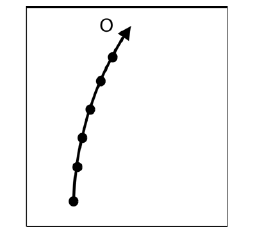
\includegraphics[scale=1]{immagini/minkowski/linea_universo}
   \caption{Linea di universo di un osservatore. I punti sono i ``battiti'' del suo orologio.}
\end{figure}

Per indagare l'universo fuori dalla sua piattaforma, l'osservatore non usa
più i regoli rigidi di Newton, bensì i segnali luminosi, scelti per la loro caratteristica 
di essere i segnali che si propagano alla velocità (limite) della luce\footnote{Inoltre, come si vedrà più avanti
nel capitolo relativo alle conferme sperimentali della relatività speciale ed ai paradossi relativistici, 
il modello di corpo rigido va in crisi in ambito relativistico.}. 
Per individuare un evento $E$ fuori dalla linea di universo dell'orologio, l'osservatore 
invia un segnale luminoso al tempo $T_1$, misurato dal suo orologio, in
modo tale che il segnale arrivi nel punto di accadimento dell'evento $E$ esat-
tamente quando $E$ accade, e poi misura il tempo di arrivo $T_2$ dell'eco riflessa.
La situazione è chiarita anche dalla figura \ref{radar1}, questa procedura è anche detta
\textbf{metodo dei segnali radar} o semplicemente ``metodo radar''.

\begin{figure}[htbp]
   \centering
   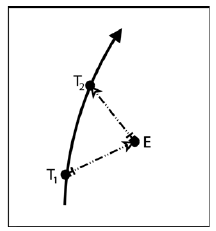
\includegraphics[scale=1]{immagini/minkowski/radar1}
   \caption{\label{radar1} Individuazione di un evento. Per convenzione indicheremo i segnali luminosi con queste particolari frecce trattopuntate.}
\end{figure}

I regoli di Newton sono stati sostituiti da ``regoli di luce'' e tutte le misure
sono ricondotte a misure di tempo eseguite con un unico orologio posto nella
piattaforma dell'osservatore locale.

\subsection{Misure di spazio, misure di tempo}
Il fatto di ricondurre tutte le misure spaziali a misure di tempo (cosa che
accade con questo ``metodo radar''), è un'ampliamento di prospettive e una
semplificazione concettuale. Possiamo portare come esempio quanto scrive
H. Bondi:
\begin{quote}
``Immaginiamo una civiltà in cui il metro sia sconosciuto e ogni distanza espressa in secondi-luce o 
millimicrosecondi-luce o in qualsiasi altra unità opportuna; i membri di questa società considererebbero
piuttosto sciocco chi chiedesse il valore della velocità della luce, essi
non la considererebbero una quantità da esprimere in metri al secondo
o chilometri al secondo, ma semplicemente come una unità, l'unità
naturale di velocità. La velocità di un oggetto verrebbe misurata paragonandola 
a quella della luce: tutte le velocità ordinarie sarebbero
espresse in termini di questo campione. [...] In altre parole accettando 
come campione di velocità [...] la velocità della luce, questa
civiltà avrebbe eliminato la necessità di costruire oltre a un campione
di tempo anche uno di lunghezza, e di usare uno scomodo numero per
esprimere la velocità della luce. In questa civiltà esisterebbe solo un
campione di tempo, i suoi componenti ci considererebbero delle persone 
che lavorano con lunghezze e tempi nel modo più complicato e
assurdo.''

(Hermann Bondi, La relatività e il senso comune, Zanichelli, pp. 36-37)
\end{quote}

Si consideri infatti:
\begin{quote}
``[...] una civiltà in cui la direzione nord-sud viene considerata sacra
ed è sempre misurata in miglia, mentre quella est-ovest viene considerata 
volgare e profana ed è sempre misurata in yarde. Se la gente
venisse abituata a vedere le cose sotto questo aspetto fin dalla prima
età, occorrerebbe una mente audace per suggerire l'esistenza di un
qualche legame tra le distanze nella direzione nord-sud e quelle nella
direzione est-ovest.''

(ibidem, p. 37)
\end{quote}

La stessa cosa accade dunque per noi: abbiamo sempre concepito spazio
e tempo come entità separate, cosicchè ci è costata fatica vederle come varie
declinazioni di un unico spaziotempo. In un'ottica unitaria di questo tipo
non c'è alcuna ragione di considerare anche un campione di lunghezza (come
ad esempio un regolo graduato): ci basta usare un campione di tempo, che
legheremo poi mediante $c$ alle quantità spaziali.

\section{Osservatori localmente inerziali}
Fin qui non vi è alcun modo di privilegiare un osservatore rispetto ad un
altro. Però possiamo constatare fisicamente che esiste una classe privilegiata
di osservatori locali, che chiameremo osservatori localmente inerziali.
Consideriamo, ad esempio, una navicella spaziale che navighi a motori spenti
in un'orbita interplanetaria. L'esperienza mostra che all'interno della navicella 
tutto avviene come previsto dalla teoria newtoniana degli osservatori
inerziali: due particelle lasciate libere o stanno ferme o si muovono di moto
rettilineo uniforme, un giroscopio messo in rotazione ha l'asse in direzione
invariabile, e così via. Ammettiamo perciò, come primo assioma, l'esistenza
di osservatori localmente inerziali (ove l'avverbio ``localmente'' si riferisce al
fatto che le osservazioni sono sempre locali, in un intorno dell'osservatore),
gli osservatori che cioè, sulla loro piattaforma, vedono le particelle libere soddisfare 
al principio di inerzia, i giroscopi in rotazione avere l'asse in direzione fissa, e così via.
Una questione interessante è comprendere l'origine degli osservatori inerziali. 
La risposta accettata oggi è che gli osservatori inerziali sono determinati 
dalla distribuzione di massa nell'universo (principio o punto di vista di
Mach\footnote{Ernst Mach (1838-1916), filosofo e fisico austriaco di grande influenza su Einstein e su
tutto il pensiero moderno.}). Una conferma di questo punto di vista viene dall'osservazione sperimentale 
la quale mostra che, rispetto a tali osservatori, il complesso delle
stelle che popolano l'universo appare fisso (e non ruotante): questo ci dice che
c'è una relazione misteriosa tra questi osservatori e la materia nell'universo.
Quindi l'origine degli osservatori localmente inerziali, detti anche osservatori
in caduta libera, starebbe in una proprietà globale dell'universo e dello spaziotempo 
che lo rappresenta. 

Gli osservatori localmente inerziali si riconoscono sperimentalmente facendo semplici 
esperienze meccaniche con particelle libere, che devono essere o ferme o muoversi di moto uniforme, con oscillatori, 
che non devono allungarsi, e con giroscopi, il cui asse non deve cambiare direzione.

Introdotti gli osservatori localmente inerziali, si studia poi il loro assemblamento 
(ossia come essi sono collegati). Consideriamo due osservatori inerziali
$O$ e $O'$ . Mediante il metodo dei segnali radar ognuno dei due può decidere se
l'altro è in quiete o in moto rispetto a lui. La condizione di quiete è espressa
dall'invarianza dell'intervallo di tempo T tra emissione e ricezione del segnale
radar, scambiato tra i due osservatori (come mostra la figura \ref{osservatori_radar} qui sotto).

\begin{figure}[htbp]\label{osservatori_radar}
   \centering
   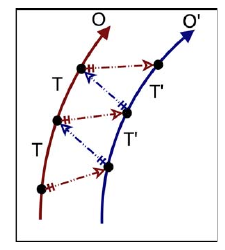
\includegraphics[scale=1]{immagini/minkowski/osservatori_radar}
   \caption{Scambio reciproco di segnali luminosi tra osservatori.}
\end{figure}

La proprietà vale tanto per il primo quanto per il secondo osservatore. Si
constata inoltre che se gli osservatori sono “suffientemente” vicini (situazione 
corrispondente a periodi $T$ e $T'$ ``sufficientemente'' piccoli) è possibile
calibrare gli orologi dei due osservatori in modo tale che $T$ = $T'$. Questo
processo di calibrazione prende il nome di sincronizzazione degli orologi
inerziali in quiete relativa.
Riepilogando: l'esperienza mostra che esistono osservatori localmente
inerziali in quiete relativa che possono essere sincronizzati tra loro. Rimane
aperto il problema dell'estensione di questo processo. Il processo di sincronizzazione 
di osservatori inerziali in grande è in generale impossibile. Tale
processo funziona solo per osservatori ``sufficientemente'' vicini: quando si
superano certe distanze e certi intervalli di tempo, cominciano a comparire 
delle discrepanze e si manifesta l'impossibilità di sincronizzare in grande
osservatori localmente inerziali nel modo prima descritto.

\section{Lo spaziotempo di Minkowski}
Si chiama spaziotempo di Minkowski uno spaziotempo ideale in cui si ammette 
che il processo di sincronizzazione prima descritto valga in grande. Lo
spaziotempo di Minkowski è quindi il modello di spaziotempo dove esistono
osservatori globalmente inerziali, costituiti da una rete di osservatori localmente inerziali 
in quiete relativa, sempre nel senso dello scambio di segnali
luminosi, e sincronizzati tra loro.

Lo spaziotempo di Minkowski è quindi un'approssimazione dello spazio-tempo fisico 
che può essere paragonata all'approssimazione che lo spazio tan-
gente fornisce di una superficie curva in un suo punto.

Nello spazio tangente possiamo parlare di rette e di rette parallele, mentre
sulla superficie possiamo solo parlare di geodetiche.Infatti le rette rimangono parallele 
in ogni punto dello spazio tangente, mentre le corrispondenti
geodetiche divergono sulla superficie a causa della curvatura della superficie.

Le rette e le geodetiche devono essere confrontate con le linee di universo degli
osservatori localmente inerziali nello spaziotempo. Rette parallele corrispon\-dono
ad osservatori inerziali in quiete relativa. Nello spaziotempo di Minkowski 
(corrispondente allo spazio tangente) queste linee di universo rimangono
sempre parallele, nello spaziotempo fisico invece no, a significare che dopo
un po' il processo di sincronizzazione diventa impossibile. L'impossibilità di
definire mediante il processo di sincronizzazione un osservatore globalmente
inerziale è quindi una misura della ``curvatura'' dello spaziotempo.

Nel modello di Minkowski, invece, si assume che esistano osservatori globalmente inerziali; 
ciò corrisponde a sviluppare una teoria dello spaziotempo
piatto. Questa teoria è la Relatività Ristretta. Essa è una buona approssimazione 
del mondo fisico in una scala di misure sulla quale si possono
trascurare gli effetti delle forze gravitazionali. La fisica nello spazio di Minkowski 
è, in sostanza, una fisica in assenza di gravità: in questa situazione è
possibile il processo di sincronizzazione prima descritto.
Su scale più grandi, dove non è possibile trascurare l'effetto delle forze
gravitazionali prodotte dalle grandi masse distribuite nell'universo, le forze
gravitazionali si manifestano come cause distorcenti il processo di sincronizzazione 
(influenti sul moto dei segnali luminosi), cosicchè l'approssimazione
dello spaziotempo di Minkowski non risulta più valida e bisogna passare all Relatività Generale. 
In sostanza, la Relatività Generale è la geometria dello spazio tempo quando si 
tiene conto dell'impossibilità della sincronizzazione in grande di osservatori
localmente inerziali.

Riassumendo:
\begin{itemize}
 \item il concetto di osservatore ha validità locale ed esistono degli osservatori
privilegiati detti localmente inerziali;
 \item in una prima approssimazione, è possibile parlare di osservatori localmente 
inerziali in quiete relativa e sincronizzare i rispettivi orologi in 
modo che misurino lo stesso periodo nei segnali scambiati;
 \item questo processo di sincronizzazione è solamente locale. Una buona
approssimazione dello spaziotempo reale è fornita dal modello ideale
in cui si ammette che la nozione di quiete relativa e il processo di
sincronizzazione abbiano validità globale. Questa proprietà definisce lo
spaziotempo di Minkowski.

\end{itemize}

\subsection{Il cono luce}

Immaginiamo di considerare nello spaziotempo di Newton due osservatori
inerziali in moto relativo l'uno rispetto all'altro, muniti dello stesso dispo-
sitivo per lanciare palline (pensate come punti materiali). Supponiamo che
a un certo istante i due osservatori si trovino nello stesso luogo (chiamiamo
questo evento $O$), e che lancino insieme le due palline. Le figure \ref{palline_raggi}
mostrano che cosa accade e che cosa accadrebbe se invece di lanciare pal\-line 
nello spazio newtoniano lanciassero segnali luminosi secondo la visione
di Einstein.

\begin{figure}[htbp]\label{palline_raggi}
   \centering
   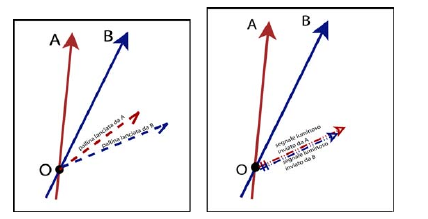
\includegraphics[scale=1]{immagini/minkowski/palline_raggi}
   \caption{A sinistra: palline lanciate da osservatori inerziali in moto rela-
tivo in un universo newtoniano. A destra: segnali luminosi inviati dagli stessi
osservatori inerziali in moto relativo in un universo einsteiniano.}
\end{figure}

Nel caso newtoniano, la velocità degli oggetti lanciati dipende dalla velocità della sorgente, 
e quindi le linee di universo delle palline lanciate da $A$ e $B$ nell'evento $O$, in generale, differiscono. Dunque non vi 
è alcuna linea di universo privilegiata rispetto alle altre.

Viceversa, nel caso di Einstein, il postulato riguardo all'invarianza di $c$
richiede che la velocità della luce non dipenda dalla velocità della sorgente.

Quindi due raggi luminosi, inviati in una data direzione da due sorgenti
che viaggiano con velocità diverse, viaggeranno comunque con la medesima
velocità. Il che equivale a dire che per ogni direzione spaziale vi è un'unica e
ben determinata linea di universo del segnale luminoso. 
L'insieme di queste linee di universo forma il ``cono luce'' associato all'evento considerato (v. figura
\ref{coni_luce}). 

\begin{figure}[htbp]
   \centering
   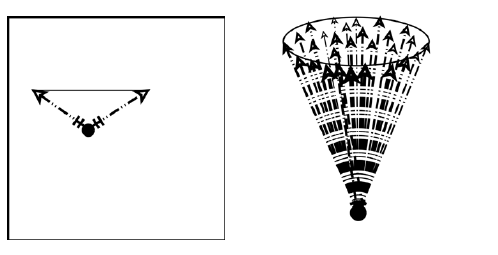
\includegraphics[scale=1]{immagini/minkowski/coni_luce}
   \caption{\label{coni_luce}Coni luce in universi (rispettivamente) bidimensionale e tridimen-
sionale. In un universo bidimensionale i possibili raggi inviati sono solamente due.}
\end{figure}

Nel caso di un universo bidimensionale, essendoci solo due direzioni
possibili per il raggio luminoso, il cono luce degenera a una sorta di triangolo.

\subsection{$c$ come velocità limite}

Lo spazio di Minkowski è utile per dare un significato geometrico alla relatività speciale.
Per comodità grafiche consideriamo solo una coordinata spaziale e una temporale. Sull'asse delle ascisse rappresentiamo $x$ 
e sull'asse delle ordinate, che chiamiamo $w$ il tempo moltiplicato per $c$, che lo rende uno spazio.
La bisettrice dei quadranti ha equazione:
\begin{equation}
 x = w = ct
\end{equation}
ed è la linea di universo della luce, essa rappresenta il cammino di un raggio luminoso.

Invece la linea di universo di un qualsiasi corpo dotato di massa che si muove con velocità $v$ dovrà avere
coefficiente angolare dato da:
\begin{equation}
\frac{\ud w}{\ud x}=\frac{\ud(ct)}{\ud x}=c\frac{1}{\frac{\ud x}{\ud t}}=\frac{c}{v}>1 
\end{equation}

Quindi la traiettoria di ogni punto massivo nel piano di Minkowski deve avere tangente in ogni 
punto maggiore di uno, altrimenti andrebbe più veloce della luce.

\subsection{Osservatori nello spaziotempo di Minkowski}

Creiamo un nuovo sistema di riferimento inerziale.
Partiamo dalle trasformazioni di Lorentz:
\begin{equation}
\left\{\begin{array}{l}
x'=\frac{x-ut}{\sqrt{1-\beta^2}}\\
t'=\frac{t-\frac{\beta}{c}x}{\sqrt{1-\beta^2}}\\
\end{array}\right. 
\end{equation}

Se moltiplichiamo e dividiamo per $c$ ogni qual volta che abbiamo una velocità, ricordando che
$w = ct$ e $\beta = \frac{u}{c}$, abbiamo che:
\begin{equation}\label{x_w_to_xp_wp}
\left\{\begin{array}{l}
x'=\frac{x-\beta w}{\sqrt{1-\beta^2}}\\
w'=\frac{w-\beta x}{\sqrt{1-\beta^2}}\\
\end{array}\right. 
\end{equation}

Se vogliamo disegnare il nuovo sistema di riferimento $(x', w')$ 
dobbiamo ricavarne le equazioni rispetto al sistema di riferimento $(x, w)$
quindi:
\begin{equation}
\left\{\begin{array}{l}
\text{asse} \; x': w'=0 \\
w'=\frac{w-\beta x}{\sqrt{1-\beta^2}}\\
\end{array}\right. 
\qquad
\left\{\begin{array}{l}
x'=\frac{x-\beta w}{\sqrt{1-\beta^2}}\\
\text{asse} \; w': x'=0
\end{array}\right.  
\end{equation}
Da cui si ricavano le equazioni degli assi $x'$, $w'$:
\begin{equation}
 \left\{\begin{aligned}
  &\text{asse} \; x': &w &=\beta x \\
  &\text{asse} \; w': &w &= \frac{1}{\beta } x  \\
 \end{aligned}\right.  
\end{equation}

Più $\beta$ tende a $1$ e più i due assi del nuovo sistema di riferimento tendono alla bisettrice del primo--terzo quadrante.

I sistemi che abbiamo costruito sono rappresentati nella figura \ref{Mink2}.
\begin{figure}
   \centering
   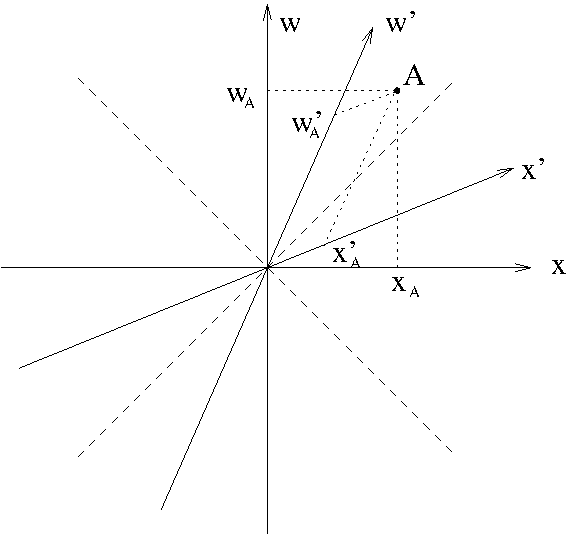
\includegraphics[scale=1]{immagini/minkowski/Mink2}
   \caption{\label{Mink2} ``Costruzione'' di un osservatore nello spaziotempo di Minkowski.}
\end{figure}


\subsubsection{Curve di calibrazione\index{curve! di calibrazione}}

Come rappresentato in figura \ref{Mink2} posso rappresentare un osservatore con un sistema di riferimento cartesiano.
L'osservatore che riteniamo fermo è rappresentato dagli assi $x \hat O w$, quello in moto dagli assi $x' \hat O' w$. Indichiamo 
le coordinate rispetto al sistema $x \hat O w$ con $(x,w)$ e quelle rispetto al sistema $x' \hat O' w$ con $(x',w')$.

Per trasportare una misura da un sistema all'altro è necessario applicare le trasformazioni di Lorentz, per facilitare questo
processo si disegnano le ``curve di calibrazione''.  Esse sono date dalle seguenti equazioni:
\begin{equation}
\left\{\begin{array}{l}
x^2 - w^2 =  1\\
x^2 - w^2 = -1\end{array}\right. 
\end{equation}

\begin{figure}[htbp]
   \centering
   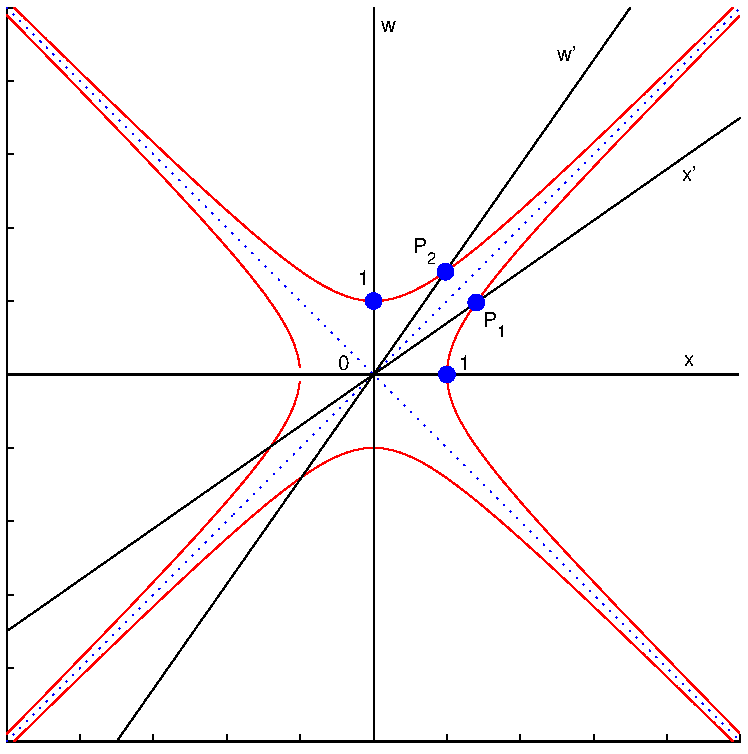
\includegraphics[scale=0.7]{immagini/minkowski/Minkowski_calibrazione}
   \caption{\label{Minkowski_calibrazione}Curve di calibrazione nello spaziotempo di Minkowski.}
\end{figure}


Queste curve, rappresentate nella figura \ref{Minkowski_calibrazione}, ci permettono di trasportare il segmento 
unitario nella direzione spaziale o temporale del sistema $x \hat O w$ a quello del sistema  $x' \hat O' w$.

Infatti il punto $P: (1, 0)$ ovvero l'unità di lunghezza nel sistema $x \hat O w$ viene trasportata nel punto $P'$
le cui coordinate sono date da:
\begin{equation}
\left\{\begin{array}{l}
x^2-w^2=1\\
\text{asse} \; x': w'=0 \rightarrow w =\beta x \\
\end{array}\right. 
\end{equation}

da cui si ricavano le coordinate di $P'$ rispetto al sistema $x \hat O w$, ovvero\footnote{Ricordiamo che $0 \leq \beta < 1 $, 
quindi le relazioni sono ben definite}:
\begin{equation}
P' \left\{\begin{aligned} 
x &= \frac{1}{\sqrt{1-\beta^2}}\\
w &= \frac{\beta}{\sqrt{1-\beta^2}}
\end{aligned}\right. 
\end{equation}
Il punto $P'$ corrisponde a $(1', 0')$, ossia
all'unità di lunghezza nel sistema $x' \hat O' w$, infatti usando \ref{x_w_to_xp_wp}:
\begin{equation}
 \left\{
 \begin{aligned}
 x' &= \dfrac{\dfrac{1}{\sqrt{1-\beta^2}}-\beta w}{\sqrt{1-\beta^2}} = \dfrac{\dfrac{1}{\sqrt{1-\beta^2}}-\dfrac{\beta^2}{\sqrt{1-\beta^2}}}{\sqrt{1-\beta^2}} = 1 \\
 w' &= \dfrac{\beta}{\sqrt{1-\beta^2}} - \beta \dfrac{1}{\sqrt{1-\beta^2}} = 0
 \end{aligned}
 \right. 
\end{equation}

Da questi diagrammi è possibile ottenere in modo diverso gli effetti di dilatazione dei tempi e di contrazione delle lunghezze.

\subsubsection{Le trasformazioni di Lorentz come rotazioni iperboliche\index{le trasformazioni di Lorentz! come rotazioni iperboliche}}


\subsection{La struttura di causalità dello spaziotempo}
La velocità della luce è invariante, ma abbiamo anche postulato che sia una
velocità limite, ovvero che non esistano sistemi o segnali fisici che possano
oltrepassare tale velocità. Questa proprietà ci è utile per stabilire la relazione
tra osservatori inerziali e coni luce.

La questione che ci poniamo è: come sono disposte le linee di universo
degli osservatori inerziali rispetto ai coni luce? La risposta è che le linee
di universo di tali osservatori devono necessariamente cadere all'interno del
cono, poichè essendo $c$ velocità limite, un segnale che viaggiasse al di fuori
dal cono avrebbe pendenza minore, e dunque una velocità maggiore di $c$.

\begin{figure}[htbp]
   \centering
   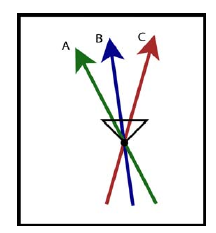
\includegraphics[scale=0.7]{immagini/minkowski/osservatori_coni_luce2}
   \caption{\label{osservatori_coni_luce2} Possibili linee di universo per osservatori massivi.}
\end{figure}

\begin{figure}[htbp]
   \centering
   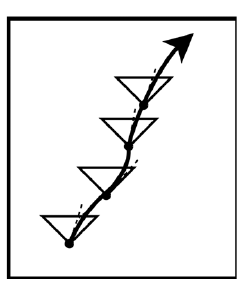
\includegraphics[scale=0.7]{immagini/minkowski/osservatori_coni_luce3}
   \caption{Da ogni punto dello spazio tempo possiamo fare partire un cono luce.}
\end{figure}


Il carattere di velocità limite di $c$ implica quindi che le linee di universo degli 
ossevatori inerziali siano contenute nel cono luce. Queste linee di universo
sono dette linee del genere tempo. Da questa osservazione segue subito la divisione (relativamente a un
evento prefissato $O$) dello spaziotempo $M$ in tre regioni distinte (v. figura
\ref{struttura_causale}):

\begin{figure}[htbp]
   \centering
   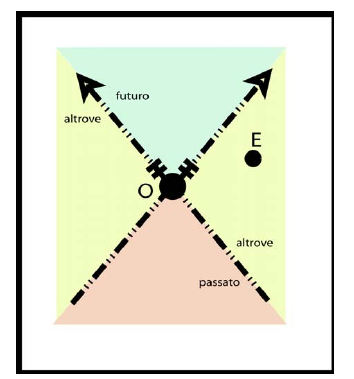
\includegraphics[scale=0.7]{immagini/minkowski/struttura_causale}
   \caption{\label{struttura_causale} La ``struttura causale'' dello spaziotempo.}
\end{figure}

\begin{itemize}
 \item futuro: è la falda del cono che contiene le linee del genere tempo, nel
senso dell'orientamento delle linee di universo degli osservatori;
 \item passato: l'altra falda del cono;
 \item altrove: tutta la parte rimanente dello spaziotempo
\end{itemize}

Questa distinzione ha un significato fisico profondo: distingue gli eventi
che possono essere influenzati da $O$ (futuro) dagli eventi che possono aver
influenzato $O$ (passato) e da quelli che non possono essere messi in relazione
causale con $O$ (altrove). Vedremo infatti che, se possiamo dare un ordinamento 
temporale per gli eventi del futuro e del passato (possiamo dire quindi
univocamente se $E$ avviene prima o dopo $O$, nel senso che tutti gli osservatori
concordano su ciò), a eventi situati nell'altrove non riusciremo ad attribuire
una consequenzialità temporale: ci saranno osservatori che li diranno simultanei a O, 
altri che li vedranno accadere prima di $O$, altri ancora che li
vedranno accadere dopo $O$.

L'assioma riguardo all'invarianza di $c$ si traduce geometricamente in modo molto
particolare, esso infatti è la prima struttura geometrica dello spaziotempo di Minkowski 
(indicato con $M$) , detta ``struttura di causalità'', poichè
essa regola il segno del divario temporale tra gli eventi, e quindi stabilisce
l'ordinamento temporale che è alla base del principio di causa-effetto. Se
vogliamo affermare, infatti, che un evento $A$ è causa di un evento $B$, deve
quantomeno sussistere il fatto che $A$ accada prima di $B$. Per confronto con
la cinematica newtoniana, vediamo che cosa implica l'assioma dell'invarianza
di $c$ nella geometria di $M$.

\subsection{Coordinate di un evento}
Stabilita la traduzione geometrica degli assiomi, cominciamo a vedere come
ogni osservatore inerziale individua, con le sue coordinate relative, ogni evento;
in linguaggio geometrico, costruiamo il sistema di coordinate globali su $M$
associato ad un dato osservatore inerziale. Non ci sono più regoli, e quindi il
meccanismo è interamente basato sui segnali luminosi.

Dato un osservatore $A$, innanzitutto introduciamo le coordinate radar
$(T_1 , T_2)$ dell'evento $E$, definite facendo riferimento ancora alla figura
\ref{osservatori_radar} come segue:
\begin{itemize}
 \item $T_1$: è il tempo di emissione (rispetto all'orologio dell'osservatore A) del
segnale luminoso emesso da $A$ che giunge in $E$;
 \item $T_2$: è il tempo di ricezione del segnale riflesso (sempre nel giudizio di $A$).

\end{itemize}

In linguaggio geometrico, le coordinate radar non sono nient'altro che le
intercette del cono luce di vertice $E$ con la linea di universo dell'osservatore
$A$.
Si passa poi alle coordinate spaziotemporali $(x, t)$ dell'evento mediante le
seguenti definizioni:
\begin{equation}
 \begin{aligned}{ll}
  ct &= \dfrac{1}{2} c(T_2 + T_1 ) \\
  x &= \dfrac{1}{2} c(T_2 - T_1 )
 \end{aligned}
\end{equation}

Sostanzialmente stiamo definendo il tempo dell'evento $E$ come media dei
due tempi (tempo di emissione e tempo di ricezione), e come spazio lo spazio
percorso dal raggio luminoso nella semisomma dei tempi, ossia nella metà
del periodo emissione-ricezione.

Occorre puntare l'attenzione sul fatto che tali definizioni sono le uniche
definizioni plausibili con le informazioni in nostro possesso (solo $T_1$ , $T_2$ e
$c$), ipotizzando tacitamente che lo spazio sia isotropo, ossia che la velocità
della luce non cambi tra andata e ritorno. Non abbiamo altra scelta che
prendere come tempo il tempo medio di riflessione: secondo il punto di vista
dell'osservatore $A$, la luce, per giungere ad $E$, deve impiegare lo stesso tempo
che impiega per tornare indietro.

\subsection{L'effetto Doppler longitudinale}
Veniamo ora al problema centrale della nostra analisi: quello del confronto tra diversi 
osservatori inerziali in moto relativo, passo indispensabile per la scoperta delle 
caratteristiche comuni ai vari osservatori e della geometria dello spaziotempo.

Il nucleo della questione è il confronto tra gli orologi dei due osservatori
in moto. Questo confronto è fatto misurando il periodo di emissione e il
periodo di ricezione (ognuno nel giudizio del corrispondente osservatore) in un
processo di scambio di segnali luminosi periodici - essendo i segnali luminosi
l'unico mezzo che gli osservatori hanno a disposizione per confrontarsi.

Sia $T_e$ il periodo di emissione nel giudizio di $A$, e sia $T_r$ il periodo di
ricezione valutato da $B$. Se $B$ si allontana da $A$ con velocità 
relativa\footnote{Si presti attenzione a questo particolare: se avessimo a che fare con l'effetto Doppler acustico
(cioè il fenomeno per cui un suono cambia frequenza all'avvicinarsi/allontanarsi di sorgente o osservatore) 
non potremmo considerare solo la velocità relativa tra sorgente e osservatore.
Avendo, infatti, l'onda sonora bisogno di un mezzo (l'aria) per propagarsi, è necessario
considerare le velocità rispetto all'aria sia della sorgente, sia dell'osservatore. Nella nostra
analisi radar, invece, tutto questo non è necessario: l'onda elettromagnetica non ha bisogno 
di alcun mezzo per propagarsi. Quindi l'effetto Doppler relativistico è molto più
semplice da trattare rispetto a quello ``classico'' (acustico)} $v$,
deve necessariamente essere che $T_r > T_e$ , poichè il secondo segnale ha dovuto
percorrere una distanza maggiore per raggiungere $B$. In generale, poniamo
\begin{equation}
T_r = k(v) \cdot Te  
\end{equation}
con $k(v) > 0$ funzione della velocità relativa $v$ tra i due
osservatori. Avremo che $k > 1$ se i due osservatori si allontanano, $k = 1$ se
i due osservatori sono in quiete relativa, $0 < k < 1$ se i due osservatori si
avvicinano. Il fattore $k$, termine centrale nel nostro studio (da cui, appunto,
il nome di $k$-calcolo), viene detto ``fattore 
Doppler\footnote{Christian Johann Doppler (1803-1853), fisico austriaco.}
 longitudinale'', l'aggettivo ``longitudinale'' sta ad indicare che i segnali luminosi sono emessi
nella direzione del moto relativo dei due osservatori.

Disponiamo solamente di due informazioni:
\begin{enumerate}
 \item $B$ si muove di moto relativo con velocità $v$ rispetto ad $A$;
 \item il Principio di Relatività;
\end{enumerate}
Queste informazioni sono sufficienti per risolvere il problema. 
Supponiamo infatti di avere due osservatori in moto relativo $B$ ed 
$A$, come descritto dalla figura \ref{doppler}. Secondo l'osservatore
$A$, $B$ si muove secondo la legge:
\begin{equation}\label{moto_relativo}
x=vt 
\end{equation}
con $(x, t)$ coordinate di $B$ nel giudizio di $A$.

\begin{figure}[htbp]
   \centering
   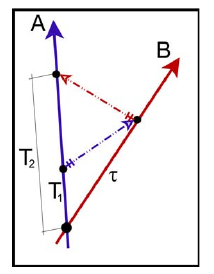
\includegraphics[scale=1]{immagini/minkowski/doppler}
   \caption{\label{doppler} Doppio scambio Doppler. Gli istanti temporali 
sono interpretati come periodi di tempo del doppio scambio Doppler
tra $A$ e $B$: $T_1$ è il periodo di emissione da parte di $A$ di un segnale periodico
ricevuto da $B$ con un periodo di ricezione $\tau$; $T_2$ è il periodo di ricezione da
parte di $A$ di un segnale periodico emesso da $B$ con un periodo $\tau$.}
\end{figure}

Il nodo centrale è interpretare la figura \ref{doppler} dal punto di vista dell'effetto
Doppler, convenendo che $A$ e $B$ si scambino un primo segnale (una sorta di
``azzeramento'' degli orologi) in $O$. In questo modo convertiamo le coordinate
radar in periodi.

Ciò che succede è che $A$ e $B$ sincronizzano gli orologi quando si incontrano;
dopo un tempo $T_1$ (nel giudizio di $A$), $A$ lancia un segnale luminoso che arriva
al tempo $\tau$ (nel giudizio di $B$) all'osservatore $B$, il quale lo rispedisce subito
indietro. Il segnale ritorna al tempo $T_2$, nel giudizio di $A$, all'osservatore $A$.
Il diagramma \ref{doppler} del moto relativo serve a localizzare $B$ nel giudizio di
$A$. Infatti ($T_1$ , $T_2$) sono esattamente le coordinate radar di $B$, in particolare
sono le coordinate dell'evento $E$ ``ricezione del segnale da parte di $B$'', rispetto ad $A$. 
Quindi le equazioni:
\begin{equation}
 \begin{array}{ll}
  ct &= \frac{1}{2} c(T_2 + T_1) \\
  x &= \frac{1}{2} c(T_2 - T_1)
 \end{array}
\end{equation}
forniscono la posizione e il tempo di $B$ nel giudizio di $A$. 
Unendo questo risultato all'informazione \ref{moto_relativo}, possiamo scrivere che
\begin{equation}\label{doppler1}
 \dfrac{v}{c} = \dfrac{x}{ct} =\dfrac{T_2 - T_1}{T_2 + T_1} 
\end{equation}

Ora colleghiamo le coordinate radar con il fattore Doppler, osservando
che $\tau$, nel grafico dello scambio Doppler, è esattamente il periodo di ricezione
da parte di $B$ di un treno d'onde emesso da $A$ con periodo $T_1$ abbiamo:
\begin{equation}\label{doppler2}
\tau = k_{AB} (v) \cdot T_1
\end{equation}
con $k_{AB} (v)$ fattore Doppler longitudinale quando $A$ emette e $B$ riceve. Allo
stesso modo, posso interpretare $T_2$ come periodo di ricezione da parte di $A$ di
un treno d'onde emesso da $B$ con periodo $\tau$, ne deduciamo che:
\begin{equation}\label{doppler3}
T_2 = k_{BA} (v) \cdot \tau
\end{equation}
con $k_{BA} (v)$ fattore Doppler longitudinale quando $B$ emette e $A$ riceve.
Ma il Principio di Relatività impone che ci sia completa simmetria tra
$A$ e $B$, ovvero che\footnote{Il simbolo $:=$ significa ``per definizione''}:
\begin{equation}
k_{BA} (v) = k_{AB} (v) := k(v).
\end{equation}
Se non fosse così infatti, avremmo modo di scegliere un osservatore privilegiato, ad esempio, 
l'osservatore che ha il minor $k$ quando emette i segnali luminosi).
Ne deduciamo che devono valere le seguenti tre equazioni \ref{doppler1}, \ref{doppler2},
\ref{doppler3} si ricava quindi che:
\[
 \dfrac{v}{c} = \dfrac{k - k^{-1}}{k + k^{-1}} = \dfrac{k^2 -1}{k^2 +1}
\]
ovvero: $vk^2 + v = ck^2 - c$, da cui
\begin{equation}
k = \sqrt{\dfrac{c+v}{c-v}} 
\end{equation}
Dunque, se $B$ si allontana da A, abbiamo che $v > 0$, ovvero $k > 1$. Se $A$
e $B$ sono in quiete relativa, abbiamo che $v = 0$, ovvero $k = 1$. Se infine $B$ si
avvicina ad $A$, abbiamo che $v < 0, k < 1$.


\chapter{Conferme sperimentali della relatività speciale}
\minitoc

\section{Il decadimento dei mesoni}

I raggi cosmici, quando arrivono al bordo superiore dell'atmosfera, ad una quota di 
circa $h = 20\;km$ rispetto al livello del mare, producono nell'urto con
l'atmosfera delle particelle instabili, dette mesoni (e solitamente indicati con
la lettera greca $\mu$), che viaggiano nell'atmosfera con velocità $v \approx 0.99c$ 
(pari alla velocità dei raggi cosmici che li producono). 

\begin{figure}[htbp]
   \centering
   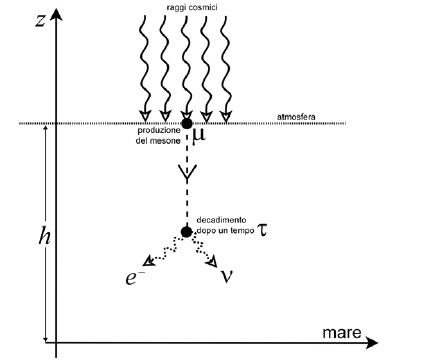
\includegraphics[scale=1]{immagini/conferme_relspec/produzione_mu}
   \caption{\label{produzione_mu}Produzione e decadimento dei mesoni $\mu$. Il mesone viene prodotto 
dall'urto dei raggi cosmici con l'atmosfera, a un'altezza $h$. Dopo un
tempo $\tau$ esso decade in un elettrone e un neutrino.}
\end{figure}

Queste particelle instabili hanno una vita media $\tau$ che è legata alla legge di decadimento
\begin{equation}
N(t) = N_0 e^{-\lambda t}
\end{equation}

con $\tau = \dfrac{1}{\lambda}$. Nell'equazione, $N(t)$ è il numero di particelle a un
istante $t$, $N_0$ è il numero di particelle iniziali.

La vita media $\tau$ può essere misurata in laboratorio (quando i mesoni
sono a riposo), valutando la porzione di popolazione iniziale che dopo un
dato tempo $t$ non è decaduta in elettroni e neutrini. 

Abbiamo quindi tutti i dati del problema: altezza $h$, velocità $v$ e vita media $\tau$.

Secondo la fisica newtoniana, lo spazio percorso dal mesone $\mu$ tra la
nascita e la morte è

\begin{equation}
s = vt 
\end{equation}

Se si inseriscono i dati, si trova che $vt < h$, cioè che $s < h$, e quindi non
dovrebbe essere possibile rilevare mesoni di origine cosmica al livello del mare.
Al contrario, tali mesoni sono rilevati.

Vogliamo quindi dare una spiegazione a questo fenomeno, usando in modo duale sia 
la dilatazione dei tempi, sia la contrazione delle lunghezze.

\subsection{Punto di vista della terra}
Dal punto di vista della terra, la spiegazione si basa sulla dilatazione dei
tempi: la vita media $\tau$ è un tempo misurato da un ``orologio interno'' del mesone.

Possiamo schematizzare la faccenda nel diagramma di figura \ref{diagramma_mu}.

\begin{figure}[htbp]
   \centering
   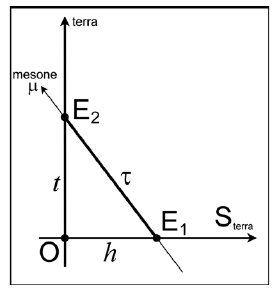
\includegraphics[scale=1]{immagini/conferme_relspec/diagramma_mu}
   \caption{\label{diagramma_mu}Diagramma spaziotemporale della vita del mesone. L'evento
$E_1$ è la produzione del mesone, l'evento $E_2$ è il suo rilevamento a terra.}
\end{figure}

Il punto fondamentale è prestare attenzione, al fine di non confondere le
misure di spazio e di tempo fatte dall'osservatore terrestre con quelle fatte dal
mesone, poichè entrambe le misure hanno valore relativo. Dato che l'esperienza 
ci dice che riusciamo a trovare mesoni al livello del mare, ribatteziamo
$\tau$ il tempo (minimo) tra la produzione e il rilevamento del mesone nel giu-
dizio del mesone. Sia invece $t$ il tempo tra gli stessi eventi nel giudizio del
laboratorio terrestre. I due eventi $E_1$ (produzione del mesone) ed $E_2$ (rileva-
mento del mesone) avvengono sulla linea di universo del mesone, quindi $\tau$ è
il tempo proprio. Per la dilatazione dei tempi abbiamo che
\[ t = \gamma (v) \cdot \tau\]

Questa è stata una delle prime verifiche sperimentali della validità della Relatività
Ristretta.

La legge di moto rispetto all'osservatore terrestre\footnote{Prestiamo attenzione: 
è vero che le leggi di moto devono avere la stessa forma nel
giudizio del mesone e in quello della terra, ma dobbiamo stare attenti che in ciascuna di 
esse tutte le grandezze devono essere misurate dallo stesso osservatore. La disomogeneità
delle misure porta inevitabilmente all'invalidità delle equazioni.}
è
\[ h = vt \]
e quindi la legge corretta è:
\[ h = (\gamma (v) \cdot v) \cdot \tau \]
che è compatibile con i dati sperimentali.

Il fenomeno si spiega dunque, rispetto all'osservatore terrestre, con la
dilatazione dei tempi: sbagliavamo nel ritenere $\tau$ il tempo di vita del mesone
nel nostro giudizio; lo era nel giudizio del mesone.

\subsection{Punto di vista del mesone}
Dal punto di vista del mesone, il tempo trascorso tra gli eventi $E_1$ (produzione, 
cioè ``nascita'' del mesone) ed $E_2$ (rilevamento del mesone al livello del
mare) è proprio $\tau$, e la velocità con cui la terra precipita addosso al mesone è
sempre $v$. Dunque abbiamo ancora il paradosso che, sulla carta, dovremmo
avere:
\[ v\tau < h \]
quando invece accade il contrario. Qui non possiamo più far valere la dilatazione 
dei tempi: il tempo $\tau$ è il tempo proprio, non c'è scampo.

Il paradosso è ancora dovuto al fatto che nella legge $v\tau < h$ stiamo impiegando 
grandezze eterogenee: $\tau$ è infatti misurato dal mesone, $h$ è misurato
dalla terra. Il paradosso nasce quindi dal mischiare nella stessa equazione
del moto uniforme grandezze misurate da osservatori diversi. Se ci poniamo nel punto di vista
del mesone, dobbiamo usare il tempo $\tau$, ma anche la distanza $d$ che il
mesone attribuisce alla terra al momento della sua nascita (anche le lunghezze
sono infatti relative). La situazione è riassunta nel diagramma di figura \ref{diagramma_mu2}.

Per determinare le distanze, dobbiamo considerare l'evento $E_3$ che si trova sulla linea
di universo della terra e che è simultaneo ad $E_1$ nel giudizio del mesone.
\begin{figure}[htbp]
   \centering
   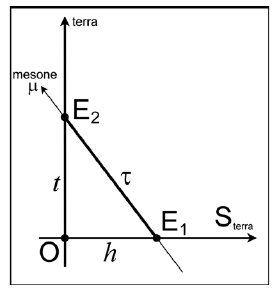
\includegraphics[scale=1]{immagini/conferme_relspec/diagramma_mu}
   \caption{\label{diagramma_mu}Diagramma spaziotemporale modificato aggiungendo il punto
di vista del mesone. In particolare, quando il mesone viene prodotto ($E_1$), nel
giudizio del mesone la terra si trova in $E_3$ . Viceversa, nel giudizio della terra,
essa si trova in $E_4$ . Quindi $k$ è la distanza tra punto di produzione e terra,
nel giudizio del mesone; $h$ è la stessa distanza nel giudizio terrestre. $\theta$ è il
parametro di rapidità.}
\end{figure}

Sia inoltre $E_4$ l'evento che avviene sulla terra contemporaneamente ad $E_1$ nel
giudizio dell'osservatore terrestre. Dal triangolo $E_1$, $E_3$, $E_4$, ricaviamo che
\[ h = d cosh \theta = \gamma(v) \cdot d \]
fatto che traduce la contrazione delle lunghezze. Quindi, nel giudizio del
mesone, la terra si trovava inizialmente a una distanza $d < h$ contratta del
fattore $cosh \theta = \gamma(v)$ rispetto alla distanza valutata dalla terra. La legge di
moto va dunque riscritta come
$d = v\tau$,
formulazione che è compatibile con i dati sperimentali.

Dunque, l'esperimento del mesone, dal punto di vista del mesone, è spiegato 
in maniera simmetrica, dalla contrazione delle lunghezze. Dilatazione
dei tempi e contrazione delle lunghezze sono perciò fenomeni duali che non
possono sussistere separatamente: l'uno implica l'altro. 

Dal punto di vista della geometria dello spaziotempo di
Minkowski, questa dualità è legata alla peculiarità delle rotazioni iperboliche
per cui, se ruota l'asse dei tempi di un osservatore, deve contemporaneamente
ruotare anche la piattaforma spaziale, in modo simmetrico rispetto al cono
luce, così da rispettare una condizione di ``perpendicolarità'' (ortogonalità) 
che ``graficamente'' è diversa dal caso euclideo.

\section{Il paradosso dei gemelli}

Consideriamo tre osservatori inerziali $A$, $B$, $C$ tali che $B$ e $C$ si muovano
rispetto ad $A$ con la stessa velocità $v$ ma da parti opposte. La situazione è
quella rappresentata in figura \ref{gemelli1}.

\begin{figure}[htbp]
   \centering
   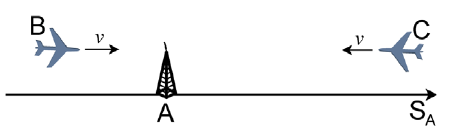
\includegraphics[scale=1]{immagini/conferme_relspec/gemelli1}
   \caption{\label{gemelli1}Situazione del paradosso dei gemelli. $B$ e $C$ si avvicinano con
velocità $v$ ad $A$; $C$ è più lontano da $A$ rispetto a $B$ (nel giudizio di $A$).}
\end{figure}

Possiamo pensare che $A$ sia la torre di controllo di un aeroporto, e che
$B$ e $C$ siano due aerei in avvicinamento. Supponiamo che, nel giudizio di $A$,
inizialmente $C$ sia molto più lontano.

\begin{figure}[htbp]
   \centering
   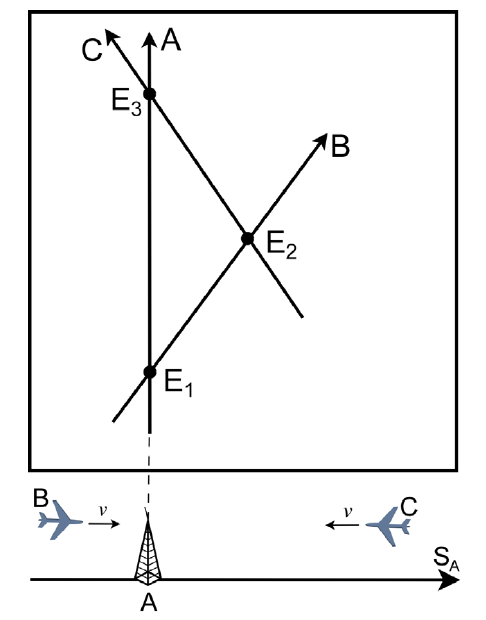
\includegraphics[scale=1]{immagini/conferme_relspec/gemelli2}
   \caption{\label{gemelli2}Situazione del paradosso dei gemelli. $B$ e $C$ si avvicinano con
velocità $v$ ad $A$; $C$ è più lontano da $A$ rispetto a $B$ (nel giudizio di $A$).}
\end{figure}

Disegnamo il diagramma spaziotemporale  e consideriamo i seguenti eventi. 
$B$ si sta avvicinando da sinistra ad $A$, sino a quando lo
incontra.
\begin{itemize}
 \item $E_1$: al tempo $t_A(E_1) = 0$ (misurato da $A$) $B$ passa per $A$, e concorda
di tarare il suo orologio in modo tale da segnare anch'esso $t_B(E_1) = 0$ (sincronizzazione degli orologi di A e B).
\end{itemize}

Poi $B$ si allontana da $A$, viaggiando verso destra, e incrocia $C$.
\begin{itemize}
\item $E_2$: $B$ incrocia $C$ che si sta avvicinando ad $A$ quando il suo orologio
segna $t_B (E2) = 1 h$ (per fissare le idee). $B$ e $C$ concordano di regolare
l'orologio di $C$ in modo tale che $t_C (E2) = 1 h$ anch'esso (sincronizzazione
degli orologi di $B$ e $C$).
\end{itemize}

Abbandoniamo ora $B$ e seguiamo $C$ nel suo avvicinamento ad A. Poiché
distanza da percorrere è (nel giudizio di $A$) la stessa di quella percorsa da $B$,
e dato che $C$ si avvicina ad $A$ con la stessa velocità con cui $B$ si allontanava,
è chiaro che $C$ ci metterà ad avvicinarsi lo stesso tempo che $B$ ci ha messo
ad allontanarsi (nel giudizio di $A$).

\begin{itemize}
\item $E_3$: $C$ passa per $A$, quando l'orologio di $C$ segnerà $t_C (E3 ) = 2h$.
\end{itemize}

La domanda paradossale è: quanto tempo è trascorso per $A$ tra gli eventi $E_1$ 
ed $E_3$?

Innanzitutto spieghiamo perchè abbiamo chiamato questo paradosso ``pa-
radosso dei gemelli''. Supponiamo che vi siano due gemelli; il primo ($A$) sta
fermo in terra nella torre di controllo di un aeroporto, il secondo invece viaggia
con velocità relativa $v$ rispetto ad $A$ e poi se ne torna indietro. Questo
gemello corrisponde all'unione di $B$ e $C$; $B$ per la fase di andata, $C$
nella fase di ritorno: è come se, incrociando $C$, $B$ ``saltasse sul suo aereo'' e
ritornasse indietro\footnote{Tutto questo è un ``trucco'' per evitare di parlare di 
accelerazioni: se il gemello $B$ dovesse invertire rotta, dovrebbe decelerare, e quindi non saremmo 
non sarebbe più un osservatore inerziale. Ci inventiamo quindi un altro
osservatore $C$ da abbinare a $B$, un osservatore che si occupi del viaggio di ritorno.}. 
Chiameremo perciò questo secondo gemello $B+C$.

Ora cerchiamo di rispondere alla domanda precedente: appurato che per
il gemello $B + C$ tra gli eventi $E_1$ ed $E_3$ sono trascorse due ore, quanto tempo
è trascorso per il gemello $A$ tra gli stessi eventi? 

\begin{figure}[htbp]
   \centering
   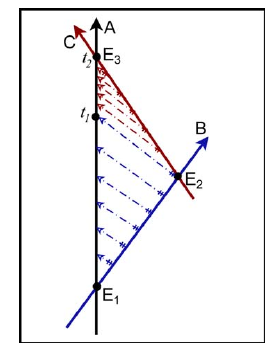
\includegraphics[scale=1]{immagini/conferme_relspec/radargemelli.png}
   \caption{\label{radar_gemelli}Il metodo radar.}
\end{figure}

Rispondiamo alla domanda facedo uso del metodo radar spiegato sopra e illustrato 
in \ref{radar_gemelli}.

Per confrontare i tempi trascorsi usiamo il metodo dello scambio di segnali
luminosi (metodo che sta alla base della geometria di Minkowski). Suppo-
niamo che, mentre si allontana, $B$ invii $n$ segnali luminosi con periodo $T$
(ad esempio, $n = 6$ e $T = 10 \min$, per fissare le idee). L'ultimo segnale ar-
riva ad $A$ al suo tempo $t_1$ . Supponiamo poi che $C$ faccia la stessa cosa nel
suo avvicinarsi ad $A$: anch'esso invierà $n$ segnali con periodo $T$ , l'ultimo dei
quali è scambiato quando $C$ incrocia $A$, al tempo $t_2$ nel giudizio di $A$ (con
riferimento ancora alla figura \ref{radar_gemelli}).
Il tempo totale trascorso per il gemello $B + C$ è la somma dei periodi di
emissione dei segnali luminosi. Il tempo totale trascorso per $A$ è invece la
somma dei periodi di ricezione. Scindiamo le due diverse fasi.
Durante l'allontanamento di $B$ si ha che
\begin{equation}
T_{ric} = k \cdot T_{emiss} = kT 
\end{equation}

e dunque
\begin{equation}
 t_1 = nT_{ric} = kn \cdot T_{emiss} = knT = kT_B
\end{equation}
ove $T_B$ è la durata del tempo di viaggio di $B$.

Durante l'avvicinamento di $C$ si ha che
\begin{equation}
T_{ric} = \frac{1}{k} T_{emiss}
\end{equation}

e dunque
\begin{equation}
t_2 - t_1 = n T_{ric} = \frac{n}{k} T_{emiss} = = \frac{n}{k} T_{C}  
\end{equation}

ove $T_C$ è la durata del tempo di viaggio di $C$.

Dato che, per simmetria, i due tempi di viaggio di $B$ e $C$ devono essere
uguali, $T_B$ = $T_C$ , ricaviamo che:

\begin{equation}
\begin{split}
t_2 &= t_1 + (t_2 - t_1 ) = kT_B + k^{-1} T_C = (k + k ^{- 1})T_B = \frac{1}{2}(k + k^{- 1})2 T_B = \\
&= \frac{1}{2} (k + k^{-1})(T_B + T_C ) = \gamma(v) \cdot (T_B + T_C )
\end{split}
\end{equation}

Dunque il tempo totale trascorso per $A$ è $\gamma(v)$ volte la somma dei tempi
trascorsi per $B$ e per $C$, cioè $\gamma(v)$ volte il tempo totale trascorso per il
gemello $B + C$. Evidentemente, i due tempi coincidono solo se $v = 0$; ne
concludiamo che il gemello $A$ (che non si è allontanato) è invecchiato di più
rispetto all'altro gemello $B + C$.

Nasce però un'obiezione sensata: questa conclusione sembra violare il Principio di Relatività!
Il moto è infatti relativo, quindi non si può dire se sia
il gemello $B + C$ ad allontanarsi da $A$ o se sia invece $A$ che si allontana a
sinistra da $B + C$ e poi si riavvicina. Se le due situazioni sono indistinguibili,
allora gli effetti devono essere uguali, e perciò $B + C$ deve invecchiare più di
$A$! C'è una contraddizione logica nella geometria di Minkowski? Quindi la
geometria di Minkowski non sta in piedi? Dove sta l'inghippo?
Sia $A$ sia $B + C$ vedono accadere $E_1$ ed $E_3$ nello stesso luogo, ma tra
questi due gemelli c'è una differenza fondamentale: uno dei due non è un
vero e proprio osservatore inerziale, o meglio, c'è un istante in cui egli cessa
di essere un osservatore inerziale. Il punto chiave è l'inversione del moto:
nel punto di inversione del moto, il gemello $B + C$ smette infatti per un
attimo di essere inerziale: i suoi pendoli e i suoi giroscopi impazziranno,
onde poi riprendere il normale comportamento nella fase di ritorno. Questa
differenza che pare microscopica, è in realtà assai significativa: $A$ è sempre
un osservatore inerziale, $B + C$, per un pur breve istante, non lo è.

La risposta è quindi che la situazione non è simmetrica. Per rimanere nel
campo degli osservatori inerziali dobbiamo confrontare $A$ con due osservatori
($B$ e $C$), situazione palesemente asimmetrica! 
Stiamo quindi confrontando un osservatore inerziale con un osservatore
non inerziale, e perciò non possiamo invocare il Principio di Relatività.

\begin{figure}[htbp]
   \centering
   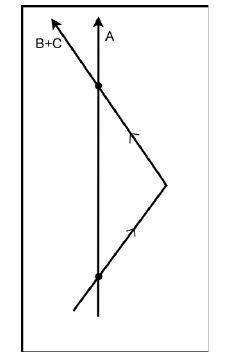
\includegraphics[scale=1]{immagini/conferme_relspec/dis_triang_mink.png}
   \caption{\label{dis_triang_mink}La disuguaglianza triangolare nello spaziotempo di Minkowski è invertita.}
\end{figure}

Nella geometria di Minkowski, questa asimmetria si manifesta nel fatto
che confrontiamo un segmento del genere tempo (quello di $A$) con una spezzata
del genere tempo (quella di $B+C$) - v. fig. \ref{dis_triang_mink}. Abbiamo quindi trovato
che nella geometria di Minkowski, per triangoli del genere tempo, vale la disuguaglianza
triangolare invertita: un lato è maggiore o uguale della somma
degli altri due lati. 

Questo è il significato geometrico del paradosso dei gemelli. 
Da questo punto di vista, tale paradosso non è altro che lo studio
della geometria di un triangolo del genere tempo in $M$ e la scoperta della
disuguaglianza triangolare invertita.


\begin{figure}[htbp]
   \centering
   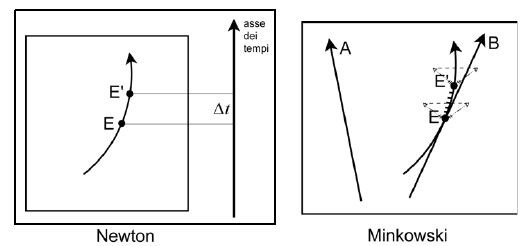
\includegraphics[scale=1]{immagini/conferme_relspec/tempi.png}
   \caption{\label{tempi}Differenza nella concezione degli intervalli di tempo tra lo 
schema classico e lo spaziotempo di Minkowski. Nello spaziotempo newtoniano le durate hanno carattere assoluto. 
Nello schema minkowskiano, le durate sono lunghezze d'arco, dipendono dal percorso.}
\end{figure}

Il paradosso dei gemelli ci fa capire la natura del tempo relativistico: il tempo è una lunghezza d'arco,
ovvero le durate dipendo dal percorso, esattamente come lo spazio percorso.

\subsection{Esperimento di Hafele-Keating}

Nel 1972 si è avuta la prima verifica sperimentale del paradosso dei gemelli
fuori dai laboratori, con l'esperimento di Hafele-Keating. Essi hanno preso
tre orologi atomici identici, ne hanno lasciato uno a terra (a Baltimora) e
hanno posto gli altri due in volo su aerei di linea, lanciati in versi opposti a
fare il giro equatoriale della terra\footnote{L'utilizzo di due aerei in luogo di uno solo è
per ovviare ad alcuni effetti gravitazionali inevitabilmente presenti e dovuti alla rotazione terrestre.}.

Ciò costringe i tre orologi a percorrere tre linee di universo diverse nello spaziotempo, 
ma avendo due eventi coincidenti: l'evento $E_0$ di partenza di due aerei e l'evento $E_1$ di ritrovo dei tre orologi
dopo il giro del mondo degli aerei.

\begin{figure}[htbp]
   \centering
   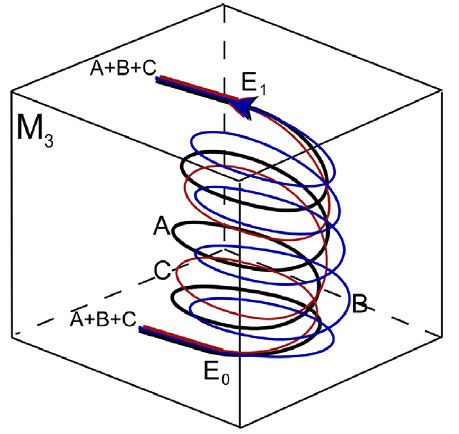
\includegraphics[scale=1]{immagini/conferme_relspec/hafele_keating.png}
   \caption{\label{hafele_keating} Esperimento di Hafele-Keating. $A$ (linea nera) è l'orologio
fermo a Baltimora; $B$ è l'orologio collocato sull'aereo in viaggio equatoriale
nello senso di rotazione terrestre. $C$ è l'orologio collocato sull'aereo in viaggio
in verso contrario rispetto al senso di rotazione terrestre. Tutte le linee di
universo sono, in prima approssimazione eliche cilindriche. Prima di $E_0$ (par-
tenza) e dopo $E_1$ (ritrovo) esse coincidono completamente. Tra i due eventi, le
eliche degli osservatori hanno passi diversi. La differenza dei percorsi fatti da
$A$, $B$ e $C$ tra $E_0$ ed $E_1$ si ripercuote in una differenza di cammino percorso, ma
anche di tempo trascorso - essendo il tempo in tutto e per tutto una lunghezza
d'arco, esso dipende infatti dal cammino di integrazione.}
\end{figure}

La figura \ref{hafele_keating} riporta le linee di universo di tali orologi in uno spazio
bidimensionale (supponiamo che lo spazio sia la sezione terrestre, tagliata
equatorialmente con il piano su cui circolano ambedue gli aerei in moto). Sia
$A$ l'orologio dermo a Baltimora, siano $B$ e $C$ gli orologi in viaggio sugli aerei.
$A$ non è inerziale, si muove con la rotazione terrestre. Per quanto riguarda
gli orologi $B$ e $C$, anche le loro linee di universo saranno eliche cilindriche,
ma aventi passi diversi, strutturate in modo diverso. Ciò che accomuna le tre
linee di universo è il fatto che esse differiscono solamente nei tratti compresi
tra gli eventi $E_0$ ed $E_1$ : prima della partenza e dopo l'arrivo, infatti, i tre
orologi sono tutti situati a Baltimora, nel medesimo luogo, ove ritornano alla
fine del viaggio.
Nella figura \ref{hafele_grafico} si può vedere come l'effetto risulti evidente dai
dati sperimentali.
Il fatto significativo è che nel tratto in cui le tre linee si distinguono,
i tre orologi battono diversamente: all'arrivo a Baltimora, gli orologi $B$ e
$C$ in viaggio hanno battuto più lentamente, e segnano di conseguenza un
tempo leggermente inferiore all'orologio $A$, sempre solidale con la terra -
una differenza leggera, ma rilevabile e rilevata dall'esperimento. Se al posto
dell'orologio e degli aerei, avessimo tre macchine e tre contachilometri non ci
stupiremmo affatto di questo risultato: ci sembrerebbe assai naturale che le
tre auto, partite da $E_0$ , giunte a $E_1$ tramite percorsi diversi, abbiano percorso
un diverso numero di chilometri. Questo accade in maniera del tutto analoga
anche per i tempi, poichè il tempo nello spaziotempo di Minkowski è una
lunghezza d'arco, e come tale va trattata. Integrando su cammini diversi,
otteniamo risultati diversi.
\begin{figure}[htbp]
   \centering
   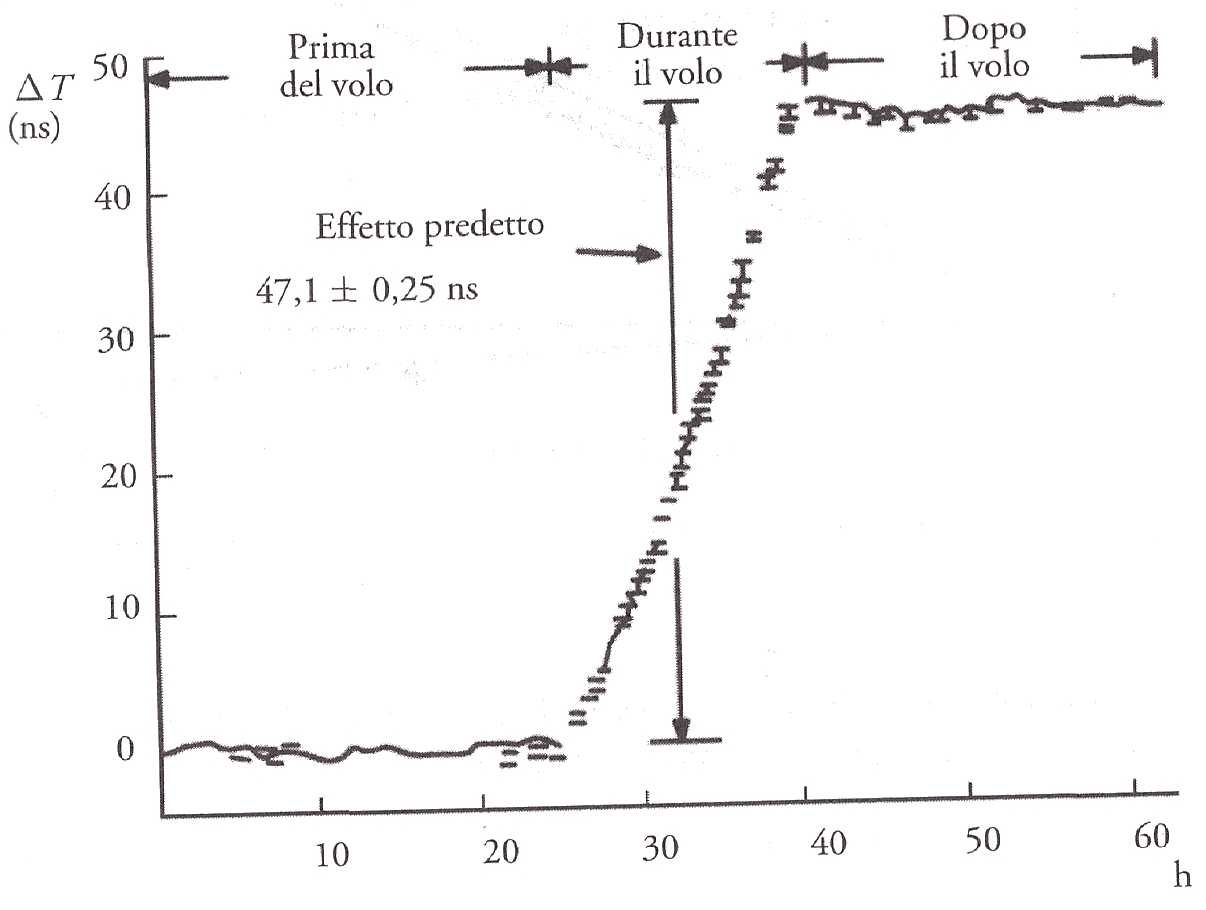
\includegraphics[scale=0.2]{immagini/conferme_relspec/hafele_grafico}
   \caption{\label{hafele_grafico} Esperimento di Hafele-Keating: in ascisse è riportato il tempo
durante il quale è stata controllata la marcia degli orologi, mentre in ordinate è riportata la differenza
fra i tempi da essi marcati.}
\end{figure}
\chapter{Relatività generale}

Torniamo per un attimo ad assumere un punto di vista cronologico. Una
volta messa a punto la geometria dello spazio di Minkowski (cioè della relatività 
ristretta), si aprivano di fronte a Einstein due problemi a prima vista
scorrelati.

\begin{enumerate}
 \item[i)] In primo luogo, tutta la teoria relativistica svolta sino ad ora ha utilizzato 
il concetto di osservatore inerziale ed ha avuto come scopo la
scrittura delle equazioni della fisica in una forma indipendente dalla
scelta dell'osservatore inerziale, al fine di mostrare la compatibilità di
tali equazioni con il Principio di Relatività. 
Il problema di Einstein nel 1906 è dunque quello di estendere la teoria precedente, così da
conglobare in essa anche osservatori non inerziali, con il proposito di
scrivere le equazioni della fisica in una forma che sia invariante nel passaggio 
da un osservatore a un altro. Lo scopo è quindi il superamento del concetto di osservatore inerziale e della cosiddetta 
formulazione covariante\footnote{Cioè formulazione indipendente dal sistema di riferimento inerziale scelto. Nella sua
forma estesa, la formulazione indipendente dall'osservatore (qualsiasi) scelto verrà detta ``formulazione covariante generale''}
delle equazioni della fisica.
È dunque in questo senso che questa parte della teoria è stata denominata da 
Einstein Relatività Generale (dal momento che considera la classe generale 
degli osservatori, pensati sempre come sistemi di coordinate sullo spaziotempo), per contrasto con la parte della teoria basata
sull'uso dei soli osservatori inerziali (detta Relatività Ristretta)\footnote{Va 
sfatato un deleterio luogo comune: si legge e si sente dire spesso che la Relatività
Ristretta si applica solo ai sistemi di riferimento inerziali, cioè al caso di moti non accelerati. 
Non c'è nulla di più falso: la Relatività Ristretta va bene per qualsiasi tipo di moto, nell'ipotesi che 
lo spaziotempo sia piatto, ossia nell'ipotesi di assenza di gravità. Addirittura, 
la Relatività Ristretta nasce dalle simmetrie dell'elettromagnetismo, e dunque non
ha alcun problema a contemplare (ad esempio) elettroni accelerati.}.

 \item[ii)] D'altro canto, il proposito della Relatività Ristretta di scrivere le equazioni 
della fisica in forma invariante rispetto al gruppo di Lorentz (cioè
rispetto al cambio di osservatore inerziale) doveva ancora essere completato. 
Dopo aver realizzato questo scopo per la meccanica della particella, per la meccanica dei fluidi 
e per 
l'elettromagnetismo\footnote{Ricordiamo che, se per rendere compatibili le equazioni della meccanica con il Principio
di Relatività abbiamo dovuto modificare le equazioni di Newton, le equazioni dell'elettromagnetismo erano 
già compatibili con tale principio, e quindi invarianti per trasformazioni di Lorentz.},
rimaneva da trattare la gravitazione. E ovvio che la gravitazione newtoniana, 
basata sul concetto di simultaneità assoluta e di azione a distanza istantanea, non è compatibile con i principi 
della Relatività Ristretta\footnote{Difatti, l'asserto newtoniano secondo cui due masse a distanza $r$ esercitano una forza
diretta lungo la congiungente in verso centripeto e proporzionale a $r^{-2}$ , presuppone che
spostando una delle due masse l'informazione arrivi all'altra massa istantaneamente, e
dunque che la forza vari istantaneamente (concetto di azione a distanza istantanea). Inol-
tre per avere la distanza tra le due particelle dobbiamo compiere le misurazioni in uno
stesso istante, il che implica che deve esserci simultaneità assoluta.};
si tratta quindi di riaffrontare il problema.
\end{enumerate}

La prima idea è che bisogna procedere con le equazioni di Newton del 
campo gravitazionale così come abbiamo fatto per le equazioni newtoniane 
della dinamica, cioè modificandole (senza stravolgerle) per renderle compatibili 
con la geometria dello spaziotempo di Minkowski, di cui lo spaziotempo newtoniano 
non è altro che un'approssimazione locale. Si può qualificare questo secondo problema 
come il problema di conglobare la teoria della gravitazione nello
spaziotempo di Minkowski.

Tuttavia si scopre che la gravitazione comporta la modifica della struttura
dello spaziotempo di Minkowski. Il fulcro è dunque che la teoria della gravitazione 
si identifica con la geometria dello spaziotempo, il quale acquista un carattere dinamico.

Dal punto di vista della prospettiva storica attuale, i due problemi, che
per Einstein avevano uguale importanza, svolgono un ruolo completamente
diverso. I problemi della Relatività Generale e del principio di covarianza
generale\footnote{Cioè il principio secondo cui le leggi fisiche devono essere le stesse per ogni sistema
di riferimento. Si noti che da tale principio consegue quasi immediatamente che lo strumento 
matematico per la descrizione della Relatività Generale non può che essere il calcolo
tensoriale.} - punto (i) - hanno poi assunto un carattere via via più secondario.
Nella prospettiva moderna, la teoria della Relatività Generale è definita
come la teoria della gravitazione einsteiniana, identificata con lo studio della
geometria dello spaziotempo - punto (ii).

\section{Forze apparenti}

Passando da un osservatore inerziale ad un osservatore non inerziale
bisogna introdurre le cosiddette forze apparenti. 

Mettiamoci infatti nell'ottica dello schema newtoniano (l'unico che al riguardo per ora conosciamo); 
il primo carattere delle forze apparenti è di essere strettamente proporzionali alla massa inerziale della particella 
su cui si esercitano\footnote{
Ad esempio la forza di Coriolis è data da:
\[F_{Coriolis} = -2m \omega  \wedge v r\]}.

Il secondo carattere delle forze apparenti è (appunto!) di essere apparenti:
il che, per definizione, significa che esse possono essere rigorosamente e globalmente 
annullate semplicemente cambiando osservatore, cioè passando dall'osservatore di cui si sta studiando 
il moto a un cert'altro osservatore. Sappiamo che quest'altro osservatore sarà accelerato rispetto al primo.

Questa caratteristica è detta proprietà di annullamento globale delle forze apparenti: basta cambiare osservatore, 
e rispetto a questo nuovo osservatore immediatamente tutte le forze apparenti scompaiono.

\subsection{Caratteri della forza gravitazionale}
La prima proprietà delle forze apparenti (proporzionalità alla massa iner\-ziale $m_i$) è
 rigorosamente condivisa dalla forza di gravitazione: è noto infatti che tutte le particelle, 
in un campo gravitazionale uniforme e stazionario, ca\-dono con la stessa accelerazione $g$, 
detta accelerazione di gravità. 

Quindi, per la legge di Newton
\begin{equation}
F_{grav} = m_{i} · g
\end{equation}
dove $m_i$ è la massa inerziale. In questo modo si ottiene che:
\begin{equation}\label{massa_inerz}
m_i · a = F_{grav} = m_i · g
\end{equation}
da cui
\begin{equation}
a = g
\end{equation}
e quindi tutte le particelle cadono con uguale accelerazione.
Per sottolineare questo fatto si usa introdurre una ``carica gravitazionale''
$m_g$, detta massa gravitazionale, e scrivere che:
\begin{equation}
F_{grav} = m_g \cdot g,
\end{equation}
in analogia con la formula della forza elettrica:
\begin{equation}
F_{elettr} = q \cdot E
\end{equation}

Possiamo quindi riscrivere l'equazione \ref{massa_inerz} come
\begin{equation}
m_i \cdot a = m_g \cdot g
\end{equation}
e la proprietà scoperta da Galileo dell'universalità dell'accelerazione di gra\-
vità si esprime quindi dicendo che:
\begin{equation}\label{principio_equivalenza_debole}
m_i = m_g 
\end{equation}
La \ref{principio_equivalenza_debole} è detta principio di equivalenza debole: lo assumeremo
come un postulato\footnote{Il più famoso esperimento che lo avvalora è l’esperimento di Eotvos, di bilanciamento
tra forze gravitazionali e forze apparenti (per approfondimenti: \url{http://it.wikipedia.org/wiki/Esperienza_di_Eotvos}.};
esso ci garantisce che (per qualche strana ragione che può apparire quasi ``magica'') massa gravitazionale e massa inerziale
coincidono sempre.
Anche la seconda proprietà delle forze apparenti (la proprietà di an\-nullamento, che giustifica il loro nome di ``forze apparenti'')
è condivisa dalle forze gravitazionali, ma con un'importante differenza: essa vale ora solo localmente.

\section{Osservatori in caduta libera}
Per comprendere questo fatto, consideriamo anzitutto il caso speciale di
un campo gravitazionale uniforme (costante) nello spazio e stazionario nel
tempo; quindi $\vec{g}$ è un vettore costante nello spaziotempo rispetto ad un opportuno 
osservatore inerziale. Proprio per il principio di equivalenza debole,
possiamo annullare il campo gravitazionale in ogni punto dello spazio semplicemente 
passando ad un osservatore in caduta libera, cioè un osservatore
non inerziale, che si muove rispetto all'osservatore inerziale precedente con
un'accelerazione $a = g$. 
Rispetto a tale osservatore, secondo le leggi della
dinamica di Newton, una certa particella di prova si muove sotto l'azione
combinata della gravitazione (dovuta al fatto che essa è in un campo gravitazionale) 
e della forza apparente di gravitazione (dovuta al fatto che stiamo
considerando un osservatore non inerziale). Dunque l'equazione di moto è
$m_i a_{rel} = F_{grav} + F_{app} = m_g g + mi (-aapp ) = mg g - mi aapp = 0$,
dove $arel$ è l'accelerazione totale della particella relativa all'osservatore in caduta 
libera, $F_grav$ è la forza gravitazionale agente sulla particella e $F_app$ è la
forza apparente (detta anche forza di trascinamento) che agisce sulla parti-
cella in virtù del fatto che siamo in un riferimento non inerziale. Abbiamo
usato nell'ultimo passaggio il principio di equivalenza debole ($m_g = m_i$) e
il fatto che, per l'osservatore in caduta libera, l'accelerazione apparente di
trascinamento eguaglia in modulo esattamente l'accelerazione gravitazionale,
ed è di verso opposto a questa. Perciò nel campo gravitazionale costante e
stazionario la particella si muove, rispetto all'osservatore in caduta libera,
come se fosse libera, come se non fosse soggetta ad alcuna forza.
Poiché ogni campo gravitazionale può essere localmente\footnote{
Qui ``localmente'' deve essere inteso in senso spaziotemporale, 
cioè per ``piccole'' regioni di spazio, così piccole da poter considerare $\vec{g}$ 
uniforme in tale regione) e per ``brevi'' intervalli di tempo,
così brevi che la particella di prova non esca, in questo intervallo di
tempo, dalla regione in cui $g$ può essere considerato uniforme.} considerato costante, 
ne segue che la proprietà di annullamento, globale per ogni campo
uniforme e stazionario, vale localmente per ogni campo gravitazionale\footnote{È 
questa la situazione di ``moto in assenza di peso'' che si verifica, ad esempio, in ogni
navicella spaziale orbitante attorno alla terra: in assenza di spinta dei motori, essa si trova
infatti in caduta libera rispetto alla terra (``cade'' infatti sulla terra con un'accelerazione
centripeta g), e dunque la gravità terrestre è localmente annullata.}.

\subsection{Origine degli osservatori inerziali}
L'aver collegato il concetto di osservatore (localmente) inerziale alla geometria 
dello spaziotempo, e quindi in senso fisico alla geometria dell'universo,
ha anche un aspetto soddisfacente da un punto di vista fisico. Un problema
generale che ha assillato i fisici\footnote{In effetti, questo è un punto critico assai problematico 
per la fisica in generale.},
da Newton in avanti, era di spiegare da che cosa fossero determinati gli osservatori 
inerziali, perché cioè un certo osservatore fosse inerziale, mentre un altro non lo fosse. 
Newton rispondeva a
questa domanda con l'assioma dello spazio assoluto: gli osservatori inerziali
sono dunque quelli in quiete rispetto allo spazio. Questa giustificazione non
può più funzionare per Einstein.

La verifica sperimentale che nel nostro sistema solare gli osservatori iner-
ziali fossero in qualche modo legati alla materia distante (al ``cielo delle stelle
fisse'') aveva portato Mach a sviluppare l'idea che gli osservatori inerziali 
dovessero essere definiti dalla distribuzione di materia nell'universo\footnote{
In sostanza, Mach ritiene che se ci fosse un solo corpo nello spazio vuoto non avrebbe
nemmeno senso la nozione di osservatore inerziale.}. 

Gli osservatori inerziali sarebbero quindi corpi in una particolare relazione con 
la materia distante (principio o punto di vista di Mach).

Einstein riprende il punto di vista di Mach e lo realizza compiutamente:
comprendendo che la materia fissa la geometria dello spaziotempo e sapendo
che la geometria fissa gli osservatori localmente inerziali, egli realizza con-
cretamente il legame tra materia distante\footnote{
Perché ``distante''? Perché per fissare la curvatura dello spaziotempo in un punto non
è sufficiente la materia nel punto: servono le derivate prime dei simboli di Christoffel, cioè
le derivate seconde della metrica, e dunque entra in gioco la materia distante.} 
e osservatori inerziali. Quindi, l'idea degli osservatori in caduta libera realizza il principio di Mach.

\subsection{Il principio di equivalenza forte}
Una volta arrivati a questo concetto è naturale assimilare gli osservatori in
caduta libera agli osservatori inerziali dello spaziotempo di Minkowski, accettando 
che nei riferimenti degli osservatori in caduta libera i fenomeni fisici
avvengano localmente tutti con le stesse modalità (a parità di condizioni
ambientali) e che le leggi della fisica assumano in tali riferimenti la forma
minkowskiana. Questa affermazione prende il nome di principio di equivalenza forte: 
esso postula la completa equivalenza (locale) degli osservatori
in caduta libera con gli osservatori inerziali di minkowskiana memoria\footnote{
In altre parole, postula che localmente gravità e accelerazione siano indistinguibili.
Naturalmente questo vale solo localmente: se lasciamo cadere due palline in un razzo in accelerazione,
tali palline seguiranno sempre traiettorie parallele, mentre se lasciamo cadere
le stesse palline da posizioni molto diverse della superficie terrestre, entrambe si indirizzeranno 
verso il centro della terra (con evidente rottura della simmetria tra accelerazioni
apparenti e gravità).}.

Nello stesso ordine di idee è naturale assimilare le particelle in caduta
libera (cioè non soggette a forze di natura diversa dalla forza gravitazionale)
alle particelle libere tout-court di Newton, e quindi postulare che le linee di
universo di tali particelle siano geodetiche del genere tempo nello spaziotempo
(principio della geodetica). Tornando all'analogia con il trampolino di
figura 10.3, un oggetto di prova (ad esempio: una pallina di ping-pong)
posizionato sul trampolino incurvato, accelererà verso la sfera centrale in
un modo governato dalla curvatura stessa del trampolino. Il principio della
geodetica ci dice come la curvatura dello spaziotempo (cioè del trampolino)
governa il moto della materia: i corpi in caduta libera (come la pallina da
ping-pong) seguono geodetiche nello spaziotempo. Ad esempio, inviando la
pallina con la giusta velocità e direzione, essa inizierà a orbitare intorno alla
palla di marmo centrale (come la luna orbita intorno alla terra).
Concettualmente, abbiamo sostituito all'idea di forza gravitazionale la
geometria: la traiettoria della pallina da ping-pong non è più dovuta alla
gravità, piuttosto diciamo che è dovuta alla curvatura dello spaziotempo e
al principio che vuole la traiettoria della pallina essere una geodetica in tale
spaziotempo. In generale stiamo considerando fenomeni che classicamente
erano legati all'azione della gravità (come la caduta dei gravi o il moto di
una navicella orbitante) come fenomeni di caduta libera, che localmente sono
a tutti gli effetti inerziali\footnote{
Così ad esempio, quando percepiamo, stando sulla superficie terrestre, una ``forza di
gravità'', essa è sostanzialmente un risultato del fatto che, non essendo noi osservatori
in caduta libera, siamo continuamente sottoposti a un'accelerazione fisica causata dalla
resistenza meccanica della superficie terrestre.}.

La presenza di un campo gravitazionale non uniforme, che quindi non può
essere annullato globalmente e che implica la curvatura dello spaziotempo, si
manifesta nel fenomeno di deviazione geodetica che studieremo tra poco.






\chapter{Conferme sperimentali della relatività speciale}
\minitoc

\section{Paradossi}
Riassumiamo brevemente alcuni degli effetti paradossali predetti dalla Rela-
tività Generale che abbiamo trovato nelle sezioni precedenti, insieme ad altri
che non abbiamo analizzato e cui accenniamo solo brevemente.

\begin{itemize}
 \item Deviazione geodetica: a causa della curvatura dello spaziotempo due
geodetiche localmente vicine possono divergere; questo si traduce ad
esempio nel cambio di orientazione nel tempo di un giroscopio orbitante.
 \item Precessione dei perieli: i semiassi delle orbite planetarie ruotano
(``precedono'') nel tempo più di quanto la teoria della gravità newtoniana 
avesse predetto. La conferma sperimentale più importante è stata la precessione 
del perielio di Mercurio, la cui marcata orbita a ``rosetta'' è 
in linea con i calcoli teorici della Relatività Generale.
 \item Buchi neri: come previsto dalla teoria di Schwarzschild, i buchi neri
sono corpi aventi raggio di Schwarzschild maggiore del proprio raggio,
in cui le informazioni entranti non potranno mai più essere recuperate\footnote{
Più recentemente sono nate molte altre variegate teorie al riguardo.}.
 \item Deviazione dei raggi luminosi: a causa della gravità, anche le onde
luminose e i segnali radar incurvano la loro traiettoria. In particolare,
se lo spazio è incurvato dal campo gravitazionale solare, un raggio di
luce che passa nelle vicinanze del sole non compierà un cammino rettilineo: 
dunque le stelle la cui luce ci giunge passando vicino al sole
ci appariranno in una posizione leggermente deviata dalla loro posizione 
effettiva. Di questo fatto di cui si è avuta conferma sperimentale
osservando pulsar passare dietro al sole durante le eclissi di sole.
 \item Dilatazione gravitazionale dei tempi: il tempo scorre più lentamente 
ove il campo è piè intenso.
Per convincerci di ciò, consideriamo la figura XXX: A è un osservatore 
posto al centro di un disco rotante, B è un osservatore
posto sul bordo del disco rotante, C è un osservatore inerziale posto
a terra, al di fuori del disco rotante. Dato che A e C sono in quiete
relativa, vedranno scorrere il tempo nello stesso modo. Dato inoltre che
B è in moto, nel giudizio di C, allora C vedrà l'orologio di B battere
più lentamente, e dunque anche A dovrà vedere l'orologio di B battere
più lentamente.
D'altro canto, anche A e C sono in quiete relativa, poiché sono entrambi
sulla piattaforma rotante. E se per C il fatto che l'orologio di B batta
più lentamente si pu` spiegare quindi con il fatto che B è in moto
relativo rispetto a C, questo non regge più per A, poiché non v'è alcun
moto relativo tra A e B sulla disco, c'é solo un campo di accelerazioni
centripete verso il centro del disco. Ne discende che, nel giudizio di
A, il tempo scorre più lentamente verso il bordo, e ricordando che
l'accelerazione centripeta è data da $2 \omega r$, possiamo anche generalizzare
dicendo che gli orologi battono più lentamente laddove il campo è più
forte.
 \item Lunghezza delle circonferenze: dall'esperimento mentale appena
esposto si deduce anche un altro fatto curioso. Se posizioniamo (a
riposo) dei metri lungo la circonferenza del disco e lungo il suo diametro,
troveremo che naturalmente il rapporto tra il numero di metri usati sarà
$\pi$. Se immaginiamo ora che la piattaforma si metta a ruotare, mentre
i metri posti lungo il diametro (ortogonali al moto) non cambieranno
lunghezza, i metri posti lungo la circonferenza (longitudinali al moto) si
accorceranno, e dunque avremo bisogno di più metri per coprire tutta
la circonferenza. Esibendo un rapporto tra circonferenza e diametro
che non è più il valore costante $\pi$, questo esperimento curioso mostra
anche che la geometria della Relatività Generale non può più essere la
geometria euclidea o semieuclidea.
 \item Red-shift gravitazionale: fenomeno direttamente derivante dalla dilatazione 
gravitazionale dei tempi. A causa della deformazione spazio-temporale 
prodotta dal campo gravitazionale solare, ad esempio, vediamo 
le righe degli spettri degli atomi solari eccitati a una frequenza
minore di quella che vedremmo per atomi eccitati sulla terra.
 \item Espansione dell'universo: le prime soluzioni cosmologiche alle equa-
zioni di campo di Einstein prevedevano un universo in espansione, fatto
confermato dagli esperimenti di Edwin Hubble nel 1921.
\end{itemize}

\section{Un'applicazione: il GPS}

Il Selective Availability è un sistema di generazione di errori voluto espressamente dal Dipartimento della Difesa 
statunitense per consentire il Global Positioning System (GPS) per usi civili.

Nel 1991, infatti, venne reso disponibile per usi civili il sistema Standard Positioning System (SPS), 
che introduceva volutamente degli errori mediante il Selective Availability in modo da rendere inaccurati i valori.

Dal 2000 si è rinunciato alla Selective Availability e l'SPS è divenuto accurato quasi quanto il 
Precision Positioning System (PPS), usato per scopi militari.

Gli orologi satellitari sono affetti dalle conseguenze della teoria della relatività. 
Infatti, a causa degli effetti combinati della velocità relativa, che rallenta il tempo sul satellite di circa 
7 microsecondi al giorno, e della minore curvatura dello spaziotempo a livello dell'orbita del satellite, 
che lo accelera di 45 microsecondi, il tempo sul satellite scorre ad un ritmo leggermente più veloce che a terra, 
causando un anticipo di circa 38 microsecondi al giorno, e rendendo necessaria una correzione automatica da parte 
dell'elettronica di bordo. 

Questa osservazione fornisce un'ulteriore prova dell'esattezza della teoria einsteniana 
in un'applicazione del mondo reale. L'effetto relativistico rilevato è, infatti, esattamente corrispondente a quello 
calcolabile teoricamente, almeno nei limiti di accuratezza forniti dagli strumenti di misura 
attualmente disponibili. Possono, inoltre, esistere altri tipi di errori del GPS che sono appunto 
di tipo atmosferico e di tipo elettronico.

È di fondamentale importanza ribadire che quello che permette al GPS la precisione cui 
si arriva (incertezze di pochi metri), sono proprio le correzioni di relatività generale; 
quelle della relatività ristretta, che ignorerebbero l'effetto sugli orologi dei satelliti, 
darebbero incertezze dell'ordine del chilometro che renderebbero il sistema del tutto inutile.

\url{http://www.astronomy.ohio-state.edu/~pogge/Ast162/Unit5/gps.html}
\url{http://it.wikipedia.org/wiki/Selective_Availability}

\section{Guardando avanti}

In un certo senso, questo è solo l'inizio della Relatività Generale, il cui ulteriore 
studio si intreccia poi naturalmente con la cosmologia, per cui la
Relatività Generale costituisce un ottimo modello geometrico gravitazionale,
un modello che ha superato indenne tutti i test sperimentali seri cui è stato
sottoposto negli ultimi decenni.

D'altro canto, il problema più serio è che la Relatività Generale è in aperto
conflitto con la meccanica quantistica; le predizioni relativistiche che sembrano 
valere ``nel grande'' sicuramente non valgono ``in piccolo'': la necessità
dei fisici è quindi ora quella di unificare questi due mondi così diversi 
(Relatività e Meccanica Quantistica), riuscendo a costruire una teoria coerente e
consistente, che possa inglobarle con successo.

%**************************INIZIO APPENDICI************************************
\appendix
\chapter[Credits]{Credits}

Questo mini-corso è stato costruito \sout{copiando spudoratamente} prendendo ispirazione da due fonti principali:
\begin{itemize}
 \item le dispense preparate da R. Turra a partire dalle lezioni di Fisica 1, 2, 3 seguite all'università di Milano-Bicocca.
 \item le ``Dodici lezioni sulla relatività'' del prof. F. Magri, scritte, integrate e organizzate da D. Ghisi
\end{itemize}

Ovviamente, ``ça va sans dire'', durante il lavoro di copia-incolla-taglia-cuci probabilmente ho introdotto numerosi errori e i cambiamenti di 
stile e di notazione tra le varie parti del testo dovrebbero essere oltremodo evidenti. Ovviamente mi prendo la responsabilità di tutto questo
e mi dispiace di avere senza dubbio rovinato la compattezza delle dispense di Fisica e 
l'eleganza delle lezioni di Relatività.

Vi prego infine di ricordare che queste dispense sono assolutamente una bozza preliminare, numerosi sono i punti da chiarire e da integrare
per rendere questo testo un vero ``Mini-corso sulla Relatività''.

Potete contattarmi scrivendo all'indirizzo:
\begin{center}
\framebox[1.1\width][c]{\textup{\textsf{\href{mailto://kikkocristian@gmail.com}{kikkocristian@gmail.com}}}}
\end{center}
\rmfamily\upshape

Infine, è doveroso ricordare che, a suo tempo, ho preparato degli esami studiando sulle dispense citate (in particolare ``Fisica 1 - mod I e II'' e ``Istituzioni 
di Fisica Matematica - mod. I'') incassando ottimi voti, colgo quindi l'occasione per ringraziare gli autori originali anche per questo. 

Sono riportati di seguito dei riferimenti a questi lavori.

\begin{itemize}
 \item Le dispense di R. Turra, riportavano il seguente disclaimer
\end{itemize}

\begin{quote}
\section*{\centering Disclaimer}
%\addstarredsection{Disclamer} % per minitoc
\addcontentsline{toc}{section}{\numberline{}Disclaimer}
Di questo documento puoi farne quello che vuoi, distribuirlo, fotocopiarlo, usare come carta per accendere il camino 
o per non sporcare per terra quando imbianchi i muri, a patto che l'autore originale 
e la sua email vengano riportati in modo significativo insieme a questo disclamer nella sua forma originale. 
Possono essere fatte modifiche solo allo scopo di migliorare il do\-cu\-men\-to. 
L'autore sarà felice di ricevere una copia di queste modifiche. 
In nessun caso questo documento, parti di esso o opere derivate potranno essere utilizzati come  fonte di lucro; 
l'unico eventuale ricavo ammesso è quello relativo alle spese di distribuzione, per esempio le spese di stampa. 
Questo documento non è la Bibbia, esso nasce per uso personale, ed è distribuito senza garanzia sui contenuti 
(se prendente un brutto voto studiando su questi appunti non prendetevela con me).

L'autore può essere contattato all'indirizzo:
\begin{center}
\framebox[1.1\width][c]{\textup{\textsf{\href{mailto://giurrero@gmail.com}{giurrero@gmail.com}}}}
\end{center}
\end{quote}
\rmfamily\upshape

La versione utilizzata per preparare il ``Mini-corso sulla Relatività'' è quella di aprile 2011 (Revision: $120$). 
I sorgenti sono disponibili all'indirizzo \href{http://code.google.com/p/fisica123}{http://code.google.com/p/fisica123}.

\begin{itemize}
 \item le dispense di D. Ghisi sono disponili all'indirizzo: 
\end{itemize}

\begin{center}
\framebox[1.1\width][c]{\textup{\textsf{\href{www.webalice.it/dghisi/scritti/relativita.pdf}{www.webalice.it/dghisi/scritti/relativita.pdf}}}}
\end{center}
\rmfamily\upshape

\section[Licenza]{Licenza}

Questo lavoro è disponibile secondo la licenza \textbf{Creative Commons - Attribuzione - Non commerciale - Condividi allo stesso modo}
(CC-BY-NC-SA) versione 3.0.

In sostanza è possibile riprodurre, distribuire, mettere a disposizione per lo scaricamento, 
comunicare al pubblico, esporre in pubblico, rappresentare, eseguire e recitare quest'opera
o modificarla a condizione di attribuire la paternità dell'opera riportando la seguente indicazione:
\begin{quote}

\textup{\textsf{Tratto da ``Un mini-corso sulla Relatività di Einstein''- di Cristian Consonni (da lavori precedenti di R. Turra e D. Ghisi)}}

\textup{\textsf{È possibile contattare l'autore orginale all'indirizzo kikkocristian@gmail.com.}}
\end{quote}

È inoltre necessario riportare il \textbf{Disclaimer} indicato da R. Turra e riportato sopra.
L'attribuzione di quest'opera in lavori derivati deve essere inserita in modo da non suggerire che gli autori originali 
avallino le opere derivate stesse o il modo in cui la loro opera è utilizzata.

Non è possibile quest'opera per fini commerciali, fatte salve le spese di distribuzione (ad es. rimborso spese di stampa).

Se si altera o trasforma quest'opera, o se la si usa per crearne un'altra, è possibile distribuire l'opera risultante solo 
con una licenza identica o equivalente a questa. 

Ulteriori informazioni ed il testo completo della licenza CC-BY-NC-SA sono disponibili alla 
pagina \url{http://creativecommons.org/licenses/by-nc-sa/3.0/deed.it}


%*****************************BIBLIOGRAFIA*************************************
\backmatter
\bibliography{TeX/fisica1/biblio}{}
\bibliographystyle{plain} %altri stili: prsty are abbrv, alpha, plain and unsrt

%********************************INDICE ANALITICO******************************

\ifpdf
\pdfbookmark{Indice analitico}{index}
\fi

\printindex

\typeout{}\typeout{}\typeout{}
\typeout{*******************************************************************************}
\typeout{RENDERING RIASSUNTI DI FISICA FINITO}
\typeout{*******************************************************************************}
\typeout{Magari ti e' andata bene}
\typeout{}\typeout{}\typeout{}

\end{document}
